% datastruct/datastruct.tex

\QuickQuizChapter{chp:Data Structures}{Data Structures}
%
\Epigraph{Bad programmers worry about the code. Good programmers worry
	  about data structures and their relationships.}
	 {\emph{Linus Torvalds}}

데이터로의 효율적인 접근은 중요해서, 알고리즘에 대한 논의는 관련된 데이터
구조의 시간 복잡도를 포함합니다~\cite{ThomasHCorman2001Algorithms}.
하지만, 병렬 프로그램에서는 시간 복잡도의 측정은 동시성에의 영향을 포함해야
합니다.
이런 영향은 Chapter~\ref{chp:Hardware and its Habits} 에서 보인 것처럼 지배적일
정도로 클 수 있는데, 이는 동시적인 데이터 구조의 설계는 순차적 시간 복잡도에
그러한 것만큼 동시성에도 신경을 써야 함을 의미합니다.
달리 말하자면, 훌륭한 병렬 프로그래머가 데이터 구조 관계에서 걱정해야할 중요한
부분 중 하나는 동시성에 관련된 부분입니다.
\iffalse

Efficient access to data is critically important, so that
discussions of algorithms include time complexity of the related
data structures~\cite{ThomasHCorman2001Algorithms}.
However, for parallel programs, measures of time complexity must also
include concurrency effects.
These effects can be overwhelmingly large, as shown in
Chapter~\ref{chp:Hardware and its Habits}, which means that
concurrent data structure designs must focus as much on
concurrency as they do on sequential time complexity.
In other words, an important part of the data-structure relationships
that good parallel programmers must worry about is that portion
related to concurrency.
\fi

Section~\ref{sec:datastruct:Motivating Application}
는 이 챕터에서 소개되는 데이터 구조들을 평가하는데 사용되며 모티베이션을 줄
어플리케이션을 선보입니다.

Chapter~\ref{cha:Partitioning and Synchronization Design} 에서 논의된 대로,
높은 확장성을 얻는 방법은 파티셔닝입니다.
이는 분할 가능한 데이터 구조를 위한 방법을 이야기 하게 되는데, 이 주제는
Section~\ref{sec:datastruct:Partitionable Data Structures} 에서 다룹니다.
Chapter~\ref{chp:Deferred Processing} 는 일부 동작들을 미뤄두는게 어떻게 성능과
확장성을 모두 크게 개선할 수 있는지 설명했습니다.
특히 Section~\ref{sec:defer:Read-Copy Update (RCU)} 에서는 성능과 확장성을
쫓음에 있어서 미뤄두기가 어떻게 대단한 효과를 보이는지를 보였는데, 이 주제는
Section~\ref{sec:datastruct:Read-Mostly Data Structures} 에서 다룹니다.
\iffalse

Section~\ref{sec:datastruct:Motivating Application}
presents a motivating application that will be used to evaluate
the data structures presented in this chapter.

As discussed in Chapter~\ref{cha:Partitioning and Synchronization Design},
an excellent way to achieve high scalability is partitioning.
This points the way to partitionable data structures, a topic taken up by
Section~\ref{sec:datastruct:Partitionable Data Structures}.
Chapter~\ref{chp:Deferred Processing} described how deferring some
actions can greatly improve both performance and scalability.
Section~\ref{sec:defer:Read-Copy Update (RCU)} in particular showed
how to tap the awesome power of procrastination in pursuit of
performance and scalability, a topic taken up by
Section~\ref{sec:datastruct:Read-Mostly Data Structures}.
\fi

모든 데이터 구조가 분할 가능하지는 않습니다.
Section~\ref{sec:datastruct:Non-Partitionable Data Structures} 는 다소
파티셔닝이 어려운 데이터 구조를 알아봅니다.
이 섹션은 이걸 어떻게 읽기가 대부분이고 파티셔닝 가능한 영역으로 쪼개서 빠르고
확장성 있는 구현을 가능하게 하는지 보입니다.
\iffalse

Not all data structures are partitionable.
Section~\ref{sec:datastruct:Non-Partitionable Data Structures}
looks at a mildly non-partitionable example data structure.
This section shows
how to split it into read-mostly and partitionable portions,
enabling a fast and scalable implementation.
\fi

이 챕터는 사용되어온 모든 동시적 데이터 구조의 자세한 부분들까지 이야기할 수는
없으므로
Section~\ref{sec:datastruct:Other Data Structures} 에서는 대부분의 유명하고
중요한 것들에 대한 간략한 조사 내용을 제공합니다.
최고의 성능과 확장성은 만들어진 내용에서의 세세한 최적화보다는 설계를
만들어내게 되긴 합니다만, 분명한 최고의 달성 가능한 성능과 확장성을 얻는데에
세세한 최적화가 중요한 위치를 차지하는건 분명합니다.
따라서 이 주제를
Section~\ref{sec:datastruct:Micro-Optimization} 에서 다루도록 합니다.

마지막으로, Section~\ref{sec:datastruct:Summary} 에서는 이 챕터의 요약을
제공합니다.
\iffalse

Because this chapter cannot delve into the details of every concurrent
data structure that has ever been used
Section~\ref{sec:datastruct:Other Data Structures}
provides a brief survey of the most common and important ones.
Although the best performance and scalability results design rather
than after-the-fact micro-optimization, it is nevertheless the case
that micro-optimization has an important place in achieving the
absolute best possible performance and scalability.
This topic is therefore taken up in
Section~\ref{sec:datastruct:Micro-Optimization}.

Finally, Section~\ref{sec:datastruct:Summary}
presents a summary of this chapter.
\fi

\section{Motivating Application}
\label{sec:datastruct:Motivating Application}

우리는 성능을 평가하는데에 Schr\"odinger 의 Zoo 어플리케이션을 사용하도록
하겠습니다~\cite{McKenney:2013:SDS:2483852.2483867}.
Schr\"odinger 는 많은 수의 동물을 수용하고 있는 동물원을 하나 가지고 있고, 그는
이 동물들을 in-memory 데이터베이스를 사용해 관리하려 할텐데, 동물원에 수용된
각각의 동물은 이 데이터베이스에 데이터 항목으로 표현됩니다.
각 동물은 키로 사용되는 유일한 이름을 가지고, 각 동물마다 관리되는 다양한
데이터를 갖습니다.

출산, 포획, 그리고 구매는 데이터 삽입이 되고, 사망, 방출, 그리고 판매는 삭제가
됩니다.
Schr\"odinger 의 동물원은 쥐와 곤충등을 포함해 많은 수의 단명하는 동물들을
수용하고 있으므로 이 데이터베이스는 높은 비율의 업데이트를 지원해야 합니다.
\iffalse

We will use the Schr\"odinger's Zoo application to evaluate
performance~\cite{McKenney:2013:SDS:2483852.2483867}.
Schr\"odinger has a zoo containing a large number of animals, and
he would like to track them using an in-memory database with
each animal in the zoo represented by a data item in this database.
Each animal has a unique name that is used as a key, with a variety
of data tracked for each animal.

Births, captures, and purchases result in insertions, while deaths,
releases, and sales result in deletions.
Because Schr\"odinger's zoo contains a large quantity of short-lived
animals, including mice and insects, the database must be able to
support a high update rate.
\fi

Schr\"odinger 의 동물들에 관심있는 사람들은 그것들에 대해 쿼리를 던질 수
있습니다만, Schr\"odinger 는 그의 고양이에의 굉장히 높은 비율의 쿼리가 존재함을
알렸고, 따라서 그는 그의 쥐들은 이 데이터베이스를 죽을 때에나 사용하게 될거라
생각합니다.
이말은 Schr\"odinger 의 어플리케이션은 하나의 데이터 항목으로의 높은 비율의
쿼리를 지원할 수 있어야 한다는 의미입니다.

다양한 데이터 구조들이 소개되는 중에도 이 어플리케이션을 마음속에 담아 두시기
바랍니다.
\iffalse

Those interested in Schr\"odinger's animals can query them, however,
Schr\"odinger has noted extremely high rates of queries for his cat,
so much so that he suspects that his mice might be using the database
to check up on their nemesis.
This means that Schr\"odinger's application must be able to support a
high rate of queries to a single data element.

Please keep this application in mind as various data structures are presented.
\fi

\section{Partitionable Data Structures}
\label{sec:datastruct:Partitionable Data Structures}

오늘날 사용되는 데이터 구조들은 굉장히 많아서, 그것들을 다루는 책도 여럿
있습니다.
이 작은 섹션은 하나의 데이터 구조인 해시 테이블에 집중해 봅니다.
이렇게 집중을 해보는 것은 어떻게 동시성이 데이터 구조와 상호작용하는지에 대한
깊은 이해를 가능하게 하고, 또한 실제 상황에서 굉장히 많이 사용되는 데이터
구조에 집중할 수 있게 합니다.
Section~\ref{sec:datastruct:Hash-Table Design} 에서는 이 디자인을 전체적으로
보고,
Section~\ref{sec:datastruct:Hash-Table Implementation} 에서는 그 구현을
제공합니다.
마지막으로,
Section~\ref{sec:datastruct:Hash-Table Performance} 에서는 그 결과로 나오는
성능과 확장성을 알아봅니다.
\iffalse

There are a huge number of data structures in use today, so much so
that there are multiple textbooks covering them.
This small section focuses
on a single data structure, namely the hash table.
This focused approach allows a much deeper investigation of how concurrency
interacts with data structures, and also focuses on a data structure
that is heavily used in practice.
Section~\ref{sec:datastruct:Hash-Table Design}
overviews of the design, and
Section~\ref{sec:datastruct:Hash-Table Implementation}
presents the implementation.
Finally,
Section~\ref{sec:datastruct:Hash-Table Performance}
discusses the resulting performance and scalability.
\fi

\subsection{Hash-Table Design}
\label{sec:datastruct:Hash-Table Design}

Chapter~\ref{cha:Partitioning and Synchronization Design}
에서는 괜찮은 성능과 확장성을 얻기 위해서는 파티셔닝을 적용해야 함을
알아보았고, 따라서 파티셔닝 적용 가능성은 데이터 구조를 선택할 때 첫번째로
고려할 기준이어야만 할 겁니다.
이 기준은 병렬성을 위해 많이 사용되는 해시 테이블에서 잘 만족됩니다.
해시 테이블은 개념적으로 간단하고, \emph{hash bucket} 들의 배열로 구성됩니다.
하나의 \emph{hash function} 은 주어진 원소의 \emph{key} 로부터 이 원소가
저장되게 될 hash bucket 으로의 매핑을 담당합니다.
따라서, 각각의 hash bucket 은 원소들의 링크드 리스트를 갖게되는데, 이는
\emph{hash chain} 이라 불립니다.
제대로 구성된다면, 이런 hash chain 들은 상당히 짧을 것이어서 해시 테이블이
주어진 키를 가지고 해당 원소에 접근하는 것은 매우 효율적이게 될 겁니다.
\iffalse

Chapter~\ref{cha:Partitioning and Synchronization Design}
emphasized the need to apply partitioning in order to attain
respectable performance and scalability, so partitionability
must be a first-class criterion when selecting data structures.
This criterion is well satisfied by that workhorse of parallelism,
the hash table.
Hash tables are conceptually simple, consisting of an array of
\emph{hash buckets}.
A \emph{hash function} maps from a given element's \emph{key}
to the hash bucket that this element will be stored in.
Each hash bucket therefore heads up a linked list of elements,
called a \emph{hash chain}.
When properly configured, these hash chains will be quite short,
permitting a hash table to access the element with a given key
extremely efficiently.
\fi

\QuickQuiz{}
	하지만 많은 종류의 해시 테이블들이 존재하고, 여기 설명된 체인 기반
	(chained) 해시 테이블은 그 중 하나의 종류일 뿐입니다.
	왜 체인 사용 해시 테이블에 집중하는 걸까요?
	\iffalse

	But there are many types of hash tables, of which the chained
	hash tables described here are but one type.
	Why the focus on chained hash tables?
	\fi
\QuickQuizAnswer{
	체인 사용 해시 테이블은 완전히 파티셔닝 적용 가능하고, 따라서 동시적
	사용에 잘 맞습니다.
	다른 완전히 파티셔닝 적용 가능한 해시 테이블들도 존재하는데, 예를 들면
	split-ordered list~\cite{OriShalev2006SplitOrderListHash} 가
	있습니다만, 그런 것들은 훨씬 더 복잡합니다.
	따라서 우리는 체인 사용 해시 테이블부터 시작하겠습니다.
	\iffalse

	Chained hash tables are completely partitionable, and thus
	well-suited to concurrent use.
	There are other completely-partitionable hash tables, for
	example, split-ordered list~\cite{OriShalev2006SplitOrderListHash},
	but they are considerably more complex.
	We therefore start with chained hash tables.
	\fi
} \QuickQuizEnd

또한, 각각의 bucket 은 각자의 락을 가질 수도 있어서, 해시 테이블의 서로 다른
bucket 의 원소들은 완전히 독립적으로 더해지고 삭제되고 탐색될 수 있습니다.
많은 수의 원소들을 담고 있는 커다란 해시 테이블은 따라서 훌륭한 확장성을
제공합니다.
\iffalse

In addition, each bucket can be given its own lock, so that
elements in different buckets of the hash table may be added,
deleted, and looked up completely independently.
A large hash table containing a large number of elements therefore
offers excellent scalability.
\fi

\subsection{Hash-Table Implementation}
\label{sec:datastruct:Hash-Table Implementation}

\begin{listing}[tb]
\input{CodeSamples/datastruct/hash/hash_bkt@struct.fcv}
\caption{Hash-Table Data Structures}
\label{lst:datastruct:Hash-Table Data Structures}
\end{listing}

\begin{figure}[tb]
\centering
\resizebox{3in}{!}{\includegraphics{datastruct/hashdiagram}}
\caption{Hash-Table Data-Structure Diagram}
\label{fig:datastruct:Hash-Table Data-Structure Diagram}
\end{figure}

Listing~\ref{lst:datastruct:Hash-Table Data Structures}
(\path{hash_bkt.c})
는 chaining 과 bucket 별 락킹을 사용하는 간단한 고정 크기 해시 테이블에
사용되는 데이터 구조들을 보이고 있고,
Figure~\ref{fig:datastruct:Hash-Table Data-Structure Diagram} 는 그것들이
어떻게 함께 동작하는지 보이고 있습니다.
(Listing~\ref{lst:datastruct:Hash-Table Data Structures} 의 line~11-14 의)
\co{hashtab} 구조체는
(Listing~\ref{lst:datastruct:Hash-Table Data Structures} 의 line~6-9 의)
\co{ht_bucket} 구조체를 네개 가지고 있으며, \co{->ht_nbuckets} 필드로 이
bucket 들의 갯수를 조절합니다.
그런 각각의 bucket 은 리스트 헤더 \co{->htb_head} 와 락 \co{->htb_lock} 을
갖습니다.
이 리스트 헤더들은
(Listing~\ref{lst:datastruct:Hash-Table Data Structures} 의 line~1-4 의)
\co{->ht_elem} 구조체들을 \co{->hte_next} 필드를 이용해 연결하고, 각각의
\co{ht_elem} 구조체는 또한 연관된 원소의 해시 값을 \co{->hte_hash} 필드에
저장해 둡니다.
\co{ht_elem} 구조체는 이 해시 테이블에 위치한 더 큰 구조체의 안에 포함될 수도
있는데, 이런 경우의 이 큰 구조체는 복잡한 키를 가질 겁니다.
\iffalse

\begin{lineref}[ln:datastruct:hash_bkt:struct]
Listing~\ref{lst:datastruct:Hash-Table Data Structures}
(\path{hash_bkt.c})
shows a set of data structures used in a simple fixed-sized hash
table using chaining and per-hash-bucket locking, and
Figure~\ref{fig:datastruct:Hash-Table Data-Structure Diagram}
diagrams how they fit together.
The \co{hashtab} structure (lines~\lnref{tab:b}-\lnref{tab:e} in
Listing~\ref{lst:datastruct:Hash-Table Data Structures})
contains four \co{ht_bucket} structures
(lines~\lnref{bucket:b}-\lnref{bucket:e} in
Listing~\ref{lst:datastruct:Hash-Table Data Structures}),
with the \co{->ht_nbuckets} field controlling the number of buckets
and the \co{->ht_cmp} field holding the pointer to key-comparison
function.
Each such bucket contains a list header \co{->htb_head} and
a lock \co{->htb_lock}.
The list headers chain \co{ht_elem} structures
(lines~\lnref{elem:b}-\lnref{elem:e} in
Listing~\ref{lst:datastruct:Hash-Table Data Structures})
through their
\co{->hte_next} fields, and each \co{ht_elem} structure also caches
the corresponding element's hash value in the \co{->hte_hash} field.
The \co{ht_elem} structure would be included in the larger structure
being placed in the hash table, and this larger structure might contain
a complex key.
\end{lineref}
\fi

Figure~\ref{fig:datastruct:Hash-Table Data-Structure Diagram}
에 보인 다이어그램에서 bucket~0 는 두개의 원소를 가지고 있고 bucket~2 는 하나의
원소를 가지고 있습니다.
\iffalse

The diagram shown in
Figure~\ref{fig:datastruct:Hash-Table Data-Structure Diagram}
has bucket~0 with two elements and bucket~2 with one.
\fi

\begin{listing}[tb]
\input{CodeSamples/datastruct/hash/hash_bkt@map_lock.fcv}
\caption{Hash-Table Mapping and Locking}
\label{lst:datastruct:Hash-Table Mapping and Locking}
\end{listing}

Listing~\ref{lst:datastruct:Hash-Table Mapping and Locking}
는 매핑과 락킹 함수들을 보입니다.
Line~1 과~2 는 \co{HASH2BKT()} 매크로를 보이는데, 이 매크로는 해시 값으로부터
연관된 \co{ht_bucket} 구조체로의 매핑을 합니다.
이 매크로는 간단한 모듈로 연산을 사용합니다: 더 적극적인 해싱이 필요하다면, 이
함수의 호출자는 키로부터 해시 값을 매핑할 때 이를 구현해야 합니다.
남아있는 두 함수들은 특정 해시 값에 연관된 \co{->htb_lock} 을 각각 획득하고
해제합니다.
\iffalse

\begin{lineref}[ln:datastruct:hash_bkt:map_lock:map]
Listing~\ref{lst:datastruct:Hash-Table Mapping and Locking}
shows mapping and locking functions.
Lines~\lnref{b} and~\lnref{e}
show the macro \co{HASH2BKT()}, which maps from a hash value
to the corresponding \co{ht_bucket} structure.
This macro uses a simple modulus: if more aggressive hashing is required,
the caller needs to implement it when mapping from key to hash value.
The remaining two functions acquire and release the \co{->htb_lock}
corresponding to the specified hash value.
\end{lineref}
\fi

\begin{listing}[tb]
\input{CodeSamples/datastruct/hash/hash_bkt@lookup.fcv}
\caption{Hash-Table Lookup}
\label{lst:datastruct:Hash-Table Lookup}
\end{listing}

Listing~\ref{lst:datastruct:Hash-Table Lookup}
는 \co{hashtab_lookup()} 을 보이는데, 이 함수는 특정 해시 값과 키를 가지고 있는
원소가 존재한다면 그 원소로의 포인터를, 그렇지 않다면 \co{NULL} 을 리턴합니다.
이 함수는 해시 값과 그 키로의 포인터를 받는데 이는 이 함수의 사용자들이 임의의
키와 임의의 해시 함수를 사용할 수 있게 하며, \co{qsort()} 에서와 비슷하게
\co{cmp()} 를 통해 넘겨지는 키 비교 함수를 사용할 수 있게 하기 때문입니다.
Line~11 은 해시 값으로부터 그에 연관된 bucket 으로의 포인터를 매핑해 줍니다.
Line~12-19 의 루프를 통한 각각의 수행은 bucket 의 해시 체인의 원소 하나를
조사합니다.
Line~15 에서는 해시 값이 들어맞는지 보고, 그렇지 않다면 line~16 에서 다음
원소로 넘어갑니다.
Line~17 에서는 실제 키가 맞는지 확인해보고, 그렇다면 line~18 에서 그 원소로의
포인터를 리턴합니다.
어떤 원소도 들어맞지 않는다면, line~20 에서 \co{NULL} 을 리턴합니다.
\iffalse

\begin{lineref}[ln:datastruct:hash_bkt:lookup]
Listing~\ref{lst:datastruct:Hash-Table Lookup}
shows \co{hashtab_lookup()},
which returns a pointer to the element with the specified hash and key if it
exists, or \co{NULL} otherwise.
This function takes both a hash value and a pointer to the key because
this allows users of this function to use arbitrary keys and
arbitrary hash functions.
Line~\lnref{map} maps from the hash value to a pointer to the corresponding
hash bucket.
Each pass through the loop spanning
lines~\lnref{loop:b}-\lnref{loop:e} examines one element
of the bucket's hash chain.
Line~\lnref{hashmatch} checks to see if the hash values match, and if not,
line~\lnref{next}
proceeds to the next element.
Line~\lnref{keymatch} checks to see if the actual key matches, and if so,
line~\lnref{return} returns a pointer to the matching element.
If no element matches, line~\lnref{ret_NULL} returns \co{NULL}.
\end{lineref}
\fi

\QuickQuiz{}
	하지만 Listing~\ref{lst:datastruct:Hash-Table Lookup} 의 line~15-18
	에서의 두번의 비교는 키가 unsigned long 에 들어맞는 경우라면
	비효율적이지 않나요?
	\iffalse

	\begin{lineref}[ln:datastruct:hash_bkt:lookup]
	But isn't the double comparison on
	lines~\lnref{hashmatch}-\lnref{return} in
	Listing~\ref{lst:datastruct:Hash-Table Lookup} inefficient
	in the case where the key fits into an unsigned long?
	\end{lineref}
	\fi
\QuickQuizAnswer{
	실제로 그렇습니다!
	하지만, 해시 테이블들은 상당히 자주 키에 unsigned long 에 들어맞아야 할
	이유가 없는 문자열과 같은 정보를 저장하기도 합니다.
	해시 테이블 구현을 키가 항상 unsigned long 에 들어맞는 경우에 맞춰
	간소화 시키는 것은 독자 여러분의 연습으로 두겠습니다.
	\iffalse

	Indeed it is!
	However, hash tables quite frequently store information with
	keys such as character strings that do not necessarily fit
	into an unsigned long.
	Simplifying the hash-table implementation for the case where
	keys always fit into unsigned longs is left as an exercise
	for the reader.
	\fi
} \QuickQuizEnd

\begin{listing}[tb]
\input{CodeSamples/datastruct/hash/hash_bkt@add_del.fcv}
\caption{Hash-Table Modification}
\label{lst:datastruct:Hash-Table Modification}
\end{listing}

Listing~\ref{lst:datastruct:Hash-Table Modification}
는 \co{hashtab_add()} 와 \co{hashtab_del()} 함수들을 보이는데, 이 함수들은 각각
해시 테이블에 원소를 더하고 삭제합니다.

\co{hashtab_add()} 함수는 단순히 원소의 해시 값을 line~6 에서 설정하고 line~7
과 8 에서 연관된 bucket 에 이 원소를 집어넣습니다.
\co{hashtab_del()} 함수는 hash chain 리스트의 이중 연결의 원리 덕에 단순히
무엇이든 원소가 속해 있는 hash chain 으로부터 자신을 제거합니다.
이 두 함수들을 수행하기 전에, 호출자는 다른 어떤 쓰레드도 같은 bucket 을
접근하거나 수정하고 있지 않음을 분명히 해야 하는데, 예를 들어
\co{hashtab_lock()} 을 미리 호출할 수 있을 겁니다.
\iffalse

Listing~\ref{lst:datastruct:Hash-Table Modification}
shows the \co{hashtab_add()} and \co{hashtab_del()} functions
that add and delete elements from the hash table, respectively.

\begin{lineref}[ln:datastruct:hash_bkt:add_del:add]
The \co{hashtab_add()} function simply sets the element's hash
value on line~\lnref{set}, then adds it to the corresponding bucket on
lines~\lnref{add:b} and~\lnref{add:e}.
\end{lineref}
The \co{hashtab_del()} function simply removes the specified element
from whatever hash chain it is on, courtesy of the doubly linked
nature of the hash-chain lists.
Before calling either of these two functions, the caller is required to
ensure that no other thread is accessing
or modifying this same bucket, for example, by invoking
\co{hashtab_lock()} beforehand.
\fi

\begin{listing}[tb]
\input{CodeSamples/datastruct/hash/hash_bkt@alloc_free.fcv}
\caption{Hash-Table Allocation and Free}
\label{lst:datastruct:Hash-Table Allocation and Free}
\end{listing}

Listing~\ref{lst:datastruct:Hash-Table Allocation and Free}
는 \co{hashtab_alloc()} 과 \co{hashtab_free()} 를 보이는데, 이 함수들은 각각
해시 테이블 할당과 해제를 합니다.
할당은 line~7-9 에서의 필요한 메모리 할당으로 시작합니다.
Line~10 에서 메모리가 부족하다는 걸 알게 된다면 line~11 에서 호출자에게
\co{NULL} 을 리턴합니다.
그렇지 않다면, line~12 에서는 bucket 들의 갯수를 초기화하고, line~13-16 의
루프는 bucket 각각을 초기화 하는데, line~14 에서의 chain 리스트 헤더와 line~15
에서의 락 초기화를 포함합니다.
마지막으로, line~17 에서는 이 새로 할당된 해시 테이블로의 포인터를 리턴합니다.
Line~20-23 에서의 \co{hashtab_free()} 함수는 단순합니다.
\iffalse

Listing~\ref{lst:datastruct:Hash-Table Allocation and Free}
shows \co{hashtab_alloc()} and \co{hashtab_free()},
which do hash-table allocation and freeing, respectively.
\begin{lineref}[ln:datastruct:hash_bkt:alloc_free:alloc]
Allocation begins on
lines~\lnref{alloc:b}-\lnref{alloc:e} with allocation of the underlying memory.
If line~\lnref{chk_NULL} detects that memory has been exhausted,
line~\lnref{ret_NULL} returns
\co{NULL} to the caller.
Otherwise, lines~\lnref{set_nbck} and~\lnref{set_cmp} initialize
the number of buckets and the pointer to key-comparison function,
and the loop
spanning lines~\lnref{loop:b}-\lnref{loop:e} initializes the buckets themselves,
including the chain list header on
line~\lnref{init_head} and the lock on line~\lnref{init_lock}.
Finally, line~\lnref{return} returns a pointer to the newly allocated hash table.
\end{lineref}
\begin{lineref}[ln:datastruct:hash_bkt:alloc_free:free]
The \co{hashtab_free()} function on
lines~\lnref{b}-\lnref{e} is straightforward.
\end{lineref}
\fi

\subsection{Hash-Table Performance}
\label{sec:datastruct:Hash-Table Performance}

\begin{figure}[tb]
\centering
\resizebox{2.5in}{!}{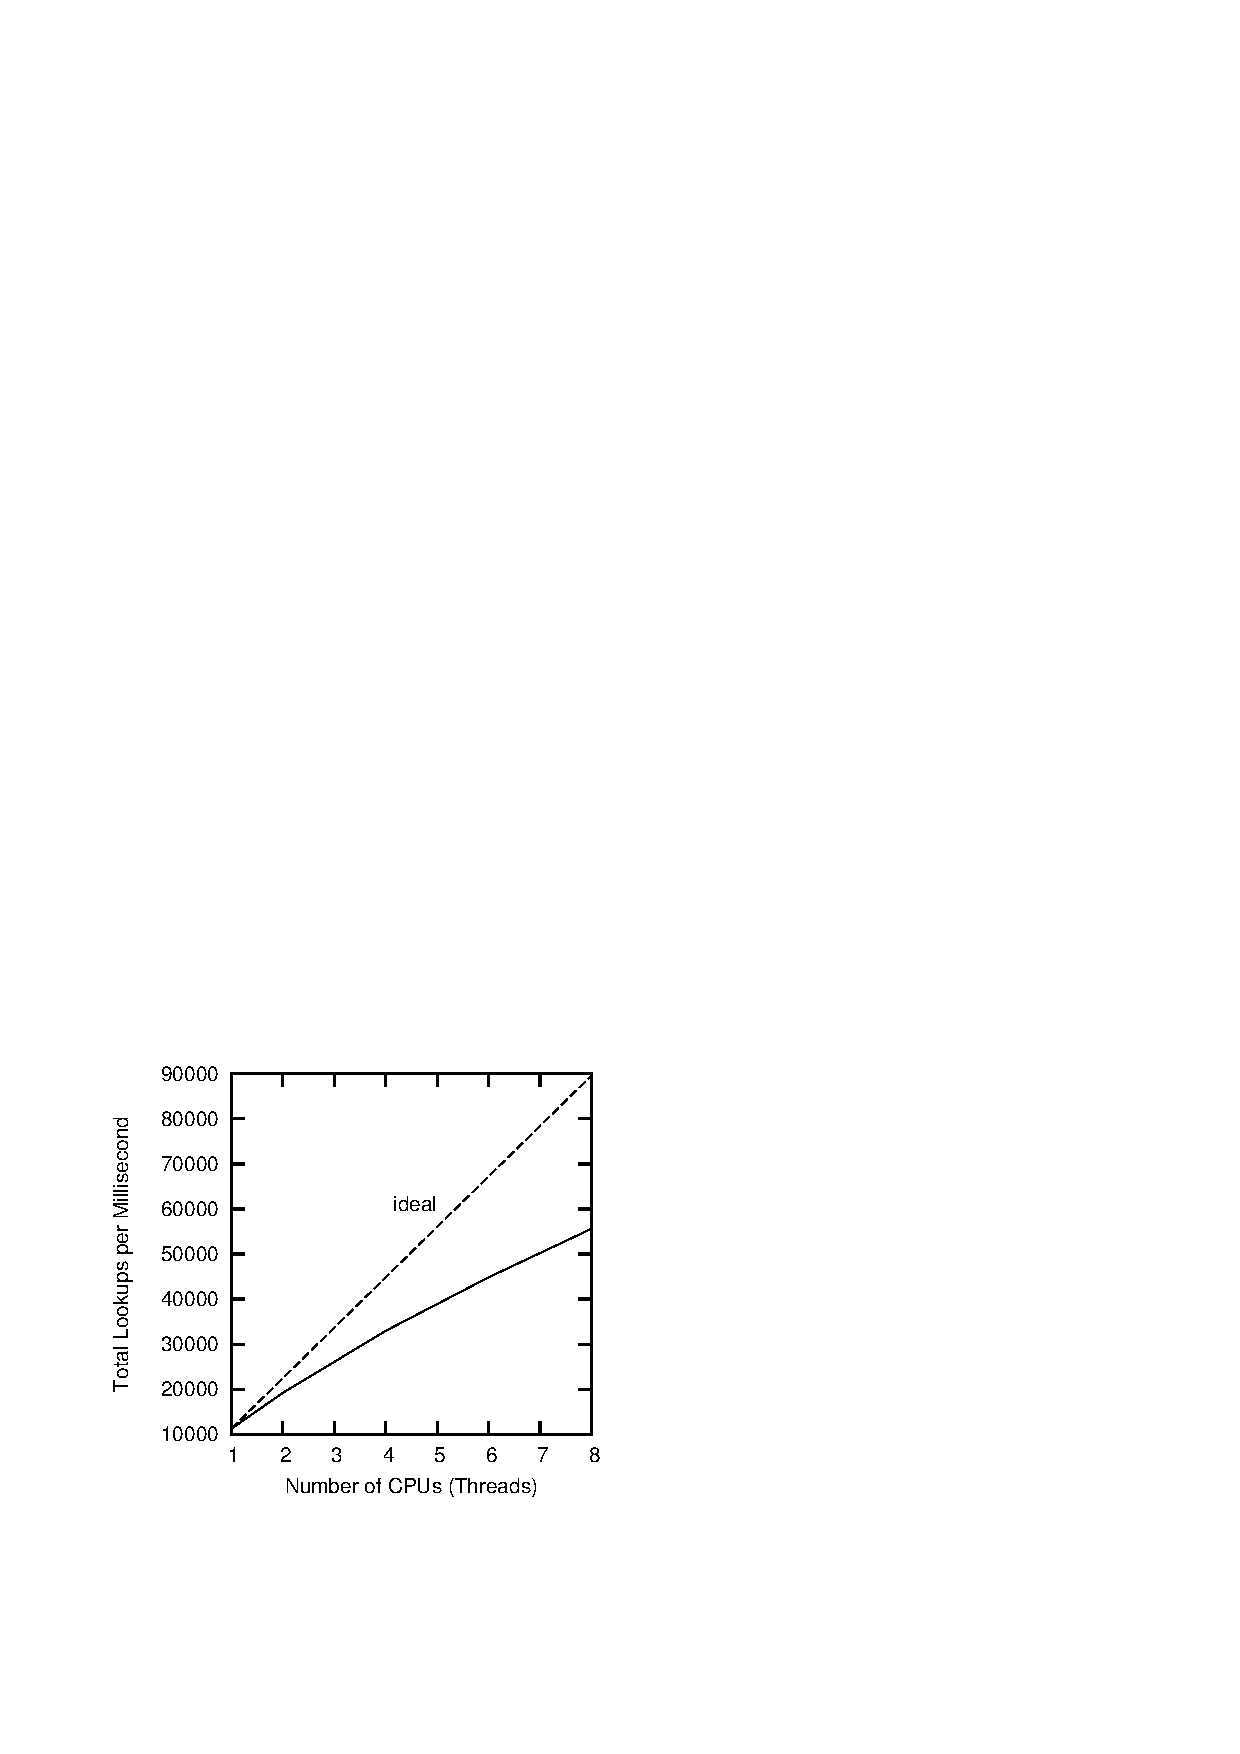
\includegraphics{datastruct/zoocpubktlin8}}
\caption{Read-Only Hash-Table Performance For Schr\"odinger's Zoo}
\label{fig:datastruct:Read-Only Hash-Table Performance For Schroedinger's Zoo}
\end{figure}

여덟개의 2\,GHz
Intel\textsuperscript\textregistered
Xeon\textsuperscript\textregistered
CPU 를 사용한 시스템에서 bucket 별 락을 사용하며 1024개 bucket 을 가진 해시
테이블을 사용한 성능 결과가
Figure~\ref{fig:datastruct:Read-Only Hash-Table Performance For Schroedinger's Zoo}
에 있습니다.
이 성능은 거의 선형적으로 증가합니다만, 8개의 CPU 만 사용함에도 이상적인 성능
기준의 절반을 넘지 못합니다.
이는 락 획득과 해제가 하나의 CPU 에서는 캐시 미스를 내지 않지만, 두개 이상의
CPU 에서는 캐시 미스를 내기 때문입니다.
\iffalse

The performance results for an eight-CPU 2\,GHz
Intel\mytextregistered\
Xeon\mytextregistered\
system using a bucket-locked hash table with 1024 buckets are shown in
Figure~\ref{fig:datastruct:Read-Only Hash-Table Performance For Schroedinger's Zoo}.
The performance does scale nearly linearly, but is not much more than half
of the ideal performance level, even at only eight CPUs.
Part of this shortfall is due to the fact that the lock acquisitions and
releases incur no cache misses on a single CPU, but do incur misses
on two or more CPUs.
\fi

\begin{figure}[tb]
\centering
\resizebox{2.5in}{!}{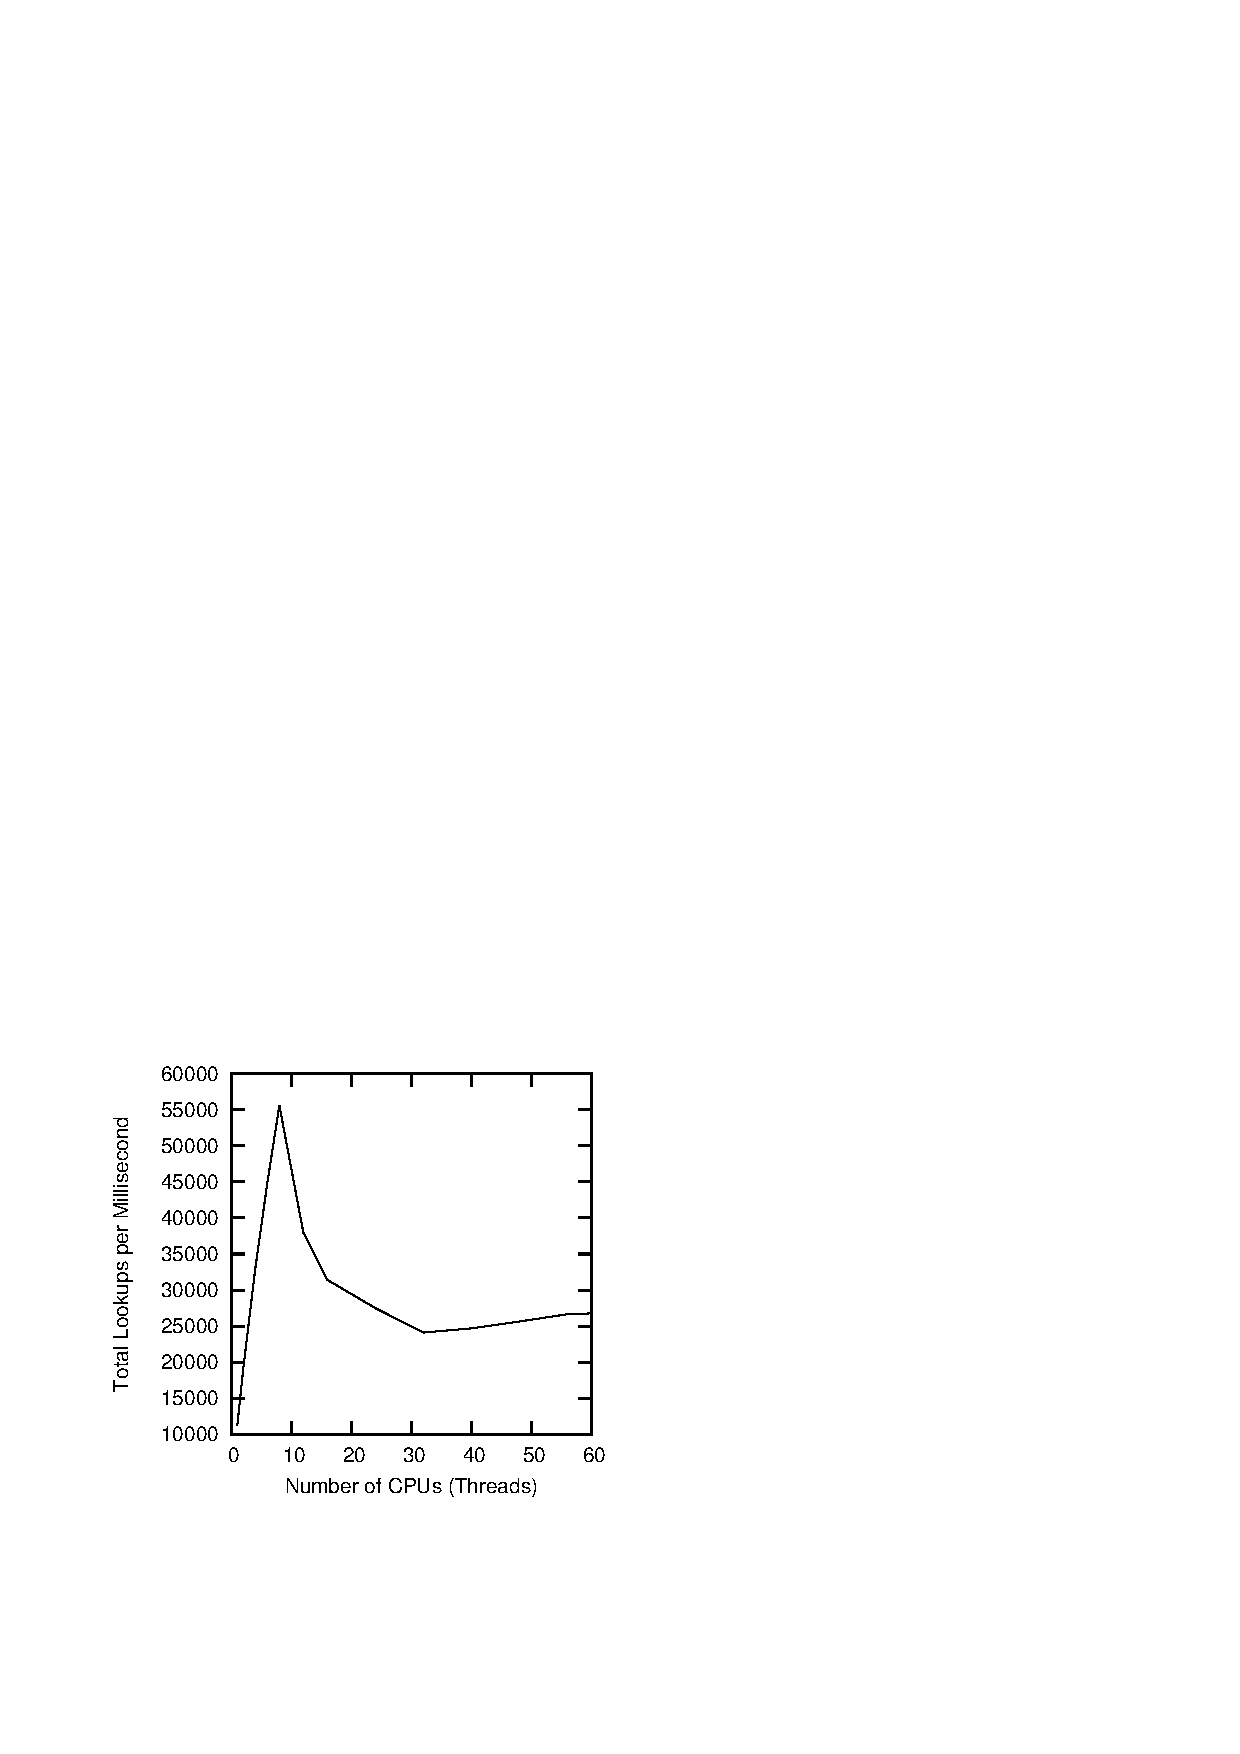
\includegraphics{datastruct/zoocpubktlin}}
\caption{Read-Only Hash-Table Performance For Schr\"odinger's Zoo, 60 CPUs}
\label{fig:datastruct:Read-Only Hash-Table Performance For Schroedinger's Zoo, 60 CPUs}
\end{figure}

그리고 CPU 의 수가 커져갈수록 상황은 더 나빠져가는데, 이를
Figure~\ref{fig:datastruct:Read-Only Hash-Table Performance For Schroedinger's Zoo, 60 CPUs}
가 보이고 있습니다.
여기선 이상적 성능을 위한 선을 추가적으로 보일 필요도 없습니다: 9개 이상의 CPU
에서의 성능은 끔찍합니다.
이는 적당한 수의 CPU 이상으로 CPU 를 늘리는 것의 위험성을 분명하게 강조합니다.
\iffalse

And things only get worse with larger number of CPUs, as can be seen in
Figure~\ref{fig:datastruct:Read-Only Hash-Table Performance For Schroedinger's Zoo, 60 CPUs}.
We do not need an additional line to show ideal performance: The performance
for nine CPUs and beyond is worse than abysmal.
This clearly underscores the dangers of extrapolating performance from a
modest number of CPUs.
\fi

물론, 이렇게 성능이 떨어지는 것은 bucket 의 수가 부족해서일 수도 있습니다.
일단, 우리는 각 bucket 이 cache line 에 맞아 떨어지도록 패딩을 넣지 않았고,
따라서 하나의 캐시 라인에 여러 bucket 들이 존재할 겁니다.
이로 인해 9개 CPU 에서부터 캐시 쓰래싱이 시작되었을 수 있습니다.
당연하게도 이는 bucket 의 수를 늘리는 것으로 테스트 해볼 수 있을 겁니다.
\iffalse

Of course, one possible reason for the collapse in performance might be
that more hash buckets are needed.
After all, we did not pad each hash bucket to a full cache line, so
there are a number of hash buckets per cache line.
It is possible that the resulting cache-thrashing comes into play at
nine CPUs.
This is of course easy to test by increasing the number of hash buckets.
\fi

\QuickQuiz{}
	단순히 bucket 들의 수를 늘리는 대신에 이미 있는 bucket 들을 캐시에 정렬
	시키는게 더 낫지 않을까요?
	\iffalse

	Instead of simply increasing the number of hash buckets,
	wouldn't it be better to cache-align the existing hash buckets?
	\fi
\QuickQuizAnswer{
	이에 대한 답은 상당히 많은 것들에 의존적입니다.
	만약 해시 테이블이 bucket 마다 많은 수의 원소를 가지고 있었다면, bucket
	들의 수를 늘리는게 분명 나을 겁니다.
	한편으로는, 만약 해시 테이블에 가해지는 로드가 적었다면, 이에 대한 답은
	하드웨어, 해시 함수의 효율성, 그리고 워크로드에 의존적일 겁니다.
	관심있는 독자들은 실험을 해보시기 바랍니다.
	\iffalse

	The answer depends on a great many things.
	If the hash table has a large number of elements per bucket, it
	would clearly be better to increase the number of hash buckets.
	On the other hand, if the hash table is lightly loaded,
	the answer depends on the hardware, the effectiveness of the
	hash function, and the workload.
	Interested readers are encouraged to experiment.
	\fi
} \QuickQuizEnd


\begin{figure}[tb]
\centering
\resizebox{2.5in}{!}{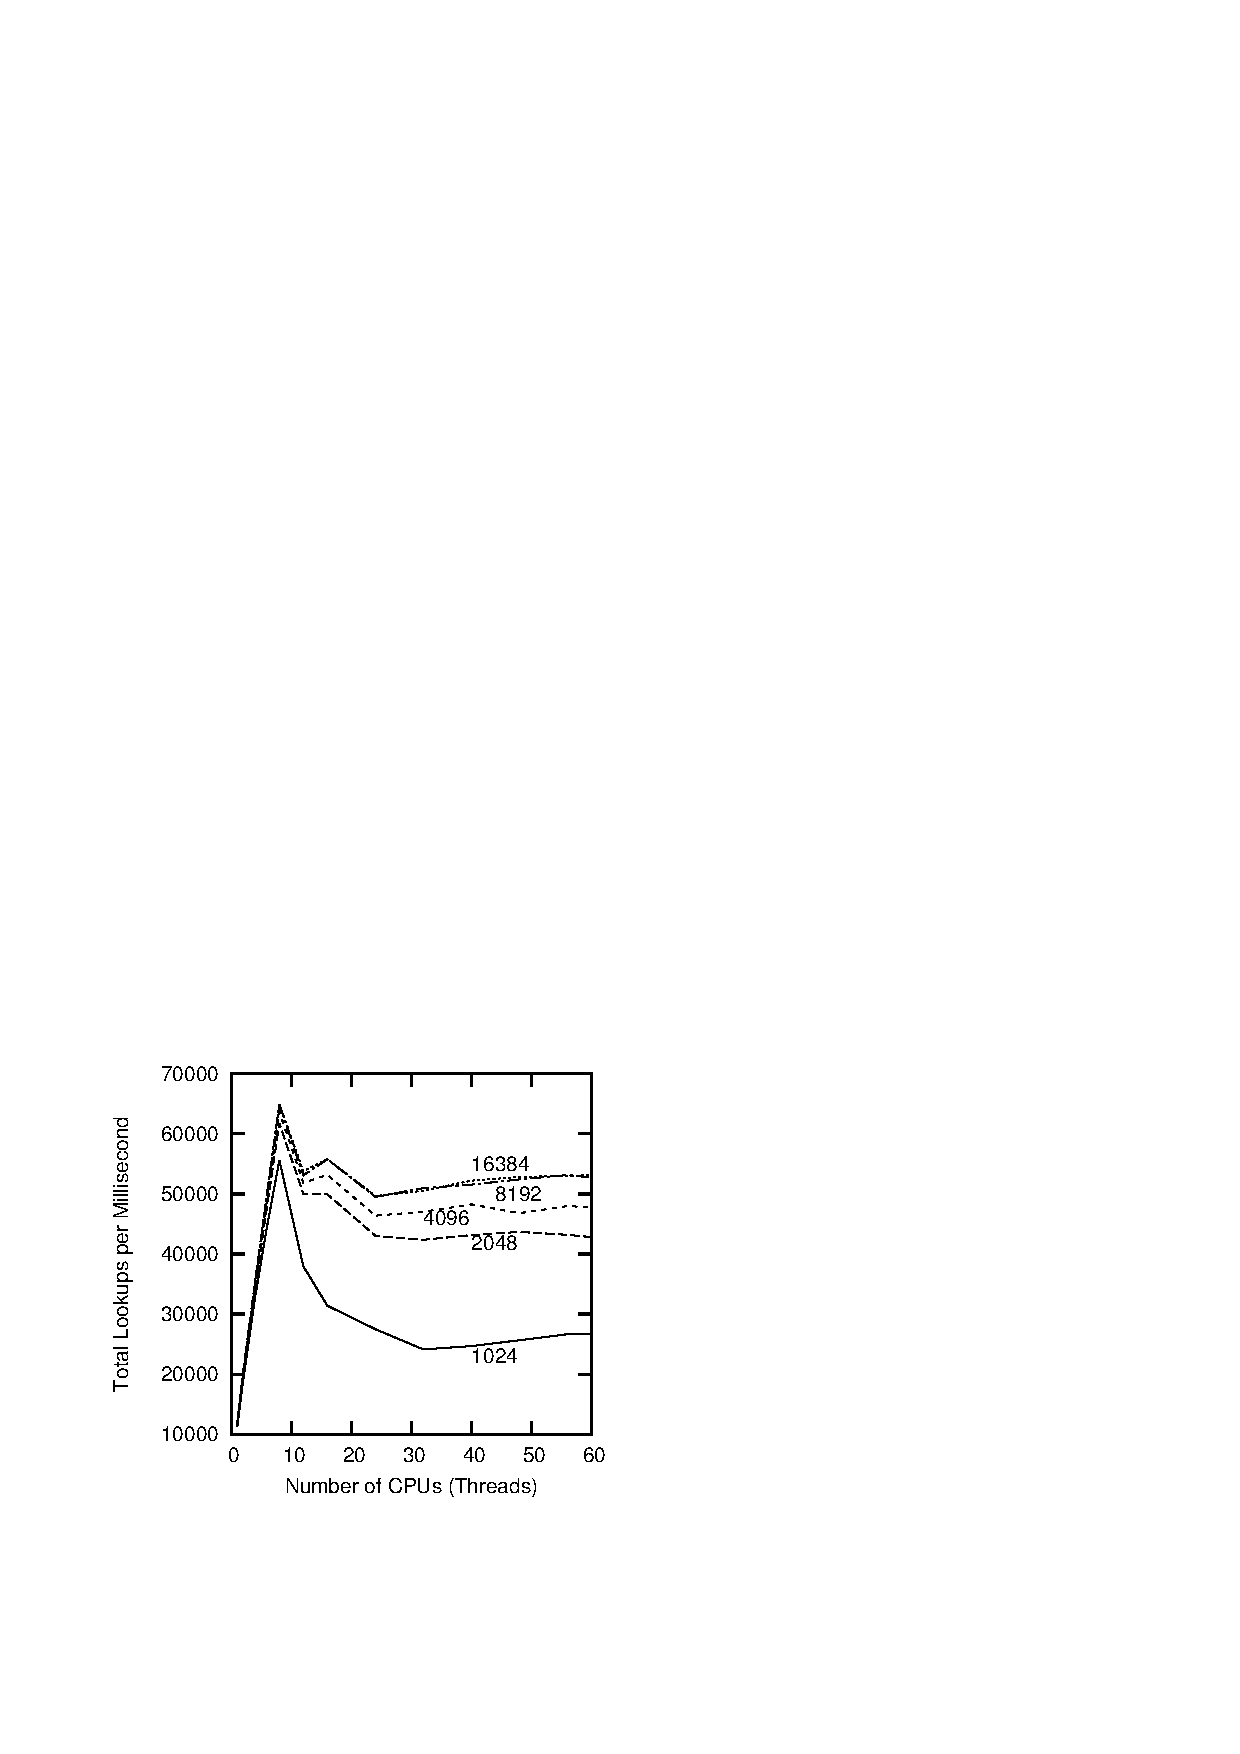
\includegraphics{datastruct/zoocpubktsizelin}}
\caption{Read-Only Hash-Table Performance For Schr\"odinger's Zoo, Varying Buckets}
\label{fig:datastruct:Read-Only Hash-Table Performance For Schroedinger's Zoo, Varying Buckets}
\end{figure}

하지만,
Figure~\ref{fig:datastruct:Read-Only Hash-Table Performance For Schroedinger's Zoo, Varying Buckets},
에서 볼 수 있듯이, bucket 들의 수를 늘리는 것이 실제로 성능을 어느정도
증가시키기는 하지만, 확장성은 여전히 끔찍합니다.
특히, 아홉개 이상의 CPU 들에서는 여전히 현격한 성능 저하를 볼 수 있습니다.
더 나아가서, 8,192 개 bucket 에서 16,384 개의 bucket 으로 넘어가는것부터는
더이상 성능이 늘어나지도 않습니다.
분명 뭔가가 잘못되어 있습니다.
\iffalse

However, as can be seen in
Figure~\ref{fig:datastruct:Read-Only Hash-Table Performance For Schroedinger's Zoo, Varying Buckets},
although increasing the number of buckets does increase performance somewhat,
scalability is still abysmal.
In particular, we still see a sharp dropoff at nine CPUs and beyond.
Furthermore, going from 8,192 buckets to 16,384 buckets produced almost
no increase in performance.
Clearly something else is going on.
\fi

문제는 이 시스템이
Figure~\ref{fig:datastruct:NUMA Topology of System Under Test} 에 보인 것처럼
CPU~0-7 과 32-39 가 첫번째 소켓에 위치하는 멀티 소켓 시스템이라는 점입니다.
따라서, 처음 여덟개 CPU 에 국한되어 돌아가는 테스트는 상당히 잘 동작하지만,
소켓~0 의 CPU~0-7 과 소켓~1 의 CPU~8 이 관여되는 테스트에서는 데이터를 소켓
너머로 주고받는 오버헤드가 생겨납니다.
이는
Section~\ref{sec:cpu:Hardware System Architecture} 에서 보인 것처럼, 성능을
상당히 저하시킬 수 있습니다.
요약해서, 커다란 멀티 소켓 시스템에서는 완전한 파티셔닝에 더해서 메모리 참조의
높은 로컬리티를 필요로 합니다.
\iffalse

The problem is that this is a multi-socket system, with CPUs~0-7
and~32-39 mapped to the first socket as shown in
Figure~\ref{fig:datastruct:NUMA Topology of System Under Test}.
Test runs confined to the first eight CPUs therefore perform quite
well, but tests that involve socket~0's CPUs~0-7 as well as
socket~1's CPU~8 incur the overhead of passing data across
socket boundaries.
This can severely degrade performance, as was discussed in
Section~\ref{sec:cpu:Hardware System Architecture}.
In short, large multi-socket systems require good locality of reference
in addition to full partitioning.
\fi

\QuickQuiz{}
	Schr\"odinger 의 동물원 어플리케이션의 소켓을 넘어가면서 보이는 음의
	확장성을 가지고 생각해보면, 어플리케이션의 복사본을 여럿 만들어서
	각각의 복사본이 전체 동물의 부분집합만을 가지고 하나의 소켓 위에서만
	각자 돌도록 하는 건 어떨까요?
	\iffalse

	Given the negative scalability of the Schr\"odinger's
	Zoo application across sockets, why not just run multiple
	copies of the application, with each copy having a subset
	of the animals and confined to run on a single socket?
	\fi
\QuickQuizAnswer{
	그렇게 해볼 수 있습니다!
	사실, 이 아이디어를 커다란 클러스터 시스템으로 확장할 수도 있는데, 각
	어플리케이션 복사본을 클러스터의 각 노드에 수행시키는 형식으로
	말입니다.
	이 방법은 ``sharding'' 이라 불리며, 실제로 커다란 웹 기반의 상점에서
	상당히 많이 사용되는
	방법입니다~\cite{DeCandia:2007:DAH:1323293.1294281}.

	하지만, 멀티소켓 시스템에서 소켓별로 분할을 하려 한다면, 별개의 더 작고
	싼 단일 소켓 시스템들을 사서 각각의 데이터베이스 조각을 그 각각의
	시스템에서 수행시키는게 어떻겠어요?
	\iffalse

	You can do just that!
	In fact, you can extend this idea to large clustered systems,
	running one copy of the application on each node of the cluster.
	This practice is called ``sharding'', and is heavily used in
	practice by large web-based
	retailers~\cite{DeCandia:2007:DAH:1323293.1294281}.

	However, if you are going to shard on a per-socket basis within
	a multisocket system, why not buy separate smaller and cheaper
	single-socket systems, and then run one shard of the database
	on each of those systems?
	\fi
} \QuickQuizEnd

지금까지 논의된 Schr\"odinger's-zoo 수행의 한가지 핵심적 특성은 이것들이 모두
읽기만 했다는 것입니다.
이는 락 획득이 초래한 캐시 미스들로 인해 발생한 성능 하락을 더욱 심하게
만듭니다.
이 아래에 깔려 있는 해시 테이블 자체에 대해 업데이트를 하지 않더라도, 메모리에
쓰기를 하기 위한 비용은 여전히 지불되고 있는 것입니다.
물론, 이 해시 테이블이 절대 업데이트 되지 않는다면, 상호 배타성을 완전히 제거할
수 있을 겁니다.
이 방법은 상당히 단순하고, 따라서 독자들의 연습으로 남겨두겠습니다.
하지만 결국은 일어나는 업데이트가 있다 하더라도, 쓰기를 막는 것은 캐시 미스를
막을 것이고, 이는 읽기가 대부분인 데이터의 복사본을 모든 캐시에 만들어두는
것으로 메모리 참조의 로컬리티를 높여줄 수 있을 것입니다.

따라서 다음 섹션에서는 읽기가 대부분이지만 업데이트가 가끔씩이지만 언제든
일어날 수 있는 경우를 위한 최적화들을 알아보겠습니다.
\iffalse

One key property of the Schr\"odinger's-zoo runs discussed thus far is that
they are all read-only.
This makes the performance degradation due to lock-acquisition-induced
cache misses all the more painful.
Even though we are not updating the underlying hash table itself, we are
still paying the price for writing to memory.
Of course, if the hash table was never going to be updated, we could dispense
entirely with mutual exclusion.
This approach is quite straightforward and is left as an exercise for the
reader.
But even with the occasional update, avoiding writes avoids cache
misses, and allows the read-mostly data to be replicated across all
the caches, which in turn promotes locality of reference.

The next section therefore examines optimizations that can be carried out in
read-mostly cases where updates are rare, but could happen at any time.
\fi

\setlength\dashlinedash{1pt}
\setlength\dashlinegap{2pt}

\begin{figure}
\renewcommand*{\arraystretch}{1.2}
\footnotesize
\centering
\begin{tabular}{r|r:r:r:r:r:r:r:r|}
	Socket & \multicolumn{8}{c|}{Core} \\
	\hline
	0 &  0 &  1 &  2 &  3 &  4 &  5 &  6 &  7 \\
	\cdashline{2-9}
	  & 32 & 33 & 34 & 35 & 36 & 37 & 38 & 39 \\
	\hline
	1 &  8 &  9 & 10 & 11 & 12 & 13 & 14 & 15 \\
	\cdashline{2-9}
	  & 40 & 41 & 42 & 43 & 44 & 45 & 46 & 47 \\
	\hline
	2 & 16 & 17 & 18 & 19 & 20 & 21 & 22 & 23 \\
	\cdashline{2-9}
	  & 48 & 49 & 50 & 51 & 52 & 53 & 54 & 55 \\
	\hline
	3 & 24 & 25 & 26 & 27 & 28 & 29 & 30 & 31 \\
	\cdashline{2-9}
	  & 56 & 47 & 58 & 59 & 60 & 61 & 62 & 63 \\
	\hline
\end{tabular}
\caption{NUMA Topology of System Under Test}
\label{fig:datastruct:NUMA Topology of System Under Test}
\end{figure}

\section{Read-Mostly Data Structures}
\label{sec:datastruct:Read-Mostly Data Structures}

파티셔닝이 적용된 데이터 구조가 훌륭한 확장성을 제공할 수 있긴 하지만, NUMA
효과는 성능과 확장성 모두를 심각하게 저하시킬 수 있습니다.
더불어, 읽기 쓰레드가 쓰기 쓰레드와 배타적으로 동작해야 한다는 필요성이 읽기가
대부분인 상황에서의 성능을 저하시킬 수 있습니다.
하지만,
Section~\ref{sec:defer:Read-Copy Update (RCU)} 에서 소개된 바 있는 RCU 를
사용해서 성능과 확장성을 모두 달성할 수 있습니다.
비슷한 결과를 해저드 포인터를 이용해서 얻을 수도 있는데(\path{hazptr.c}), 이는
이 섹션의 성능 결과에서 보여질 겁니다~\cite{McKenney:2013:SDS:2483852.2483867}.
\iffalse

Although partitioned data structures can offer excellent scalability,
NUMA effects can result in severe degradations of both performance and
scalability.
In addition,
the need for readers to exclude writers can degrade performance in
read-mostly situations.
However, we can achieve both performance and scalability by using
RCU, which was introduced in
Section~\ref{sec:defer:Read-Copy Update (RCU)}.
Similar results can be achieved using hazard pointers
(\path{hazptr.c})~\cite{MagedMichael04a}, which will be included in
the performance results shown in this
section~\cite{McKenney:2013:SDS:2483852.2483867}.
\fi

\subsection{RCU-Protected Hash Table Implementation}
\label{sec:datastruct:RCU-Protected Hash Table Implementation}

\begin{listing}[tb]
\input{CodeSamples/datastruct/hash/hash_bkt_rcu@lock_unlock.fcv}
\caption{RCU-Protected Hash-Table Read-Side Concurrency Control}
\label{lst:datastruct:RCU-Protected Hash-Table Read-Side Concurrency Control}
\end{listing}

Bucket 별 락킹을 사용하는 RCU 로 보호되는 해시 테이블에서, 업데이트 쓰레드는
Section~\ref{sec:datastruct:Partitionable Data Structures} 에서 설명된 것과
똑같이 락킹을 사용하지만 읽기 쓰레드는 RCU 를 사용합니다.
데이터 구조는
Listing~\ref{lst:datastruct:Hash-Table Data Structures} 에서 보인 것과 똑같이
남아 있고,
\co{HASH2BKT()}, \co{hashtab_lock()}, 그리고 \co{hashtab_unlock()} 함수들은
Listing~\ref{lst:datastruct:Hash-Table Mapping and Locking} 에서 보인 것과
똑같습니다.
하지만, 읽기 쓰레드는
Listing~\ref{lst:datastruct:RCU-Protected Hash-Table Read-Side Concurrency Control}
에 보인 것과 같이
\co{hashtab_lock_lookup()} 와 \co{hashtab_unlock_lookup()} 로 둘러싸인 더
가벼운 동시성 제어 방법을 사용할 겁니다.
\iffalse

For an RCU-protected hash table with per-bucket locking,
updaters use locking exactly as described in
Section~\ref{sec:datastruct:Partitionable Data Structures},
but readers use RCU.
The data structures remain as shown in
Listing~\ref{lst:datastruct:Hash-Table Data Structures},
and the \co{HASH2BKT()}, \co{hashtab_lock()}, and \co{hashtab_unlock()}
functions remain as shown in
Listing~\ref{lst:datastruct:Hash-Table Mapping and Locking}.
However, readers use the lighter-weight concurrency-control embodied
by \co{hashtab_lock_lookup()} and \co{hashtab_unlock_lookup()}
shown in
Listing~\ref{lst:datastruct:RCU-Protected Hash-Table Read-Side Concurrency Control}.
\fi

\begin{listing}[tb]
\input{CodeSamples/datastruct/hash/hash_bkt_rcu@lookup.fcv}
\caption{RCU-Protected Hash-Table Lookup}
\label{lst:datastruct:RCU-Protected Hash-Table Lookup}
\end{listing}

Listing~\ref{lst:datastruct:RCU-Protected Hash-Table Lookup} 는 bucket 별
락킹을 사용하며 RCU 로 보호되는 해시 테이블에 사용되는 \co{hashtab_lookup()}
함수를 보입니다.
이 함수는 \co{cds_list_for_each_entry()} 가 \co{cds_list_for_each_entry_rcu()}
로 바뀌었다는 점을 제외하고는
Listing~\ref{lst:datastruct:Hash-Table Lookup} 에서 보인 버전과 동일합니다.
이것들 둘 다 \co{htb->htb_head} 로 레퍼런스되는 해시 체인을 따라간다는 점에서는
동일합니다만 \co{cds_list_for_each_entry_rcu()} 는 추가적으로, 동시의 삽입이
존재하는 경우에 올바른 메모리 액세스 순서를 강제합니다:
순수한 bucket 별 락킹 사용 구현과 달리, RCU 로 보호되는 구현에서는 검색 작업이
삽입이나 삭제 작업과 동시에 수행되는 것이 허용되고, RCU 를 신경쓰는 기능인
\co{cds_list_for_each_entry_rcu()} 와 같은 것들은 이 추가적 동시성을 올바로
제어할 것이 요구됩니다.
또한 \co{hashtab_lookup()} 의 호출자는 RCU read-side 크리티컬 섹션 안에 있어야
한다는 점을 알아둬야 하는데, 예를 들어 호출자는 \co{hashtab_lookup()} 을
호출하기 전에 \co{hashtab_lock_lookup()} 을 호출해야만 합니다 (그리고 나중에는
당연히 \co{hashtab_unlock_lookup()} 을 호출해야겠죠).
\iffalse

Listing~\ref{lst:datastruct:RCU-Protected Hash-Table Lookup}
shows \co{hashtab_lookup()} for the RCU-protected per-bucket-locked
hash table.
This is identical to that in
Listing~\ref{lst:datastruct:Hash-Table Lookup}
except that \co{cds_list_for_each_entry()} is replaced
by \co{cds_list_for_each_entry_rcu()}.
Both of these primitives sequence down the hash chain referenced
by \co{htb->htb_head} but \co{cds_list_for_each_entry_rcu()} also
correctly enforces memory ordering in case of concurrent insertion.
This is an important difference between these two hash-table implementations:
Unlike the pure per-bucket-locked implementation, the RCU protected
implementation allows lookups to run concurrently with insertions
and deletions, and RCU-aware primitives like
\co{cds_list_for_each_entry_rcu()} are required to correctly handle
this added concurrency.
Note also that \co{hashtab_lookup()}'s caller must be within an
RCU read-side critical section, for example, the caller must invoke
\co{hashtab_lock_lookup()} before invoking \co{hashtab_lookup()}
(and of course invoke \co{hashtab_unlock_lookup()} some time afterwards).
\fi

\QuickQuiz{}
	하지만 해시 테이블의 원소가 검색과 동시에 삭제될 수가 있다면, 그 말은
	검색 기능은 검색된 직후에 삭제된 원소로의 레퍼런스를 리턴할 수도 있다는
	의미 아닌가요?
	\iffalse

	But if elements in a hash table can be deleted concurrently
	with lookups, doesn't that mean that a lookup could return
	a reference to a data element that was deleted immediately
	after it was looked up?
	\fi
\QuickQuizAnswer{
	네, 그럴 수 있습니다!
	이게 왜 \co{hashtab_lookup()} 이 RCU read-side 크리티컬 섹션 안에서
	호출되어야만 하는지에 대한 이유이고, 왜 \co{hashtab_add()} 와
	\co{hashtab_del()} 역시 RCU 를 신경쓰는 리스트 조작 기능을 사용해야
	하는가에 대한 이유입니다.
	마지막으로, 이게 바로 \co{hashtab_del()} 가 삭제한 원소를 메모리에서
	해제시키기 전에 (ex: \co{sychronize_rcu()} 를 호출해서) grace period 를
	기다려야 하는지에 대한 이유입니다.
	\iffalse

	Yes it can!
	This is why \co{hashtab_lookup()} must be invoked within an
	RCU read-side critical section, and it is why
	\co{hashtab_add()} and \co{hashtab_del()} must also use
	RCU-aware list-manipulation primitives.
	Finally, this is why the caller of \co{hashtab_del()} must
	wait for a grace period (e.g., by calling \co{synchronize_rcu()})
	before freeing the deleted element.
	\fi
} \QuickQuizEnd

\begin{listing}[tb]
\input{CodeSamples/datastruct/hash/hash_bkt_rcu@add_del.fcv}
\caption{RCU-Protected Hash-Table Modification}
\label{lst:datastruct:RCU-Protected Hash-Table Modification}
\end{listing}

Listing~\ref{lst:datastruct:RCU-Protected Hash-Table Modification} 는
\co{hashtab_add()} 와 \co{hashtab_del()} 함수를 보이는데, 둘 다
Listing~\ref{lst:datastruct:Hash-Table Modification} 에서 보인 RCU 를 사용하지
않는 해시 테이블에서의 같은 기능을 하는 것들과 상당히 비슷합니다.
\co{hashtab_add()} 함수는 검색되고 있는 도중에 동시에 해시 테이블에 더해지는
원소의 경우에 대해 올바른 순서를 강제하기 위해서 \co{cds_list_add()} 대신에
\co{cds_list_add_rcu()} 함수를 사용합니다.
\co{hashtab_del()} 함수는 삭제되기 직전에 검색되는 원소의 경우를 위해서
\co{cds_list_del_init()} 대신에 \co{cds_list_del_rcu()} 함수를 사용합니다.
\co{cds_list_del_init()} 와 달리, \co{cds_list_del_rcu()} 는 다음 원소로의
포인터를 온전하게 남겨두어서 \co{hashtab_lookup()} 이 삭제된 원소의 다음
원소로도 갈 수 있게 해줍니다.

물론, \co{hashtab_del()} 을 호출한 후에, 호출자는 이번에 삭제한 원소의 메모리를
해제하거나 재사용하기 전에 (\co{synchronize_rcu()} 를 호출하거나 하는 식으로)
하나의 RCU grace period 를 기다려야만 합니다.
\iffalse

Listing~\ref{lst:datastruct:RCU-Protected Hash-Table Modification}
shows \co{hashtab_add()} and \co{hashtab_del()}, both of which
are quite similar to their counterparts in the non-RCU hash table
shown in
Listing~\ref{lst:datastruct:Hash-Table Modification}.
The \co{hashtab_add()} function uses \co{cds_list_add_rcu()} instead
of \co{cds_list_add()} in order to ensure proper ordering when
an element is added to the hash table at the same time that it is
being looked up.
The \co{hashtab_del()} function uses \co{cds_list_del_rcu()} instead
of \co{cds_list_del_init()} to allow for the case where an element is
looked up just before it is deleted.
Unlike \co{cds_list_del_init()}, \co{cds_list_del_rcu()} leaves the
forward pointer intact, so that \co{hashtab_lookup()} can traverse
to the newly deleted element's successor.

Of course, after invoking \co{hashtab_del()}, the caller must wait for
an RCU grace period (e.g., by invoking \co{synchronize_rcu()}) before
freeing or otherwise reusing the memory for the newly deleted element.
\fi

\subsection{RCU-Protected Hash Table Performance}
\label{sec:datastruct:RCU-Protected Hash Table Performance}

\begin{figure}[tb]
\centering
\resizebox{2.5in}{!}{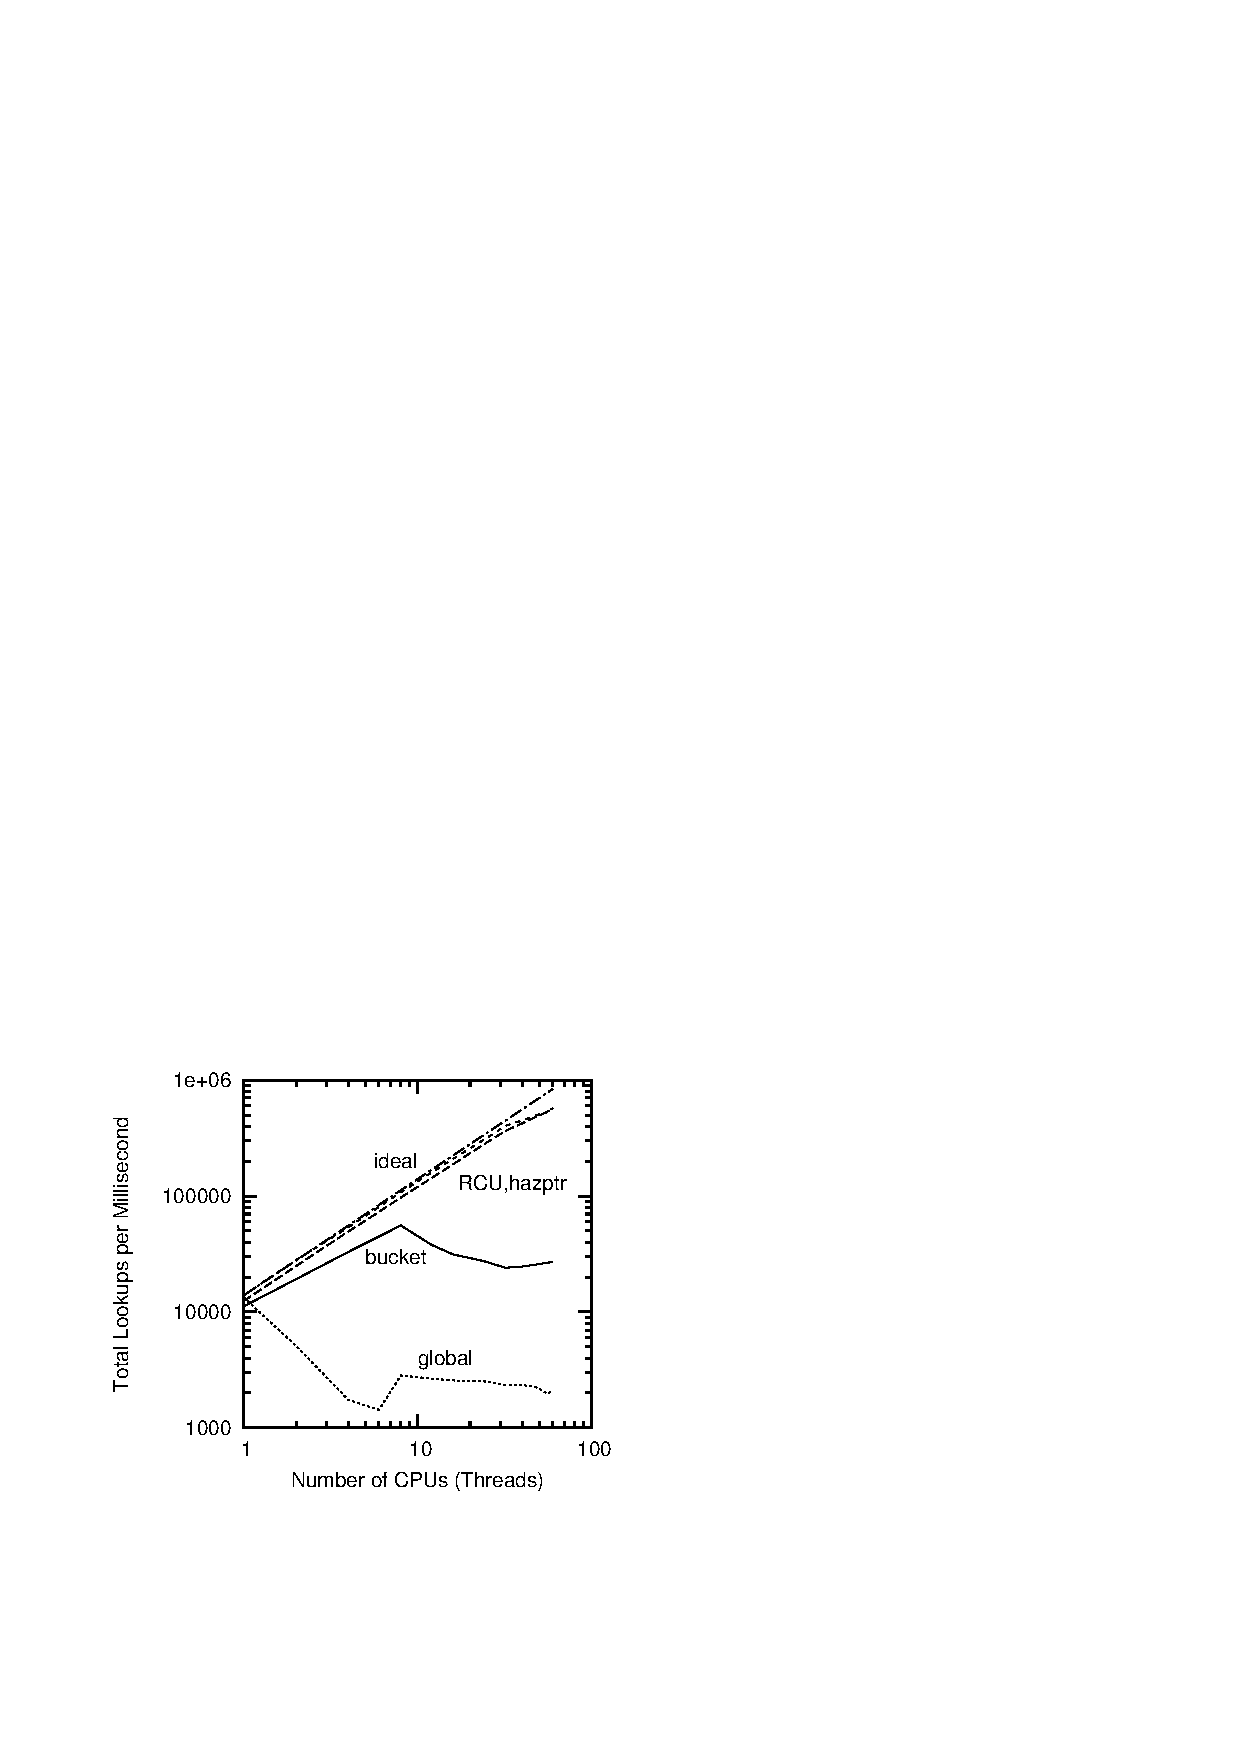
\includegraphics{datastruct/zoocpu}}
\caption{Read-Only RCU-Protected Hash-Table Performance For Schr\"odinger's Zoo}
\label{fig:datastruct:Read-Only RCU-Protected Hash-Table Performance For Schroedinger's Zoo}
\end{figure}

Figure~\ref{fig:datastruct:Read-Only RCU-Protected Hash-Table Performance For Schroedinger's Zoo}
는 RCU 로 보호되는 버전과 해저드 포인터로 보호되는 버전의 해시 테이블들의
읽기만 일어나는 상황에서의 성능을 앞 섹션에서 본 bucket 별 락킹 사용 구현
버전과 비교해 보이고 있습니다.
볼 수 있듯이, RCU 와 해저드 포인터 둘 다 큰 수의 쓰레드들 에서는 NUMA 영향을
받기는 하지만 이상적인 경우에 가까운 성능과 확장성을 보이고 있습니다.
테이블 전체를 하나의 락으로 보호하는 구현의 결과도 보이고 있는데, 그런
상황에서의 성능은 기대된 대로 bucket 별 락킹 구현 버전에 비해서조차도 나쁨을 볼
수 있습니다.
RCU 는 해저드 포인터보다 아주 약간 좋은 성능을 보이기는 하지만, 그 차이는 이
로그스케일 그림에서는 거의 보이지도 않을 정도입니다.
\iffalse

Figure~\ref{fig:datastruct:Read-Only RCU-Protected Hash-Table Performance For Schroedinger's Zoo}
shows the read-only performance of RCU-protected and hazard-pointer-protected
hash tables against the previous section's per-bucket-locked implementation.
As you can see, both RCU and hazard pointers achieve near-ideal performance
and scalability despite the larger numbers of threads and the NUMA effects.
Results from a globally locked implementation are also shown, and as expected
the results are even worse than those of the per-bucket-locked implementation.
RCU does slightly better than hazard pointers, but the difference is not
readily visible in this log-scale plot.
\fi

\begin{figure}[tb]
\centering
\resizebox{2.5in}{!}{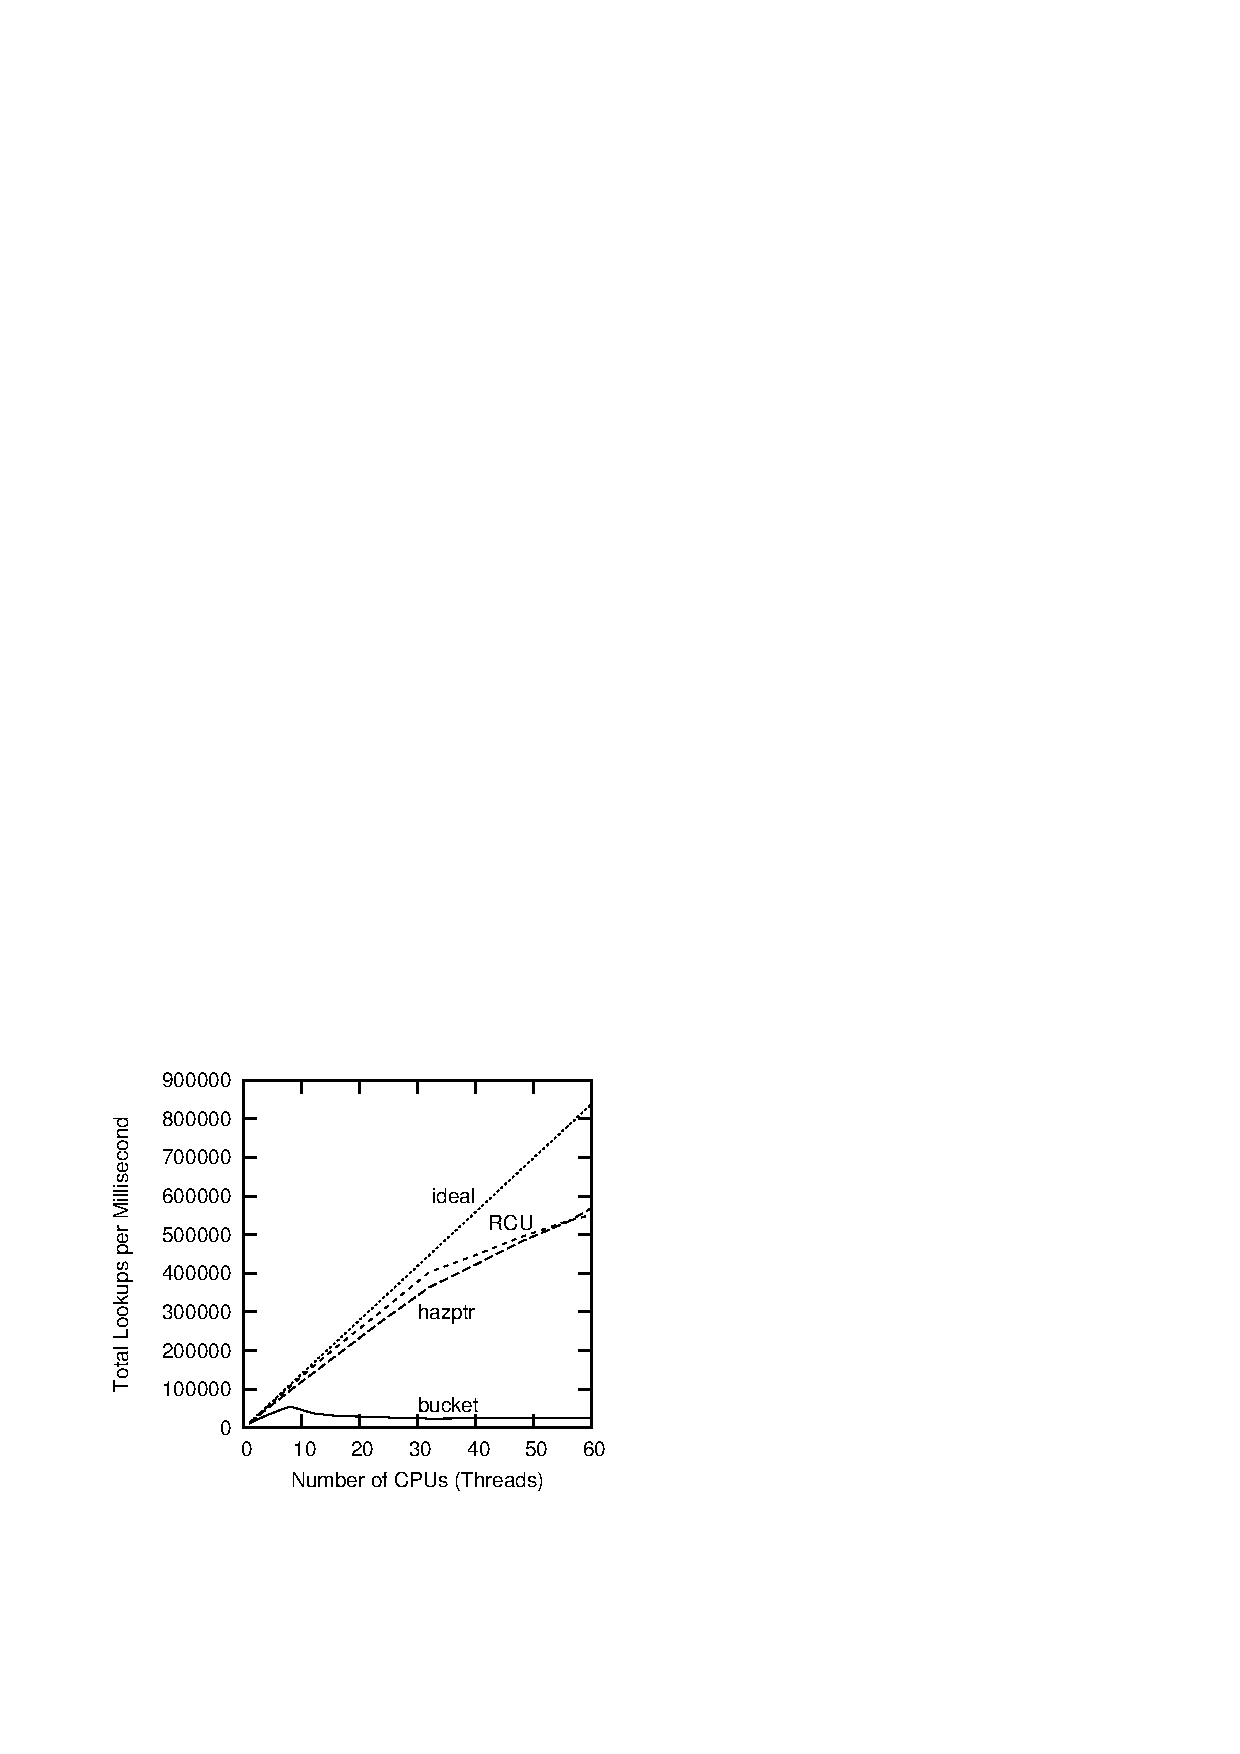
\includegraphics{datastruct/zoocpulin}}
\caption{Read-Only RCU-Protected Hash-Table Performance For Schr\"odinger's Zoo, Linear Scale}
\label{fig:datastruct:Read-Only RCU-Protected Hash-Table Performance For Schroedinger's Zoo, Linear Scale}
\end{figure}

Figure~\ref{fig:datastruct:Read-Only RCU-Protected Hash-Table Performance For Schroedinger's Zoo, Linear Scale}
는 같은 데이터를 로그스케일이 아닌 리니어스케일 (linear scale) 로 보입니다.
여기서는 테이블 전체를 하나의 락으로 보호하는 구현의 경우는 x 축에 붙어버려
제대로 볼수가 없지만, RCU 와 해저드 포인터 사이의 상대적 성능 차이를 좀 더
분간할 수 있습니다.
둘 다 32 CPU 를 넘어가면서 성능 증가정도가 떨어지기 시작하는 걸 볼 수 있는데,
이는 하드웨어 멀티쓰레딩 때문입니다.
32개 이하의 CPU 에서, 각각의 쓰레드는 각각의 코어를 갖고 있습니다.
이 버전에서, RCU 는 해저드 포인터보다 좋은 성능을 보이는데 이는 해저드 포인터의
read-side 메모리 배리어가 해당 코어 내에서의 시간을 잡아먹기 때문입니다.
요약하자면, RCU 는 하나의 하드웨어 쓰레드를 가지고 있을 때에는 해저드
포인터보다 코어를 더 잘 활용합니다.
\iffalse

Figure~\ref{fig:datastruct:Read-Only RCU-Protected Hash-Table Performance For Schroedinger's Zoo, Linear Scale}
shows the same data on a linear scale.
This drops the global-locking trace into the x-axis, but allows the
relative performance of RCU and hazard pointers to be more readily
discerned.
Both show a change in slope at 32 CPUs, and this is due to hardware
multithreading.
At 32 and fewer CPUs, each thread has a core to itself.
In this regime, RCU does better than does hazard pointers because
hazard pointers's read-side memory barriers result in dead time within
the core.
In short, RCU is better able to utilize a core from a single hardware
thread than is hazard pointers.
\fi

이 상황은 32개보다 많은 CPU 들의 상황에서 변합니다.
RCU 는 각 코어의 반이 넘는 리소스를 하나의 하드웨어 쓰레드에서 사용하므로, RCU
를 수행하는 코어 각각에 두개의 하드웨어 쓰레드가 존재하게 되면 그 성능 이득이
상대적으로 적어지게 됩니다.
해저드 포인터의 성능 그림에서의 경사도 역시 32 CPU 를 넘어서면서 줄어듭니다만,
RCU 에 비해서는 좀 덜 극적으로 줄어들고 있는데, 이는 두번째 하드웨어 쓰레드는
첫번째 하드웨어 쓰레드가 메모리 배리어 대기시간으로 멈춰서 있는 사이의 시간을
활용할 수 있기 때문입니다.
뒤의 섹션에서 보게 되겠지만, 하드웨어 포인터의 두번째 하드웨어 쓰레드
상황에서의 이득은 워크로드의 특성에 종속적입니다.
\iffalse

This situation changes above 32 CPUs.
Because RCU is using more than half of each core's resources from a
single hardware thread, RCU gains relatively little benefit from the
second hardware thread in each core.
The slope of hazard pointers's trace also decreases at 32 CPUs, but
less dramatically,
because the second hardware thread is able to fill in the time
that the first hardware thread is stalled due to memory-barrier latency.
As we will see in later sections, hazard pointers's second-hardware-thread
advantage depends on the workload.
\fi

\begin{figure}[tb]
\centering
\resizebox{2.5in}{!}{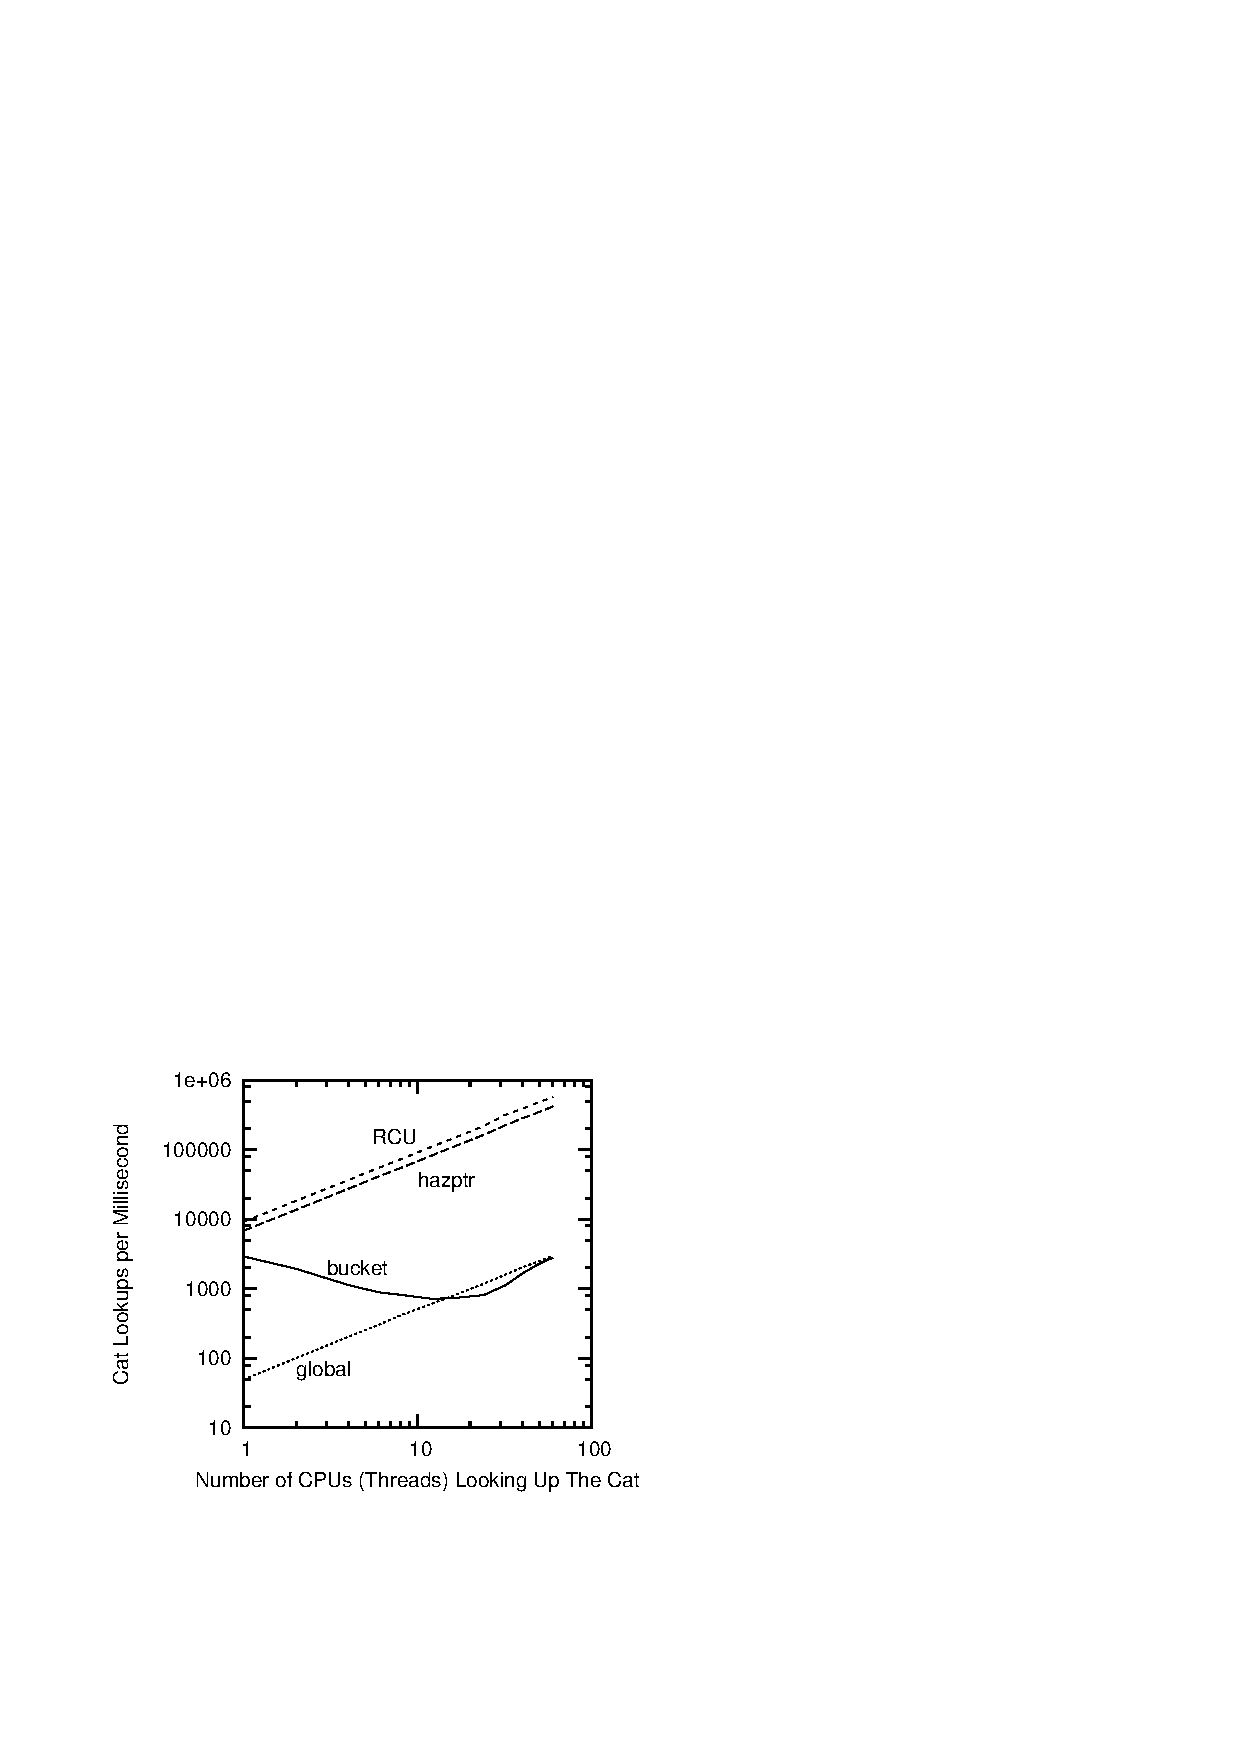
\includegraphics{datastruct/zoocatonly}}
\caption{Read-Side Cat-Only RCU-Protected Hash-Table Performance For Schr\"odinger's Zoo at 60 CPUs}
\label{fig:datastruct:Read-Side Cat-Only RCU-Protected Hash-Table Performance For Schroedinger's Zoo at 60 CPUs}
\end{figure}

앞서 언급했듯, Schr\"odinger 는 그의 고양이의 인기에
놀랐고~\cite{ErwinSchroedinger1935Cat}, 이 인기도를 그의 설계에 반영해야 할
필요가 있음을 깨달았습니다.
Figure~\ref{fig:datastruct:Read-Side Cat-Only RCU-Protected Hash-Table Performance For Schroedinger's Zoo at 60 CPUs}
는 60-CPU 가 동작하는 상황에서 고양이를 검색하는 CPU 의 숫자를 바꿔가면서 성능
결과를 비교해 봅니다.
RCU 와 해저드 포인터 모두 이 상황에 잘 동작하지만 bucket 락킹은 오히려 성능이
떨어지는데, 결국에는 심지어 하나의 락을 사용하는 경우보다도 나쁜 결과를
보입니다.
만약 모든 CPU 가 고양이만을 검색하고 있다면 그 고양이의 bucket 에 연관된 락에
모두가 매이게 될테고 이는 하나의 락을 사용하는 것과 같으므로 그다지 놀라운 일도
아닙니다.
\iffalse

As noted earlier, Schr\"odinger is surprised by the popularity of his
cat~\cite{ErwinSchroedinger1935Cat}, but recognizes the need to reflect
this popularity in his design.
Figure~\ref{fig:datastruct:Read-Side Cat-Only RCU-Protected Hash-Table Performance For Schroedinger's Zoo at 60 CPUs}
shows the results of 60-CPU runs, varying the number of CPUs that are
doing nothing but looking up the cat.
Both RCU and hazard pointers respond well to this challenge, but
bucket locking scales negatively, eventually performing even worse
than global locking.
This should not be a surprise because if all CPUs are doing nothing
but looking up the cat, the lock corresponding to the cat's bucket
is for all intents and purposes a global lock.
\fi

이 고양이만을 위한 벤치마크는 완전히 파티셔닝된 샤딩 방법에 존재할 수 있는
잠재적 문제를 보이고 있습니다.
이 고양이의 파티션에 연관된 CPU 만이 그 고양이에 접근할 수 있게 되어서,
고양이만 검색될 때의 성능을 제한하게 됩니다.
물론, 수많은 어플리케이션이 로드 오퍼레이션을 다양하게 흩뿌리는 특성을 가지고
있고, 그런 어플리케이션들에서 샤딩 방법은 매우 잘 동작할 겁니다.
하지만, 샤딩은 ``핫 스팟'' 을 아주 잘 처리하지는 못하고, Schr\"odiger 의 고양이
예제는 그런 하나의 케이스를 보이고 있습니다.
\iffalse

This cat-only benchmark illustrates one potential problem with
fully partitioned sharding approaches.
Only the CPUs associated with the cat's
partition is able to access the cat, limiting the cat-only
throughput.
Of course, a great many applications have good load-spreading
properties, and for these applications sharding works
quite well.
However, sharding does not handle ``hot spots'' very well, with
the hot spot exemplified by Schr\"odinger's cat being but one case
in point.
\fi

\begin{figure}[tb]
\centering
\resizebox{2.5in}{!}{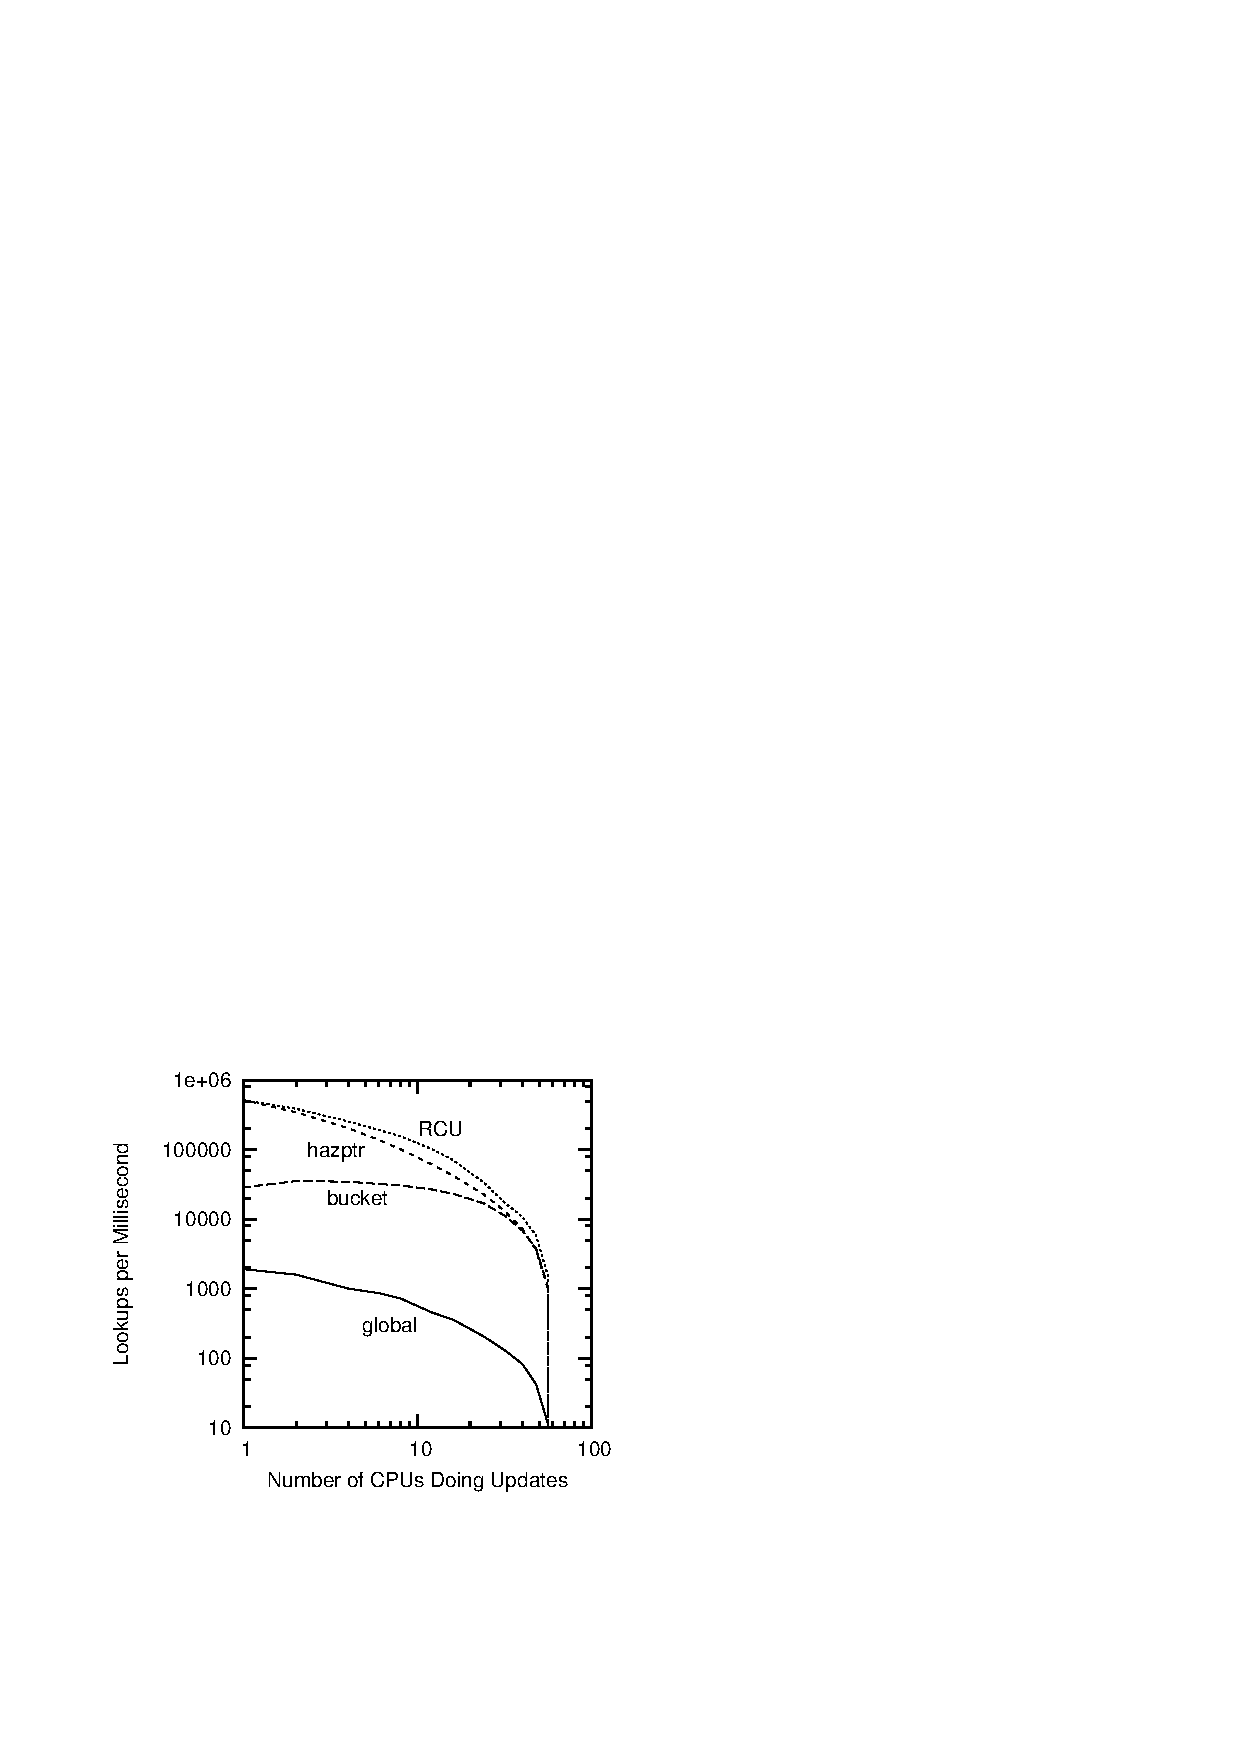
\includegraphics{datastruct/zooupdatelu}}
\caption{Read-Side RCU-Protected Hash-Table Performance For Schr\"odinger's Zoo at 60 CPUs}
\label{fig:datastruct:Read-Side RCU-Protected Hash-Table Performance For Schroedinger's Zoo at 60 CPUs}
\end{figure}

물론, 데이터를 읽기만 할 셈이라면, 애초에 동시성 제어가 필요하지도 않을 겁니다.
따라서, Figure~\ref{fig:datastruct:Read-Side RCU-Protected Hash-Table Performance For Schroedinger's Zoo at 60 CPUs}
는 업데이트의 영향을 보입니다.
이 그래프의 왼쪽 끝에서는 60 개의 모든 CPU 들이 검색만을 하고, 오른쪽 끝에서는
모든 60개의 CPU 들이 업데이트만을 합니다.
네개의 구현 모두, 밀리세컨드당 검색의 수는 업데이트를 하는 CPU 들의 수가
늘어날수록 감소되고, 60개의 모든 CPU 들이 업데이트를 하게 될 때에는
밀리세컨드당 검색의 수가 0이 되어버립니다.
RCU 는 해저드 포인터에 비해 상대적으로 좋은 결과를 보이는데 해저드 포인터의
read-side 메모리 배리어는 업데이트가 증가함에 따라 더 커다란 오버헤드를 내기
때문입니다.
따라서 최신의 하드웨어는 메모리 배리어 수행을 많이 최적화 해서 읽기만 할 때의
메모리 배리어 오버헤드를 많이 줄일 것으로 보입니다.
\iffalse

Of course, if we were only ever going to read the data, we would not need
any concurrency control to begin with.
Figure~\ref{fig:datastruct:Read-Side RCU-Protected Hash-Table Performance For Schroedinger's Zoo at 60 CPUs}
therefore shows the effect of updates.
At the extreme left-hand side of this graph, all 60 CPUs are doing lookups,
while to the right all 60 CPUs are doing updates.
For all four implementations, the number of lookups per millisecond
decreases as the number of updating CPUs increases, of course reaching
zero lookups per millisecond when all 60 CPUs are updating.
RCU does well relative to hazard pointers due to the fact that hazard
pointers's read-side memory barriers incur greater overhead in the
presence of updates.
It therefore seems likely that modern hardware heavily optimizes memory-barrier
execution, greatly reducing memory-barrier overhead in the read-only case.
\fi

\begin{figure}[tb]
\centering
\resizebox{2.5in}{!}{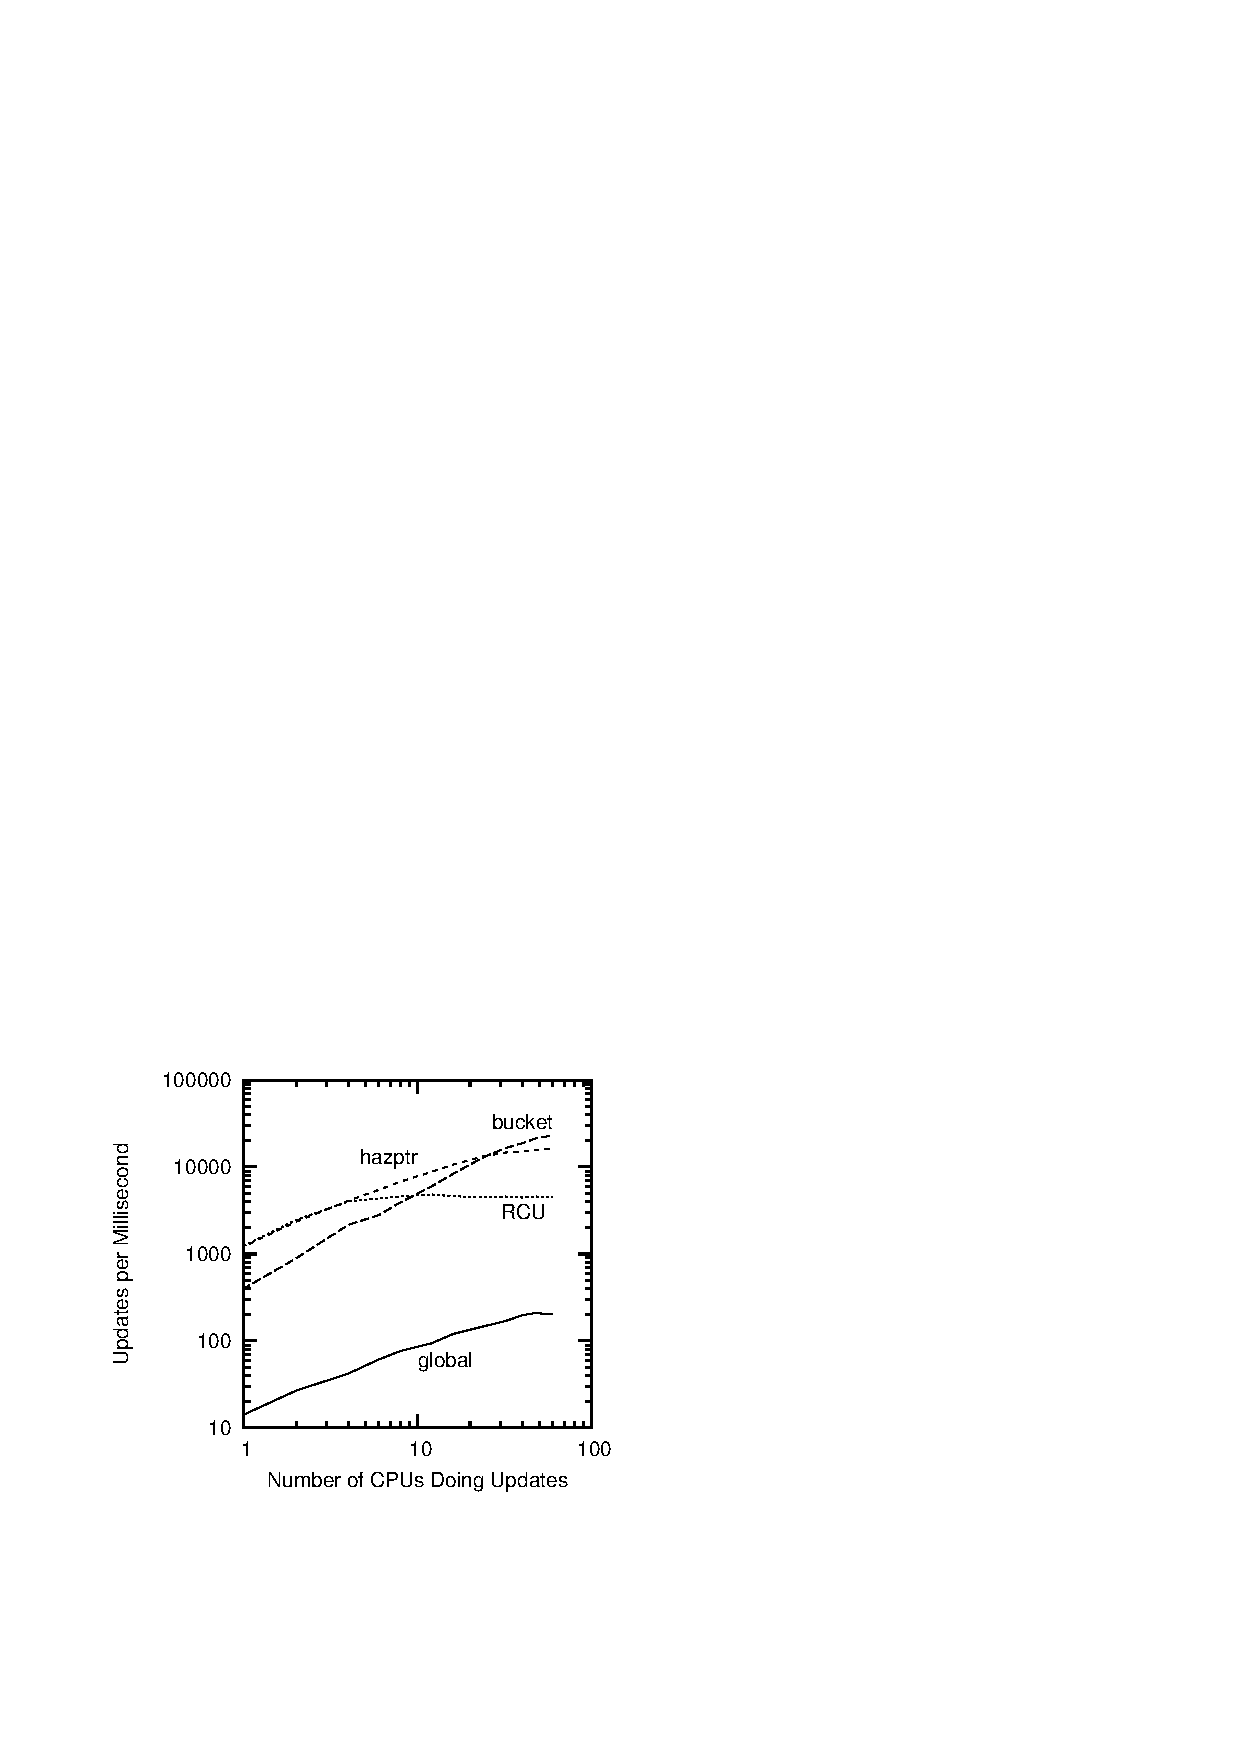
\includegraphics{datastruct/zooupdate}}
\caption{Update-Side RCU-Protected Hash-Table Performance For Schr\"odinger's Zoo at 60 CPUs}
\label{fig:datastruct:Update-Side RCU-Protected Hash-Table Performance For Schroedinger's Zoo at 60 CPUs}
\end{figure}

Figure~\ref{fig:datastruct:Read-Side RCU-Protected Hash-Table Performance For Schroedinger's Zoo at 60 CPUs}
는 검색을 하는 와중에 업데이트의 비율에 따른 영향을 보았다면,
Figure~\ref{fig:datastruct:Update-Side RCU-Protected Hash-Table Performance For Schroedinger's Zoo at 60 CPUs}
는 업데이트 자신에 대해 증가하는 업데이트 비율의 영향을 보이고 있습니다.
해저드 포인터와 RCU 는 시작점부터 상당히 좋은 성능을 가지고 시작하는데, bucket
락킹과 달리, 읽기 쓰레드들은 업데이트 쓰레드들을 막지 않기 때문입니다.
하지만, 업데이트를 하는 CPU 의 수가 늘어남에 따라, 업데이트 쪽 오버헤드는 그
존재를 드러내기 시작해서, RCU 에서 먼저 드러내고, 뒤이어 해저드 포인터에서도
보입니다.
물론, 이 세개의 구현 모두 하나의 락을 사용하는 경우에 비해서는 훨씬 좋은 성능을
보입니다.
\iffalse

Where
Figure~\ref{fig:datastruct:Read-Side RCU-Protected Hash-Table Performance For Schroedinger's Zoo at 60 CPUs}
showed the effect of increasing update rates on lookups,
Figure~\ref{fig:datastruct:Update-Side RCU-Protected Hash-Table Performance For Schroedinger's Zoo at 60 CPUs}
shows the effect of increasing update rates on the updates themselves.
Hazard pointers and RCU start off with a significant advantage because,
unlike bucket locking, readers do not exclude updaters.
However, as the number of updating CPUs increases, update-side overhead
starts to make its presence known, first for RCU and then for hazard
pointers.
Of course, all three of these implementations fare much better than does
global locking.
\fi

물론, 검색 성능에서의 차이는 업데이트 비율의 차이에 의해 영향을 받았을 가능성이
큽니다.
이를 확인할 수 있는 한가지 방법은 인공적으로 bucket 별 락킹과 해저드
포인터에서의 업데이트 비율을 RCU 에서의 그것에 맞도록 바꿔보는 것입니다.
그렇게 하는 것은 bucket 별 락킹에서의 검색 성능을 많이 끌어올리지는 못하고,
해저드 포인터와 RCU 사이의 차이를 줄이지도 못합니다.
하지만, 해저드 포인터의 읽기 쪽 메모리 배리어를 제거하는 것은 (그렇게 해서
해저드 포인터의 불안전한 구현을 만드는 것은) 해저드 포인터와 RCU 사이의 성능
차이를 거의 없애버립니다.
비록 이 불안전한 해저드 포인터 구현은 벤치마킹 목적에 따라서는 사용될 수도
있겠지만, 제품 단계에서의 사용은 결코 추천되지 못할 것입니다.
\iffalse

Of course, it is quite possible that the differences in lookup performance
are affected by the differences in update rates.
One way to check this is to artificially throttle the update rates of
per-bucket locking and hazard pointers to match that of RCU.
Doing so does not significantly improve the lookup performace of
per-bucket locking, nor does it close the gap between hazard pointers
and RCU.
However, removing hazard pointers's read-side memory barriers
(thus resulting in an unsafe implementation of hazard pointers)
does nearly close the gap between hazard pointers and RCU.
Although this unsafe hazard-pointer implementation will
usually be reliable enough for benchmarking purposes, it is absolutely
not recommended for production use.
\fi

\QuickQuiz{}
	8개 CPU 에서 60 CPU 상황을 쓰레드 수를 늘리는 것으로 시뮬레이션
	해보는건 상당히 위험함이
	Section~\ref{sec:datastruct:Hash-Table Performance} 에서
	드러났었습니다.
	하지만 60 CPU 를 가지고 더 많은 CPU 상황을 시뮬레이션 해보는건 보다
	안전할 수 있을까요?
	\iffalse

	The dangers of extrapolating from eight CPUs to 60 CPUs was
	made quite clear in
	Section~\ref{sec:datastruct:Hash-Table Performance}.
	But why should extrapolating up from 60 CPUs be any safer?
	\fi
\QuickQuizAnswer{
	그건 보다 안전하지 않고, 유용한 방법은 이 프로그램들을 더 큰 시스템에서
	돌리는 것입니다.
	하지만, 다른 테스트는 RCU read-side 기능들은 1024 쓰레드까지도 일관된
	성능과 확장성을 제공하는 것을 보였습니다.
	\iffalse

	It isn't any safer, and a useful exercise would be to run these
	programs on larger systems.
	That said, other testing has shown that RCU read-side primitives
	offer consistent performance and scalability up to at least 1024 CPUs.
	\fi
} \QuickQuizEnd

\subsection{RCU-Protected Hash Table Discussion}
\label{sec:datastruct:RCU-Protected Hash Table Discussion}

RCU 와 해저드 포인터를 사용한 구현들로부터 얻어지는 한가지 결론은 동시에
수행되는 두개의 읽기 쓰레드들은 한 고양이의 상태에 대해 서로 다른 의견을 가질
수 있다는 겁니다.
예를 들어, 한 읽기 쓰레드는 고양이가 삭제되기 직전에 그 고양이의 데이터로의
포인터를 얻어오지만, 또다른 읽기 쓰레드는 똑같은 포인터를 삭제 직후에 얻어올
수도 있습니다.
첫번째 읽기 쓰레드는 고양이가 살아있다고 믿겠지만, 두번째 읽기 쓰레드는
고양이가 죽었다고 생각할 겁니다.
\iffalse

One consequence of the RCU and hazard-pointer implementations is
that a pair of concurrent readers might disagree on the state of
the cat.
For example, one of the readers might have fetched the pointer to
the cat's data structure just before it was removed, while another
reader might have fetched this same pointer just afterwards.
The first reader would then believe that the cat was alive, while
the second reader would believe that the cat was dead.
\fi

물론, 이 상황은 Schr\"odinger 의 고양이에 맞아 떨어집니다만, 이는 양자
(quantum) 가 아닌 고양이에도 상당히 합리적인 상황임이 드러납니다.

동물이 정확히 언제 태어나고 죽었는지 판단하는건 불가능하기 때문입니다.
\iffalse

Of course, this situation is completely fitting for Schr\"odinger's
cat, but it turns out that it is quite reasonable for normal
non-quantum cats as well.

The reason for this is that it is impossible to determine exactly
when an animal is born or dies.
\fi

이를 분명히 하기 위해, 고양이의 죽음을 맥박으로 판단한다고 생각해 봅시다.
이는 죽음을 판단하기 위해선 마지막 맥박으로부터 얼마나 오래 기다려야 하는지에
대한 질문을 만듭니다.
딱 1 밀리세컨드만 기다리는건 분명 우스운 일인데, 그렇게 되면 건강하게 살아있는
고양이도 1초 동안에도 여러번 죽은 것으로 판단될 것이기 때문입니다---그리고선
부활하겠죠---.
한달을 기다리는 것도 똑같이 우스운 일일텐데, 그렇게 되면 가여운 고양이의 죽음을
냄새로도 분명히 알 수 있게 될테니까요.
\iffalse

To see this, let's suppose that we detect a cat's death by heartbeat.
This raise the question of exactly how long we should wait after the
last heartbeat before declaring death.
It is clearly ridiculous to wait only one millisecond, because then
a healthy living cat would have to be declared dead---and then
resurrected---more than once every second.
It is equally ridiculous to wait a full month, because by that time
the poor cat's death would have made itself very clearly known
via olfactory means.
\fi

\begin{figure}[tb]
\centering
\resizebox{3in}{!}{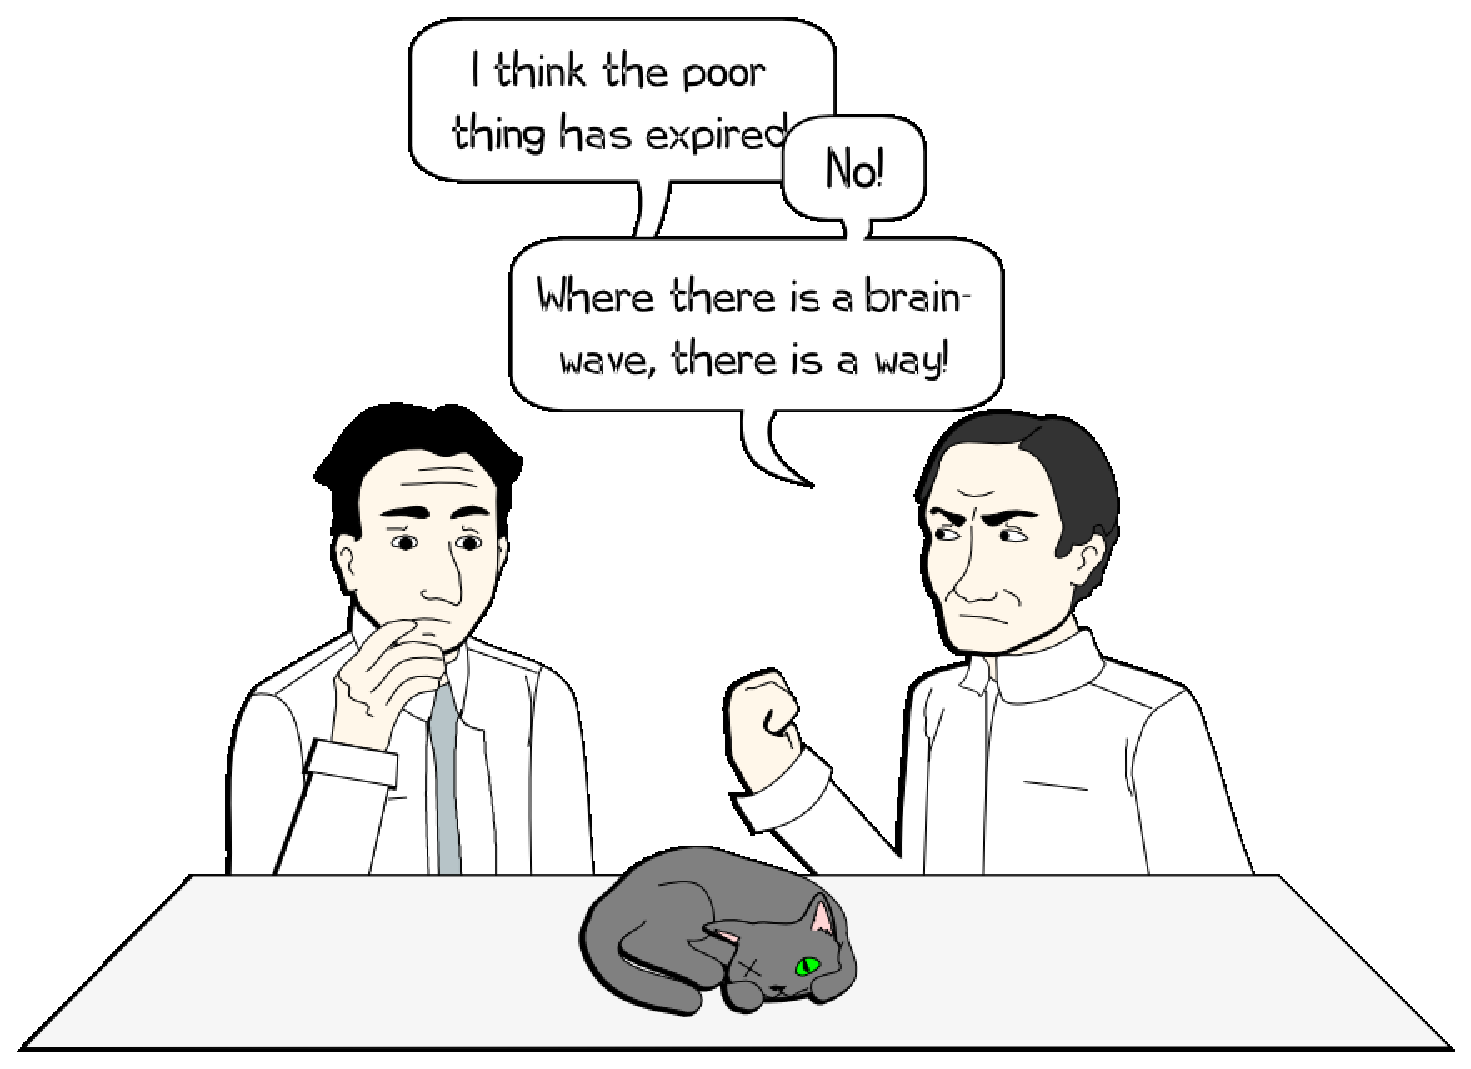
\includegraphics{cartoons/2013-08-is-it-dead}}
\caption{Even Veterinarians Disagree!}
\ContributedBy{Figure}{fig:datastruct:Even Veterinarians Disagree}{Melissa Broussard}
\end{figure}

동물의 심장은 수초동안 멈췄다가 다시 동작할 수 있으므로, 죽음의 인식과 잘못된
알람의 가능성 사이의 트레이드오프가 있습니다.
두명의 전문가도 마지막 맥박으로부터 얼마나 기다려야 죽음을 판단할 수 있는지에
대해선 의견이 갈릴 수 있습니다.
예를 들어, 한 전문가는 마지막 맥박으로부터 30초 후에 죽음을 판단할 수 있는
반면, 다른 전문가는 1분을 기다려서야 인식할 수 있습니다.
이런 경우, 두명의 전문가는
Figure~\ref{fig:datastruct:Even Veterinarians Disagree} 에 그린 것처럼 마지막
맥박으로부터 30초가 지난 후 30초 동안은 그 고양이의 상태에 대해 이견을 가질
것입니다.
\iffalse

Because an animal's heart can stop for some seconds and then start up
again, there is a tradeoff between timely recognition of death and
probability of false alarms.
It is quite possible that a pair of veterinarians might disagree on
the time to wait between the last heartbeat and the declaration of
death.
For example, one veterinarian might declare death thirty seconds after
the last heartbeat, while another might insist on waiting a full
minute.
In this case, the two veterinarians would disagree on the state of the
cat for the second period of thirty seconds following the last heartbeat,
as fancifully depicted in
Figure~\ref{fig:datastruct:Even Veterinarians Disagree}.
\fi

물론, Heisenberg 는 이런 종류의 불확실성과 함께 살아가야 한다고
가르쳤고~\cite{WeinerHeisenberg1927Uncertain}, 이는 컴퓨팅 하드웨어와
소프트웨어 역시 비슷하게 동작하기 때문에 좋은 일입니다.
예를 들어, 컴퓨팅 하드웨어의 일부 부분이 고장났는지 어떻게 아시나요?
종종 시간적으로 응답을 하지 않을때가 있죠.
고양이의 맥박처럼, 이는 하드웨어가 고장난건지 아닌지에 대한 불확실성의 기간을
만들어냅니다.
\iffalse

Of course, Heisenberg taught us to live with this sort of
uncertainty~\cite{WeinerHeisenberg1927Uncertain}, which is a good
thing because computing hardware and software acts similarly.
For example, how do you know that a piece of computing hardware
has failed?
Often because it does not respond in a timely fashion.
Just like the cat's heartbeat, this results in a window of
uncertainty as to whether or not the hardware has failed.
\fi

더 나아가서, 대부분의 컴퓨팅 시스템은 바깥 세상의 것들과 상호 동작하도록
만들어졌습니다.
따라서 이 바깥 세상의 것들과의 일관성이 무엇보다 중요합니다.
하지만,
page~\pageref{fig:defer:Response Time of RCU vs. Reader-Writer Locking} 의
Figure~\ref{fig:defer:Response Time of RCU vs. Reader-Writer Locking}
에서 봤듯이 내부의 일관성을 향상시키는 것은 외부의 일관성을 얻기 위한 비용을
증가시킬 수 있습니다.
RCU 와 해저드 포인터와 같은 테크닉들은 향상된 외부 일관성을 얻기 위해 내부
일관성을 약간 포기합니다.

요약해서, 내부의 일관성은 모든 문제 상황에서 자연적인 부분은 아니고, 종종 성능,
확장성, 외부 일관성, 그리고 그런 것들 모두의 측면에서 커다란 비용을 만듭니다.
\iffalse

Furthermore, most computing systems are intended to interact with
the outside world.
Consistency with the outside world is therefore of paramount importance.
However, as we saw in
Figure~\ref{fig:defer:Response Time of RCU vs. Reader-Writer Locking}
on
page~\pageref{fig:defer:Response Time of RCU vs. Reader-Writer Locking},
increased internal consistency can come at the expense of external
consistency.
Techniques such as RCU and hazard pointers give up some degree of
internal consistency to attain improved external consistency.

In short, internal consistency is not a natural part of all problem domains,
and often incurs great expense in terms of performance,
scalability, external consistency, or all of the above.
\fi

\section{Non-Partitionable Data Structures}
\label{sec:datastruct:Non-Partitionable Data Structures}

\begin{figure}[tb]
\centering
\resizebox{3in}{!}{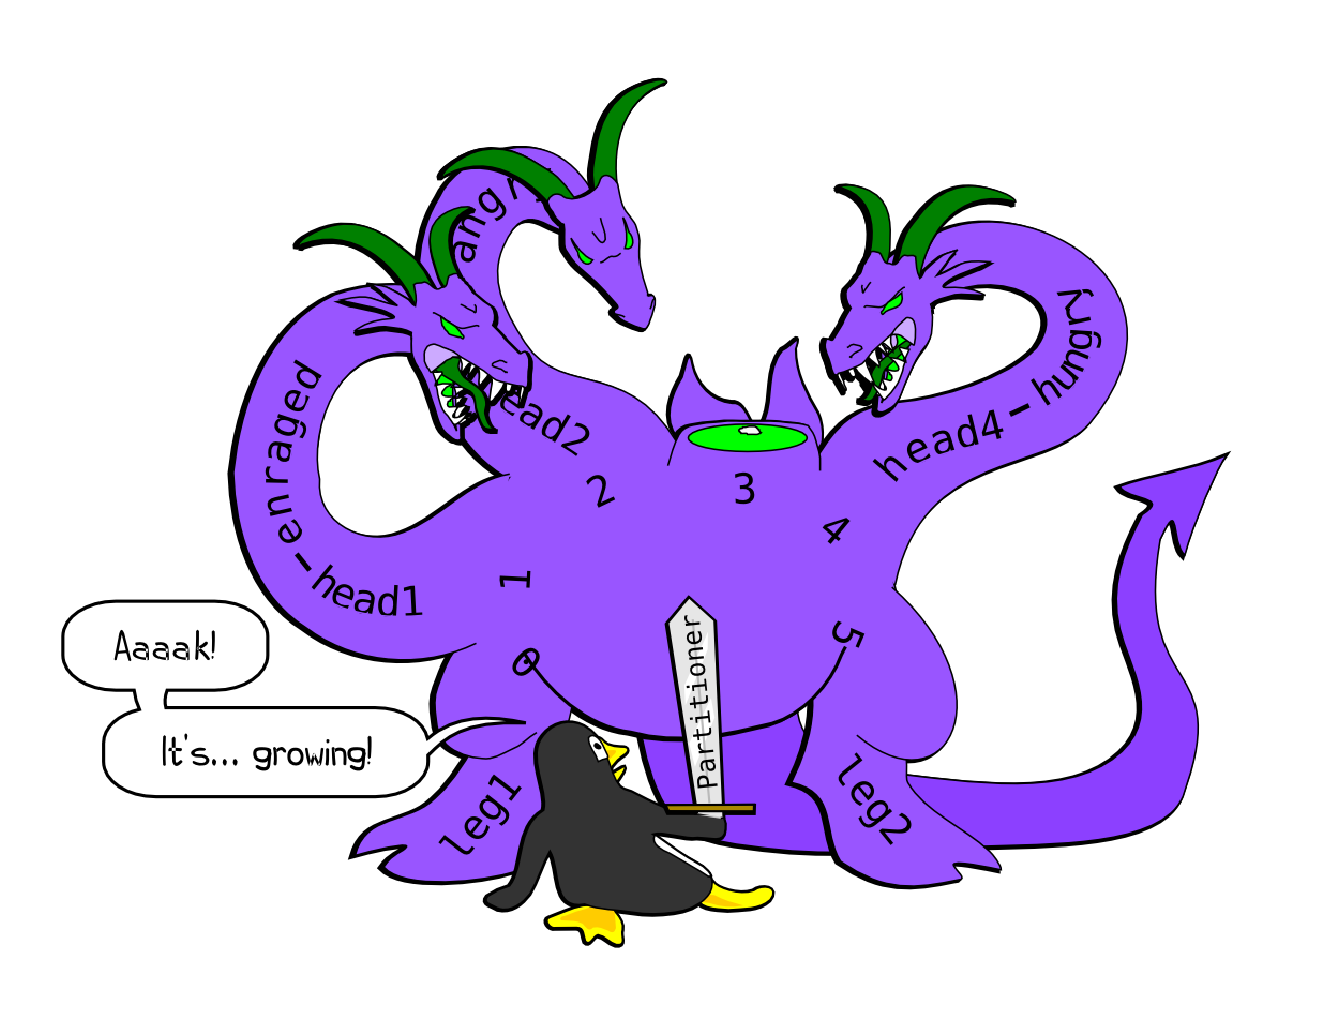
\includegraphics{cartoons/2014_Hash-table-hydra}}
\caption{Partitioning Problems}
\ContributedBy{Figure}{fig:datastruct:Partitioning Problems}{Melissa Broussard}
\end{figure}

고정크기 해시 테이블은 파티셔닝을 완전히 적용 가능하지만, 크기 조정이 가능한
해시 테이블은 크기를 키우거나 줄일 때,
Figure~\ref{fig:datastruct:Partitioning Problems} 에 보인 것처럼 파티셔닝에
있어서의 문제를 갖습니다.
하지만, 다음 섹션에서 설명하듯이 RCU 로 보호되는 고성능의 확장성 있는 해시
테이블을 만드는 것이 가능한 것으로 드러났습니다.
\iffalse

Fixed-size hash tables are perfectly partitionable, but resizable hash
tables pose partitioning challenges when growing or shrinking, as
fancifully depicted in
Figure~\ref{fig:datastruct:Partitioning Problems}.
However, it turns out that it is possible to construct high-performance
scalable RCU-protected hash tables, as described in the following sections.
\fi

\subsection{Resizable Hash Table Design}
\label{sec:datastruct:Resizable Hash Table Design}

2000년 초의 상황과 대조적으로, 이제는 다행히도 확장성 있고 RCU 로 보호되는
해시 테이블이 세개 이상의 종류가 있습니다.
첫번째의 (그리고 가장 간단한) 것은 Herbert Xu~\cite{HerbertXu2010RCUResizeHash}
에 의해 리눅스 커널을 위해 개발된 것이고, 다음 섹션에서 설명됩니다.
다른 두가지는
Section~\ref{sec:datastruct:Other Resizable Hash Tables} 에서
간단히 다루겠습니다.
\iffalse

In happy contrast to the situation in the early 2000s, there are now
no fewer than three different types of scalable RCU-protected hash
tables.
The first (and simplest) was developed for the Linux kernel by
Herbert Xu~\cite{HerbertXu2010RCUResizeHash}, and is described in the
following sections.
The other two are covered briefly in
Section~\ref{sec:datastruct:Other Resizable Hash Tables}.
\fi

첫번째 해시테이블 구현의 기저에 깔린 핵심은 각 데이터 원소가 두개의 리스트
포인터를 가질 수 있는데, 하나는 현재 RCU 읽기 쓰레드들 (과 non-RCU 업데이트
쓰레드들) 에 의해 사용되는 것이고 다른 하나는 크기가 재조정된 새로운 해시
테이블을 구성하는데 사용된다는 것입니다.
이 방법은 검색, 삽입, 그리고 삭제 작업이 크기 재조정 작업과 동시에 수행될 수
있게 합니다.
\iffalse

The key insight behind the first hash-table implementation is that
each data element can have two sets of list pointers, with one set
currently being used by RCU readers (as well as by non-RCU updaters)
and the other being used to construct a new resized hash table.
This approach allows lookups, insertions, and deletions to all run
concurrently with a resize operation (as well as with each other).
\fi

\begin{figure}[tb]
\centering
\resizebox{3in}{!}{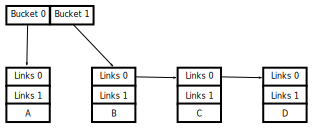
\includegraphics{datastruct/hashxu-a}}
\caption{Growing a Double-List Hash Table, State (a)}
\label{fig:datastruct:Growing a Double-List Hash Table, State (a)}
\end{figure}

\begin{figure}[tb]
\centering
\resizebox{3in}{!}{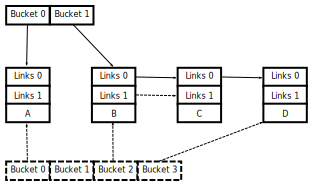
\includegraphics{datastruct/hashxu-b}}
\caption{Growing a Double-List Hash Table, State (b)}
\label{fig:datastruct:Growing a Double-List Hash Table, State (b)}
\end{figure}

크기 조정 오퍼레이션은
Figure~\ref{fig:datastruct:Growing a Double-List Hash Table, State (a)} 에 보인
최초의 두개 bucket 상태로부터 시작해서
Figures~\ref{fig:datastruct:Growing a Double-List Hash Table, State (a)}-\ref{fig:datastruct:Growing a Double-List Hash Table, State (d)}
에 보인 것처럼 진행되는데, 시간의 흐름에 따라 그림에서 그림으로 이동합니다.
최초의 상태는 원소들을 bucket 안에 연결하기 위해 zero-index 링크를 사용합니다.
네개의 새로운 bucket 배열이 할당되고, one-index 링크들이 원소들을 이 네개의
새로운 bucket 안으로 연결되는데 사용됩니다.
이는
Figure~\ref{fig:datastruct:Growing a Double-List Hash Table, State (b)} 에 보인
state~(b) 상황을 만드는데, 읽기 쓰레드들은 여전히 원래의 두개 bucket 배열을
사용하고 있습니다.
\iffalse

The resize operation proceeds as shown in
Figures~\ref{fig:datastruct:Growing a Double-List Hash Table, State (a)}-\ref{fig:datastruct:Growing a Double-List Hash Table, State (d)},
with the initial two-bucket state shown in
Figure~\ref{fig:datastruct:Growing a Double-List Hash Table, State (a)}
and with time advancing from figure to figure.
The initial state uses the zero-index links to chain the elements into
hash buckets.
A four-bucket array is allocated, and the one-index links are used to
chain the elements into these four new hash buckets.
This results in state~(b) shown in
Figure~\ref{fig:datastruct:Growing a Double-List Hash Table, State (b)},
with readers still using the original two-bucket array.
\fi

\begin{figure}[tb]
\centering
\resizebox{3in}{!}{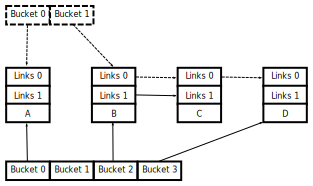
\includegraphics{datastruct/hashxu-c}}
\caption{Growing a Double-List Hash Table, State (c)}
\label{fig:datastruct:Growing a Double-List Hash Table, State (c)}
\end{figure}

\begin{figure}[tb]
\centering
\resizebox{3in}{!}{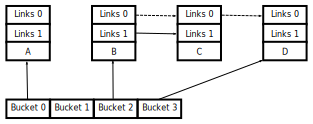
\includegraphics{datastruct/hashxu-d}}
\caption{Growing a Double-List Hash Table, State (d)}
\label{fig:datastruct:Growing a Double-List Hash Table, State (d)}
\end{figure}

새로운 네개의 bucket 배열은 읽기 쓰레드들에게 노출되고, 모든 읽기 쓰레드들을
기다리기 위해 grace-period 를 기다리게 되어서 state~(c) 에 도달하게 되는데,
Figure~\ref{fig:datastruct:Growing a Double-List Hash Table, State (c)} 에 그
상태가 그려져 있습니다.
이 상태에서, 모든 읽기 쓰레드들은 새로운 네개 bucket 배열을 사용하게 되는데, 이
말은 기존의 두개 bucket 배열은 해제되어도 좋다는 뜻이므로
Figure~\ref{fig:datastruct:Growing a Double-List Hash Table, State (d)} 에
보여진 state~(d) 로의 이전을 하게 됩니다.

이 디자인은 상대적으로 간단한 구현을 이끄는데, 이 구현에 대해서는 다음 섹션에서
다룹니다.
\iffalse

The new four-bucket array is exposed to readers and then a grace-period
operation waits for all readers, resulting in state~(c), shown in
Figure~\ref{fig:datastruct:Growing a Double-List Hash Table, State (c)}.
In this state, all readers are using the new four-bucket array,
which means that the old two-bucket array may now be freed, resulting
in state~(d), shown in
Figure~\ref{fig:datastruct:Growing a Double-List Hash Table, State (d)}.

This design leads to a relatively straightforward implementation,
which is the subject of the next section.
\fi

\subsection{Resizable Hash Table Implementation}
\label{sec:datastruct:Resizable Hash Table Implementation}

\begin{listing}[tb]
\input{CodeSamples/datastruct/hash/hash_resize@data.fcv}
\caption{Resizable Hash-Table Data Structures}
\label{lst:datastruct:Resizable Hash-Table Data Structures}
\end{listing}

\begin{lineref}[ln:datastruct:hash_resize:data]
크기 재조절은 전통적인 우회로 추가 방법으로 이루어지는데, 여기서 이 우회로는
Listing~\ref{lst:datastruct:Resizable Hash-Table Data Structures} 의 line~12-25
에 보이는 \co{ht} 구조체입니다.
Line~27-30 에 보인 \co{hashtab} 구조체는 현재의 \co{ht} 구조체로의 포인터와
해시 테이블 크기 재조정을 하려는 동시적 시도를 직렬화 하는데 사용되는
스핀락만을 담고 있습니다.
전통적인 lock 또는 어토믹 오퍼레이션 기반의 구현을 사용하려 했다면, 이
\co{hashtab} 구조체는 성능 측면에서도 확장성 측면에서도 심각한 병목지점이 될 수
있었을 겁니다.
하지만, 크기 재조정 작업은 상대적으로 가끔씩만 이뤄지므로 RCU 를 잘 사용해 볼
수 있습니다.
\iffalse

Resizing is accomplished by the classic approach of inserting a level
of indirection, in this case, the \co{ht} structure shown on
lines~\lnref{ht:b}-\lnref{ht:e} of
Listing~\ref{lst:datastruct:Resizable Hash-Table Data Structures}
(\path{hash_resize.c}).
The \co{hashtab} structure shown on
lines~\lnref{hashtab:b}-\lnref{hashtab:e} contains only a
pointer to the current \co{ht} structure along with a spinlock that
is used to serialize concurrent attempts to resize the hash table.
If we were to use a traditional lock- or atomic-operation-based
implementation, this \co{hashtab} structure could become a severe bottleneck
from both performance and scalability viewpoints.
However, because resize operations should be relatively infrequent,
we should be able to make good use of RCU.
\fi

\co{ht} 구조체는 line~13 의 \co{->ht_nbuckets} 필드를 통해 해시 테이블의 크기를
나타냅니다.
이 크기는 bucket 배열을 담고 있는 똑같은 구조체 (line~24 의 \co{->ht_bkt[]})
에도 저장되는데 이 크기와 배열 사이의 미스매치를 피하기 위해서입니다.
Line~14 에서의 \co{->ht_resize_cur} 필드는 현재 크기 재조정 작업이 진행중이지
않다면 $-1$ 이 되고, 크기 조정 작업이 진행 중이라면 line~15 의 \co{->ht_new}
필드로 레퍼런스 될, 새로운 해시 테이블에 추가될 원소의 bucket 의 인덱스를
가리키게 됩니다.
진행 중인 크기 조정 작업이 없다면, \co{->ht_new} 는 \co{NULL} 입니다.
따라서, 크기 조정 작업은 새로운 \co{ht} 구조체를 메모리 할당하고 \co{->ht_new}
포인터로 그것을 레퍼런스 한 후, \co{->ht_resize_cur} 를 기존 테이블의 bucket
들을 거쳐 증가시켜갑니다.
새로운 테이블에 모든 원소가 추가되었다면, 새로운 테이블은 \co{hashtab} 구조체의
\co{->ht_cur} 필드로 연결됩니다.
기존의 읽기 쓰레드들이 모두 완료되면, 기존의 해시 테이블의 \co{ht} 구조체는
메모리에서 해제될 수 있을 겁니다.
\iffalse

The \co{ht} structure represents a specific size of the hash table,
as specified by the \co{->ht_nbuckets} field on line~\lnref{ht:nbuckets}.
The size is stored in the same structure containing the array of
buckets (\co{->ht_bkt[]} on
line~\lnref{ht:bkt}) in order to avoid mismatches between
the size and the array.
The \co{->ht_resize_cur} field on
line~\lnref{ht:resize_cur} is equal to $-1$ unless a resize
operation
is in progress, in which case it indicates the index of the bucket whose
elements are being inserted into the new hash table, which is referenced
by the \co{->ht_new} field on line~\lnref{ht:new}.
If there is no resize operation in progress, \co{->ht_new} is \co{NULL}.
Thus, a resize operation proceeds by allocating a new \co{ht} structure
and referencing it via the \co{->ht_new} pointer, then advancing
\co{->ht_resize_cur} through the old table's buckets.
When all the elements have been added to the new table, the new
table is linked into the \co{hashtab} structure's \co{->ht_cur} field.
Once all old readers have completed, the old hash table's \co{ht} structure
may be freed.
\fi

Line~16 에 있는 \co{->ht_idx} 필드는 이 두개의 리스트 포인터들 중 이 해시
테이블을 통해 무엇이 사용되고 있는가를 알리고, line~3 의 \co{ht_elem}
구조체의 \co{->hte_next[]} 배열의 인덱스로 사용됩니다.

Line~\lnref{ht:cmp}-\lnref{ht:getkey} 의 \co{->ht_cmp()}, \co{->ht_gethash()},
그리고 \co{->ht_getkey()} 필드는 원소별 키와 해시 함수를 정의합니다.
\co{->ht_cmp()} 함수는 특정 키를 특정 원소와 비교하고, \co{ht_gethash()} 는
특정 키의 해시를 계산하며, \co{->ht_getkey()} 는 키를 감싸고 있는 데이터
원소로부터 키를 꺼낼 수 있게 합니다.

\co{ht_bucket} 구조체는 앞에서와 동일하고, \co{ht_elem} 구조체는 앞에서의
하나의 리스트 포인터와 달리 두개의 리스트 포인터의 원소 배열을 제공한다는 점만
다릅니다.
\iffalse

The \co{->ht_idx} field on
line~\lnref{ht:idx} indicates which of the two sets of
list pointers are being used by this instantiation of the hash table,
and is used to index the \co{->hte_next[]} array in the \co{ht_elem}
structure on line~\lnref{ht_elem:next}.

The \co{->ht_cmp()}, \co{->ht_gethash()}, and \co{->ht_getkey()} fields on
lines~\lnref{ht:cmp}-\lnref{ht:getkey}
collectively define the per-element key and the hash function.
The \co{->ht_cmp()} function compares a specified key with that of
the specified element,
the \co{->ht_gethash()} calculates the specified key's hash,
and \co{->ht_getkey()} extracts the key from the enclosing data
element.

The \co{ht_lock_state} shown on lines~\lnref{hls:b}-\lnref{hls:e}
is used to communicate lock state from a new \co{hashtab_lock_mod()}
to \co{hashtab_add()}, \co{hashtab_del()}, and \co{hashtab_unlock_mod()}.
This state prevents the algorithm from being redirected to the wrong
bucket during concurrent resize operations.

The \co{ht_bucket} structure is the same as before, and the
\co{ht_elem} structure differs from that of previous implementations
only in providing a two-element array of list pointer sets in place of
the prior single set of list pointers.
\fi

고정크기 해시 테이블에서의 bucket 선택은 상당히 간단합니다:
단순히 해시 값을 연관된 bucket 인덱스로 변환하면 됩니다.
반면에, 크기 조정이 진행되는 중이라면, 과거의 bucket 과 새로운 bucket 중 무엇을
선택할 지 결정해야 합니다.
만약 과거 테이블에서 선택될 수 있는 bucket 이 이미 새로운 테이블에
분산되었다면, 새로운 테이블에서의 bucket 이 선택되어야 합니다.
거꾸로, 과거 테이블에서 선택될 수 있는 bucket 이 아직 분산되지 않았다면, 그
bucket 은 과거 테이블에서 선택되어야 합니다.
\iffalse

In a fixed-sized hash table, bucket selection is quite straightforward:
Simply transform the hash value to the corresponding bucket index.
In contrast, when resizing, it is also necessary to determine which
of the old and new sets of buckets to select from.
If the bucket that would be selected from the old table has already
been distributed into the new table, then the bucket should be selected
from the new table as well as from the old table.
Conversely, if the bucket that would be selected from the old table
has not yet been distributed, then the bucket should be selected from
the old table.
\fi
\end{lineref}

\begin{listing}[tb]
\input{CodeSamples/datastruct/hash/hash_resize@get_bucket.fcv}
\caption{Resizable Hash-Table Bucket Selection}
\label{lst:datastruct:Resizable Hash-Table Bucket Selection}
\end{listing}

\begin{lineref}[ln:datastruct:hash_resize:get_bucket]
Bucket 선택 코드는
Listing~\ref{lst:datastruct:Resizable Hash-Table Bucket Selection} 의
line~\lnref{single:b}-\lnref{single:e} 에 \co{ht_get_bucket()}을, 그리고
line~\lnref{hsb:b}-\lnref{hsb:e} 에 \co{ht_search_bucket()} 을 보이고
있습니다.
\co{ht_get_bucket_single()} 함수는 특정 해시 테이블의 특정 키에 연관된 bucket
으로의 레퍼런스를 리턴하는데, 이때에는 크기 재조정을 고려하지 않습니다.
이 함수는 또한 line~\lnref{single:gethash} 의 패러미터~\co{b} 에 의해 레퍼런스
되는 위치로 키에 연관된 bucket 인덱스를 저장하고,
키에 연관된 해시 값을 line~\lnref{single:h} 의 패러미터~\co{h} (이게 \co{NULL}
이 아니라면) 에 의해 레퍼런스 되는 위치로 저장합니다.
그러고 나서 line~\lnref{single:return} 은 연관된 bucket 으로의 레퍼런스를
리턴합니다.
\iffalse

Bucket selection is shown in
Listing~\ref{lst:datastruct:Resizable Hash-Table Bucket Selection},
which shows \co{ht_get_bucket()} on
lines~\lnref{single:b}-\lnref{single:e} and \co{ht_search_bucket()} on
lines~\lnref{hsb:b}-\lnref{hsb:e}.
The \co{ht_get_bucket()} function returns a reference to the bucket
corresponding to the specified key in the specified hash table, without
making any allowances for resizing.
It also stores the bucket index corresponding to the key into the location
referenced by parameter~\co{b} on
line~\lnref{single:gethash}, and the corresponding
hash value corresponding to the key into the location
referenced by parameter~\co{h} (if non-\co{NULL}) on line~\lnref{single:h}.
Line~\lnref{single:return} then returns a reference to the corresponding bucket.
\fi

\co{ht_get_bucket()} 함수는 해시 테이블 선택을 처리하는데, line~16 에서
\co{ht_get_bucket_single()} 을 호출해서 현재 해시 테이블에서 해시 값에 연관된
bucket 을 선택하는데, 이 해시 값은 패러미터 \co{b} 에 저장됩니다.
Line~17 에서 이 테이블이 크기 재조정 중이고 line~16 의 bucket 이 이미 새로운
해시 테이블로 분산되었다는 점을 알게 되면, line~18 에서 새 해시 테이블을
선택하고 line~19 에서 이 새로운 해시 테이블에서의 해시 값에 연관된 bucket 을
선택하고, 이때에도 해시 값은 패러미터 \co{b} 에 저장합니다.
\iffalse

The \co{ht_search_bucket()} function searches for the specified key
within the specified hash-table version.
Line~\lnref{hsb:get_curbkt} obtains a reference to the bucket corresponding
to the specified key.
The loop spanning lines~\lnref{hsb:loop:b}-\lnref{hsb:loop:e} searches
that bucket, so that if line~\lnref{hsb:match} detects a match,
line~\lnref{hsb:ret_match} returns a pointer to the enclosing data element.
Otherwise, if there is no match,
line~\lnref{hsb:ret_NULL} returns \co{NULL} to indicate
failure.
\fi
\end{lineref}

\QuickQuiz{}
	Listing~\ref{lst:datastruct:Resizable Hash-Table Bucket Selection}
	의 코드는 선택된 bucket 에서 진행중일 수도 있는 크기 재조정
	프로세스로부터의 보호는 어떻게 하나요?
	\iffalse

	How does the code in
	Listing~\ref{lst:datastruct:Resizable Hash-Table Bucket Selection}
	protect against the resizing process progressing past the
	selected bucket?
	\fi
\QuickQuizAnswer{
	그런 보호는 전혀 이루어지지 않고 있습니다.
	그건 뒤에서 설명될 업데이트 쪽 동시성 제어 함수에서 할 일입니다.
	\iffalse

	It does not provide any such protection.
	That is instead the job of the update-side concurrency-control
	functions described next.
	\fi
} \QuickQuizEnd

이와 같은 \co{ht_get_bucket_single()} 와 \co{ht_get_bucket()} 의 구현은 크기
재조정 작업과 동시에 탐색과 수정이 가능하게 할 겁니다.
\iffalse

This implementation of \co{ht_get_bucket()} and \co{ht_search_bucket()}
permits lookups and modifications to run concurrently with a resize
operation.
\fi

\begin{listing}[tb]
\input{CodeSamples/datastruct/hash/hash_resize@lock_unlock_mod.fcv}
\caption{Resizable Hash-Table Update-Side Concurrency Control}
\label{lst:datastruct:Resizable Hash-Table Update-Side Concurrency Control}
\end{listing}

Read-side 동시성 제어는
Listing~\ref{lst:datastruct:RCU-Protected Hash-Table Read-Side Concurrency Control}
에서 보인 것처럼 RCU 로 제공됩니다만, update-side 동시성 제어 함수인
\co{hashtab_lock_mod()} 와 \co{hashtab_unlock_mod()} 는
Listing~\ref{lst:datastruct:Resizable Hash-Table Update-Side Concurrency Control}
에 보인 것처럼 동시적인 크기 재조정 오퍼레이션의 존재 가능성을 처리해야 합니다.
\iffalse

Read-side concurrency control is provided by RCU as was shown in
Listing~\ref{lst:datastruct:RCU-Protected Hash-Table Read-Side Concurrency Control},
but the update-side concurrency\-/control functions
\co{hashtab_lock_mod()} and \co{hashtab_unlock_mod()}
must now deal with the possibility of a
concurrent resize operation as shown in
Listing~\ref{lst:datastruct:Resizable Hash-Table Update-Side Concurrency Control}.
\fi

이 일람표의 line~1-19 에 \co{hashtab_lock_mod()} 가 있습니다.
Line~9 는 데이터 구조가 횡단을 하는 도중에 해제되는 일을 막기 위해 RCU
read-side 크리티컬 섹션에 들어가고, line~10 에서 현재 해시 테이블로의
레퍼런스를 얻어온 후, line~11 에서 이 해시 테이블에서 현재 키에 연관되는 bucket
으로의 레퍼런스를 얻어옵니다.
Line~12 는 이 bucket 의 락을 획득하는데, 이 락은 동시의 크기 재조정
오퍼레이션이 그 bucket 을 분산시키는 것을 막는데, 물론 크기 재조정 오퍼레이션이
이미 이 bucket 을 분산시켰다면 아무 영향이 없을 것임에도 불구하고 그렇습니다.
Line~13 에서는 동시의 크기 재조정 오퍼레이션이 이미 이 bucket 을 새 해시
테이블에 분산시켰는지 확인해보고, 그렇지 않다면 line~14 에서 선택된 bucket 의
락을 잡은채로 (그리고 RCU read-side 크리티컬 섹션 안에 들어와 있는 채로)
리턴합니다.
\iffalse

\begin{lineref}[ln:datastruct:hash_resize:lock_unlock_mod:l]
The \co{hashtab_lock_mod()} spans
lines~\lnref{b}-\lnref{e} in the listing.
Line~\lnref{rcu_lock} enters an RCU read-side critical section to prevent
the data structures from being freed during the traversal,
line~\lnref{refhashtbl} acquires a reference to the current hash table, and then
line~\lnref{refbucket} obtains a reference to the bucket in this hash table
corresponding to the key.
Line~\lnref{acq_bucket} acquires that bucket's lock, which will prevent any concurrent
resizing operation from distributing that bucket, though of course it
will have no effect if that bucket has already been distributed.
Lines~\lnref{lsp0b}-\lnref{lsp0e} store the bucket pointer and
pointer-set index into their respective fields in the
\co{ht_lock_state} structure, which communicates the information to
\co{hashtab_add()}, \co{hashtab_del()}, and \co{hashtab_unlock_mod()}.
Line~\lnref{ifresized} then checks to see if a concurrent resize
operation has already distributed this bucket across the new hash table,
and if not, line~\lnref{lsp1_1} indicates that there is no
already-resized hash bucket and
line~\lnref{fastret1} returns with the selected hash bucket's
lock held (thus preventing a concurrent resize operation from distributing
this bucket) and also within an RCU read-side critical section.
\fi

그렇지 않다면, 동시의 크기 재조정 오퍼레이션이 이미 이 bucket 을 분산시킨
것이므로, line~15 에서 새로운 해시 테이블로 넘어가고 line~16 에서 키에 연관되는
bucket 을 선택합니다.
마지막으로, line~17 에서 해당 bucket 의 락을 잡고 line~18 에서 기존 해시
테이블의 bucket 을 위한 락을 놓아줍니다.
다시 한번, \co{hashtab_lock_mod()} 는 RCU read-side 크리티컬 섹션 안에 들어와
있는 채로 빠져나가집니다.
\iffalse

Otherwise, a concurrent resize operation has already distributed this
bucket, so line~\lnref{new_hashtbl} proceeds to the new hash table,
line~\lnref{get_newbkt} selects the bucket corresponding to the key,
and line~\lnref{acq_newbkt} acquires the bucket's lock.
Lines~\lnref{lsp1b}-\lnref{lsp1e} store the bucket pointer and
pointer-set index into their respective fields in the 
\co{ht_lock_state} structure, which again communicates this information to
\co{hashtab_add()}, \co{hashtab_del()}, and \co{hashtab_unlock_mod()}.
Because this bucket has already been resized and because
\co{hashtab_add()} and \co{hashtab_del()} affect both the old and the
new \co{ht_bucket} structures, two locks are held, one on each of the
two buckets.
Additionally, both elements of each array in \co{ht_lock_state} structure
are used, with the \co{[0]} element pertaining to the old \co{ht_bucket}
structure and the \co{[1]} element pertaining to the new structure.
Once again, \co{hashtab_lock_mod()} exits within an RCU read-side critical
section.
\end{lineref}
\fi

\co{hashtab_unlock_mod()} 함수는 \co{hashtab_lock_mod()} 로 잡아 두었던 락을
놓아줍니다.
Line~28 에서 현재 해시 테이블을 고르고, line~29 에서 키에 연관된
bucket---당연히 이 bucket 은 새로운 해시 테이블에 속해 있을 수도 있습니다--- 의
레퍼런스를 증가시키기 위해 \co{ht_get_bucket()} 을 수행합니다.
Line~30 은 이 bucket 의 락을 놓고 마지막으로 line~31 에서 RCU read-side
크리티컬 섹션을 빠져나갑니다.
\iffalse

\begin{lineref}[ln:datastruct:hash_resize:lock_unlock_mod:ul]
The \co{hashtab_unlock_mod()} function releases the lock(s) acquired by
\co{hashtab_lock_mod()}.
Line~\lnref{relbkt0} releases the lock on the old \co{ht_bucket} structure.
In the unlikely event that line~\lnref{ifbkt1} determines that a resize
operation is in progress, line~\lnref{relbkt1} releases the lock on the
new \co{ht_bucket} structure.
Either way, line~\lnref{rcu_unlock} exits the RCU read-side critical
section.
\end{lineref}
\fi

\QuickQuiz{}
	크기 재조정 작업이 이루어지는 사이에 한 쓰레드가 새로운 해시 테이블에
	원소를 넣는다고 생각해 봅시다.
	뒤따르는 크기 재조정 작업이 이 삽입 작업 전에 완료됨으로 인해 이 삽입
	작업이 없던 것처럼 되어버리는 문제는 어떻게 방지되고 있나요?
	\iffalse

	Suppose that one thread is inserting an element into the
	hash table during a resize operation.
	What prevents this insertion from being lost due to a subsequent
	resize operation completing before the insertion does?
	\fi
\QuickQuizAnswer{
	두번째 크기 재조정 작업은 해당 bucket 에서 삽입 작업이 이루어지고 있는
	장소로 움직일 수 없을텐데, 삽입 작업이 새로운 해시 테이블 (이 예에서의
	세개의 해시 테이블 중 두번째)의 bucket 중 하나의 락을 잡고 있기
	때문입니다.
	더 나아가서, 이 삽입 작업은 RCU read-side 크리티컬 섹션 안에 위치하고
	있습니다.
	\co{hashtab_resize()} 함수에서 봤듯이, 이 말은 첫번째 크기 재조정
	작업이 삽입의 read-side 크리티컬 섹션이 완료되기를
	\co{synchronize_rcu()} 를 이용해 기다리고 있을 것을 의미합니다.
	\iffalse

	The second resize operation will not be able to move beyond
	the bucket into which the insertion is taking place due to
	the insertion holding the lock(s) on one or both of the hash
	buckets in the hash tables.
	Furthermore, the insertion operation takes place within an
	RCU read-side critical section.
	As we will see when we examine the \co{hashtab_resize()}
	function, this means that each resize operation uses
	\co{synchronize_rcu()} invocations to wait for the insertion's
	read-side critical section to complete.
	\fi
} \QuickQuizEnd

\begin{listing}[tb]
\input{CodeSamples/datastruct/hash/hash_resize@access.fcv}
\caption{Resizable Hash-Table Access Functions}
\label{lst:datastruct:Resizable Hash-Table Access Functions}
\end{listing}

이제 bucket 선택과 동시성 제어를 다뤘으니, 이 크기 재조정 가능한 해시 테이블의
탐색과 업데이트를 할 준비가 되었습니다.
\co{hashtab_lookup()}, \co{hashtab_add()}, 그리고 \co{hashtab_del()} 함수들이
Listing~\ref{lst:datastruct:Resizable Hash-Table Access Functions} 에 보여져
있습니다.
\iffalse

Now that we have bucket selection and concurrency control in place,
we are ready to search and update our resizable hash table.
The \co{hashtab_lookup()}, \co{hashtab_add()}, and \co{hashtab_del()}
functions are shown in
Listing~\ref{lst:datastruct:Resizable Hash-Table Access Functions}.
\fi

이 그림의 line~1-21 의 \co{hashtab_lookup()} 함수는 탐색을 합니다.
Line~11 에서는 현재 해시 테이블을 가져오고 line~12 에서 특정 키에 연관된 bucket
으로의 레퍼런스를 얻어옵니다.
이 bucket 은 크기 재조정 오퍼레이션이 원하는 데이터 원소를 담고 있는 예전 해시
테이블의 bucket 에서 진행되었을 때에는 새로운 크기 재조정된 해시 테이블에
위치해 있을 겁니다.
Line~12 는 또한 각 원소의 포인터 쌍들 중 올바른 것을 고르기 위한 인덱스 역시
리턴한다는 점을 알아 두세요.
Line~13-19 의 루프는 bucket 내부를 탐색하는데, line~16 에서는 매치되는지를
판단하고, line~18 에서 데이터 원소로의 포인터를 리턴하는데, 매치되지 않는다면
line~20 에서 실패를 알리는 \co{NULL} 을 리턴합니다.
\iffalse

\begin{lineref}[ln:datastruct:hash_resize:access:lkp]
The \co{hashtab_lookup()} function on
lines~\lnref{b}-\lnref{e} of the listing does
hash lookups.
Line~\lnref{get_curtbl} fetches the current hash table and
line~\lnref{get_curbkt} searches the bucket corresponding to the
specified key.
Line~\lnref{ret} returns a pointer to the searched-for element
or \co{NULL} when the search fails.
\end{lineref}
\fi

\QuickQuiz{}
	The \co{hashtab_lookup()} function in
	Listing~\ref{lst:datastruct:Resizable Hash-Table Access Functions}
	does not account for concurrent resize operations.
	Doesn't this mean that readers might miss an element that was
	added during a resize operation?
\QuickQuizAnswer{
	No.
	As we will see soon,
	the \co{hashtab_add()} and \co{hashtab_del()} functions
	keep the old hash table up-to-date while a resize operation
	is in progress.
} \QuickQuizEnd

그림의 line~23-37 의 \co{hashtab_add()} 함수는 해시 테이블에 새로운 데이터
원소를 넣습니다.
Line~32-34 는 앞에서와 같이 키에 연관되는 bucket 으로의 포인터 (그리고 인덱스)
를 얻어오고, line~35 는 새로운 원소를 테이블에 집어넣습니다.
호출자는 동시성을 잘 제어할 것이 요구되는데, 예를 들어 \co{hashtab_add()} 호출
전에 \co{hashtab_lock_mod()} 를 호출하고, 후에 \co{hashtab_unlock_mod()} 를
호출해야 하는 것 등입니다.
이런 두개의 동시성 제어 함수들은 동시의 크기 재조정 작업들과 올바르게 순서를
맞출 겁니다: 만약 이 크기 재조정 작업이 이 데이터 원소가 넣어질 bucket 에
대해서 이미 진행되었다면, 이 원소는 새로운 테이블에 추가될 겁니다.
\iffalse

\begin{lineref}[ln:datastruct:hash_resize:access:add]
The \co{hashtab_add()} function on lines~\lnref{b}-\lnref{e} of the listing adds
new data elements to the hash table.
Line~\lnref{htbp} picks up the current \co{ht_bucket} structure into which the
new element is to be added, and line~\lnref{i} picks up the index of
the pointer pair.
Line~\lnref{add} adds the new element to the current hash bucket.
If line~\lnref{ifnew} determines that this bucket has been distributed
to a new version of the hash table, then line~\lnref{addnew} also adds the
new element to the corresponding new bucket.
The caller is required to handle concurrency, for example, by invoking
\co{hashtab_lock_mod()} before the call to \co{hashtab_add()} and invoking
\co{hashtab_unlock_mod()} afterwards.
\end{lineref}
\fi

그림의 line~39-52 의 \co{hashtab_del()} 함수는 해시 테이블에서 존재하는 원소를
하나 제거합니다.
Line~48-50 에서는 앞에서와 같이 bucket 과 인덱스를 제공하고, line~51 에서 특정
원소를 제거합니다.
\co{hashtab_add()} 에서와 같이, 호출자는 동시성 제어를 할 책임을 갖게 되고 이
동시성 제어는 동시의 크기 재조정 작업과의 동기화를 처리합니다.
\iffalse

\begin{lineref}[ln:datastruct:hash_resize:access:del]
The \co{hashtab_del()} function on
lines~\lnref{b}-\lnref{e} of the listing removes
an existing element from the hash table.
Line~\lnref{i} picks up the index of the pointer pair
and line~\lnref{del} removes the specified element from the current table.
If line~\lnref{ifnew} determines that this bucket has been distributed
to a new version of the hash table, then line~\lnref{delnew} also removes
the specified element from the corresponding new bucket.
As with \co{hashtab_add()}, the caller is responsible for concurrency
control and this concurrency control suffices for synchronizing with
a concurrent resize operation.
\end{lineref}
\fi

\QuickQuiz{}
	The \co{hashtab_add()} and \co{hashtab_del()} functions in
	Listing~\ref{lst:datastruct:Resizable Hash-Table Access Functions}
	can update two hash buckets while a resize operation is progressing.
	This might cause a poor performance if the frequency of resize operation
	is not negligible.
	Isn't it possible to reduce the cost of updates in such cases?
\QuickQuizAnswer{
	Yes, at least assuming that a slight increase in the cost of
	\co{hashtab_lookup()} is acceptable.
	One approach is shown in
	Listings~\ref{lst:datastruct:Resizable Hash-Table Access Functions (Fewer Updates)}
	and~\ref{lst:datastruct:Resizable Hash-Table Update-Side Locking Function (Fewer Updates)}
	(\path{hash_resize_s.c}).

\begin{listing}[tbh]
\input{CodeSamples/datastruct/hash/hash_resize_s@access.fcv}
\caption{Resizable Hash-Table Access Functions (Fewer Updates)}
\label{lst:datastruct:Resizable Hash-Table Access Functions (Fewer Updates)}
\end{listing}

\begin{listing}[tbh]
\input{CodeSamples/datastruct/hash/hash_resize_s@lock_mod.fcv}
\caption{Resizable Hash-Table Update-Side Locking Function (Fewer Updates)}
\label{lst:datastruct:Resizable Hash-Table Update-Side Locking Function (Fewer Updates)}
\end{listing}

	This version of \co{hashtab_add()} adds an element to
	either the old bucket if it is not resized yet, or to the new
	bucket if it has been resized, and \co{hashtab_del()} removes
	the specified element from any buckets into which it has been inserted.
	The \co{hashtab_lookup()} function searches the new bucket
	if the search of the old bucket fails, which has the disadvantage
	of adding overhead to the lookup fastpath.
	The alternative \co{hashtab_lock_mod()} returns the locking
	state of the new bucket in \co{->hbp[0]} and \co{->hls_idx[0]}
	if resize operation is in progress, instead of the perhaps
	more natural choice of \co{->hbp[1]} and \co{->hls_idx[1]}.
	However, this less-natural choice has the advantage of simplifying
	\co{hashtab_add()}.

	Further analysis of the code is left as an exercise for the reader.
} \QuickQuizEnd

\begin{listing*}[tb]
\input{CodeSamples/datastruct/hash/hash_resize@resize.fcv}
\caption{Resizable Hash-Table Resizing}
\label{lst:datastruct:Resizable Hash-Table Resizing}
\end{listing*}

실제로 자신의 크기를 재조정 하는 일은 \co{hashtab_resize} 로 수행되는데,
page~\pageref{lst:datastruct:Resizable Hash-Table Resizing} 의
Listing~\ref{lst:datastruct:Resizable Hash-Table Resizing} 에 보여져 있습니다.
Line~17 은 가장 높은 레벨의 \co{->ht_lock} 을 조건적으로 얻어오는데, 만약 락을
잡는데 실패했다면 line~18 에서 크기 재조정이 이미 진행중임을 알리기 위해
\co{-EBUSY} 를 리턴합니다.
그렇지 않다면, line~19 에서 현재 해시 테이블로의 레퍼런스를 가져오고,
line~20-24 에서 원하는 크기의 새로운 해시 테이블을 할당받습니다.
새로운 hash/key 함수들이 명시된다면, 이것들이 새로운 테이블을 위해 사용되고,
그렇지 않다면 기존 테이블의 것들을 사용합니다.
Line~25 에서 메모리 할당 실패를 확인하게 된다면 line~26 에서 \co{->ht_lock} 을
놓고 line~27 에서 실패했음을 알리는 값을 반환합니다.
\iffalse

\begin{lineref}[ln:datastruct:hash_resize:resize]
The actual resizing itself is carried out by \co{hashtab_resize}, shown in
Listing~\ref{lst:datastruct:Resizable Hash-Table Resizing} on
page~\pageref{lst:datastruct:Resizable Hash-Table Resizing}.
Line~\lnref{trylock} conditionally acquires the top-level \co{->ht_lock}, and if
this acquisition fails, line~\lnref{ret_busy} returns \co{-EBUSY} to indicate that
a resize is already in progress.
Otherwise, line~\lnref{get_curtbl} picks up a reference to the current hash table,
and lines~\lnref{alloc:b}-\lnref{alloc:e} allocate a new hash table of the desired size.
If a new set of hash/key functions have been specified, these are
used for the new table, otherwise those of the old table are preserved.
If line~\lnref{chk_nomem} detects memory-allocation failure,
line~\lnref{rel_nomem} releases \co{->ht_lock}
and line~\lnref{ret_nomem} returns a failure indication.
\fi

Line~29 는 bucket 분산 프로세스를 새로운 해시테이블로의 레퍼런스를 기존
테이블의 \co{->ht_new} 에 넣음으로써 시작합니다.
Line~30 에서는 새로운 테이블의 존재를 알지 못하는 모든 읽기 쓰레드들이 크기
재조정 작업이 진행되기 전에 완료될 것을 보장합니다.
Line~31 에서는 현재 테이블의 인덱스를 얻어오고 그 역을 새로운 해시 테이블에
저장함으로써 두개의 해시 테이블이 서로의 링크드 리스트를 덮어쓰는 것을 막는
것을 보장합니다.
\iffalse

Line~\lnref{get_curidx} picks up the current table's index and
line~\lnref{put_curidx} stores its inverse to
the new hash table, thus ensuring that the two hash tables avoid overwriting
each other's linked lists.
Line~\lnref{set_newtbl} then starts the bucket-distribution process by
installing a reference to the new table into the \co{->ht_new} field of
the old table.
Line~\lnref{sync_rcu} ensures that all readers who are not aware of the
new table complete before the resize operation continues.
\fi

Line~33-44 의 루프의 각 패스에서는 기존 해시 테이블의 bucket 의 내용물 중
하나를 새로운 해시 테이블로 옮깁니다.
Line~34 에서는 기존 테이블의 현재 bucket 으로의 레퍼런스를 가져오고, line~35
에서 해당 bucket 의 스핀락을 잡습니다.
\iffalse

Each pass through the loop spanning lines~\lnref{loop:b}-\lnref{loop:e} distributes the contents
of one of the old hash table's buckets into the new hash table.
Line~\lnref{get_oldcur} picks up a reference to the old table's current bucket
and line~\lnref{acq_oldcur} acquires that bucket's spinlock.
\end{lineref}
\fi

\QuickQuiz{}
	Listing~\ref{lst:datastruct:Resizable Hash-Table Access Functions} 의
	\co{hashtab_resize()} 함수에서, line~29 에서의 \co{->ht_new} 로의
	업데이트가 line~36 에서의 \co{->ht_resize_cur} 로의 업데이트 전에
	일어난 것으로 \co{hashtab_lookup()}, \co{hashtab_add()}, 그리고
	\co{hashtab_del()} 의 관점에 보일 것을 무엇이 보장하죠?
	달리 말해서, \co{hashtab_add()} 와 \co{hashtab_del()} 이 \co{->ht_new}
	로부터 로드된 NULL 포인터를 dereference 하는걸 뭐가 막는거죠?
	\iffalse

	\begin{lineref}[ln:datastruct:hash_resize:resize]
	In the \co{hashtab_resize()} function in
	Listing~\ref{lst:datastruct:Resizable Hash-Table Resizing},
	what guarantees that the update to \co{->ht_new} on line~\lnref{set_newtbl}
	will be seen as happening before the update to \co{->ht_resize_cur}
	on line~\lnref{update_resize} from the perspective of
	\co{hashtab_add()} and \co{hashtab_del()}?
	In other words, what prevents \co{hashtab_add()}
	and \co{hashtab_del()} from dereferencing
	a NULL pointer loaded from \co{->ht_new}?
	\end{lineref}
	\fi
\QuickQuizAnswer{
	Listing~\ref{lst:datastruct:Resizable Hash-Table Access Functions}
	의 line~30 에서의 \co{synchronize_rcu()} 는 전부터 존재한 RCU 읽기
	쓰레드들이 line~29 에서 새로운 해시 테이블로의 레퍼런스를 설치한 시점과
	line~36 에서 \co{->ht_resize_cur} 를 업데이트한 시점 사이에서
	완료되었을 것을 보장합니다.
	이 말은 \co{->ht_resize_cur} 의 음이 아닌 값을 본 모든 읽기 쓰레드들은
	\co{->ht_new} 할당 전에 시작되었을 수 없고, 따라서 새로운 해시
	테이블로의 레퍼런스를 볼 수 있어야 합니다.
	\iffalse

	\begin{lineref}[ln:datastruct:hash_resize:resize]
	The \co{synchronize_rcu()} on line~\lnref{sync_rcu} of
	Listing~\ref{lst:datastruct:Resizable Hash-Table Resizing}
	ensures that all pre-existing RCU readers have completed between
	the time that we install the new hash-table reference on
	line~\lnref{set_newtbl} and the time that we update \co{->ht_resize_cur} on
	line~\lnref{update_resize}.
	This means that any reader that sees a non-negative value
	of \co{->ht_resize_cur} cannot have started before the
	assignment to \co{->ht_new}, and thus must be able to see
	the reference to the new hash table.
	\fi

	그리고 이게 왜 업데이트쪽의 \co{hashtab_add()} 와 \co{hashtab_del()}
	함수가
	Listing~\ref{lst:datastruct:Resizable Hash-Table Update-Side Concurrency Control}
	의 \co{hashtab_lock_mod()} 와 \co{hashtab_unlock_mod()} 덕에 RCU
	read-side 크리티컬 섹션 안에 들어가야 하는 이유입니다.

	And this is why the update-side \co{hashtab_add()} and
	\co{hashtab_del()} functions must nevertheless be enclosed
	in RCU read-side critical sections, courtesy of
	\co{hashtab_lock_mod()} and \co{hashtab_unlock_mod()} in
	Listing~\ref{lst:datastruct:Resizable Hash-Table Update-Side Concurrency
	Control}.
	\end{lineref}
	\fi
} \QuickQuizEnd

\begin{lineref}[ln:datastruct:hash_resize:resize]
Line~37-42 의 루프의 각 패스에서는 데이터 원소 하나를 현재의 기존 테이블의
bucket 에서 연관된 새로운 테이블의 bucket 으로 옮기는데, 이 때 새로운 테이블의
bucket 의 락을 잡고 있습니다.
Line~\lnref{update_resize} 는 이 bucket 이 분산되었다는 것을, 그리고
Listing~\ref{lst:datastruct:Resizable Hash-Table Bucket Selection} 에 보인
\co{ht_get_bucket()} 의 것과 짝을 맞추는 전체 메모리 배리어에 의해 진행된다는
것을 알리기 위해 \co{->ht_resize_cur} 를 업데이트 합니다.
마지막으로, line~\lnref{rel_oldcur} 에서는 기존 테이블 bucket 의 락을 놓게
됩니다.
\iffalse

Each pass through the loop spanning
lines~\lnref{loop_list:b}-\lnref{loop_list:e} adds one data element
from the current old-table bucket to the corresponding new-table bucket,
holding the new-table bucket's lock during the add operation.
Line~\lnref{update_resize} updates
\co{->ht_resize_cur} to indicate that this bucket has been distributed.
Finally, line~\lnref{rel_oldcur} releases the old-table bucket lock.
\fi

일단 모든 기존 테이블의 bucket 들이 새로운 테이블로 분산되면 line~45 가
수행됩니다.
Line~45 는 새로 생성된 테이블을 현재의 것으로 보이게 만들고, line~46 에서는
(여전히 기존 테이블을 레퍼런스 하고 있을) 기존 읽기 쓰레드들이 완료되기를
기다립니다.
그리고 나서 line~47 에서는 크기 재조정 직렬화 락을 놓고, line~48 에서 기존 hash
table 을 해제하고, line~48 에서 마침내 성공했음을 리턴합니다.
\iffalse

Execution reaches line~\lnref{rcu_assign} once all old-table buckets have been distributed
across the new table.
Line~\lnref{rcu_assign} installs the newly created table as the current one, and
line~\lnref{sync_rcu_2} waits for all old readers (who might still be referencing
the old table) to complete.
Then line~\lnref{rel_master} releases the resize-serialization lock,
line~\lnref{free} frees
the old hash table, and finally line~\lnref{ret_success} returns success.
\fi
\end{lineref}

\QuickQuiz{}
	\begin{lineref}[ln:datastruct:hash_resize:resize]
	Why is there a \co{WRITE_ONCE()} on line~\lnref{update_resize}
	in Listing~\ref{lst:datastruct:Resizable Hash-Table Resizing}?
	\end{lineref}
\QuickQuizAnswer{
	\begin{lineref}[ln:datastruct:hash_resize:lock_unlock_mod]
	Together with the \co{READ_ONCE()}
	on line~\lnref{l:ifresized} in \co{hashtab_lock_mod()}
	of Listing~\ref{lst:datastruct:Resizable Hash-Table Update-Side
	Concurrency Control},
	it tells the compiler that the non-initialization accesses
	to \co{->ht_resize_cur} must remain because reads
	from \co{->ht_resize_cur} really can race with writes,
	just not in a way to change the ``if'' conditions.
	\end{lineref}
} \QuickQuizEnd

\subsection{Resizable Hash Table Discussion}
\label{sec:datastruct:Resizable Hash Table Discussion}

\begin{figure}[tb]
\centering
\resizebox{2.7in}{!}{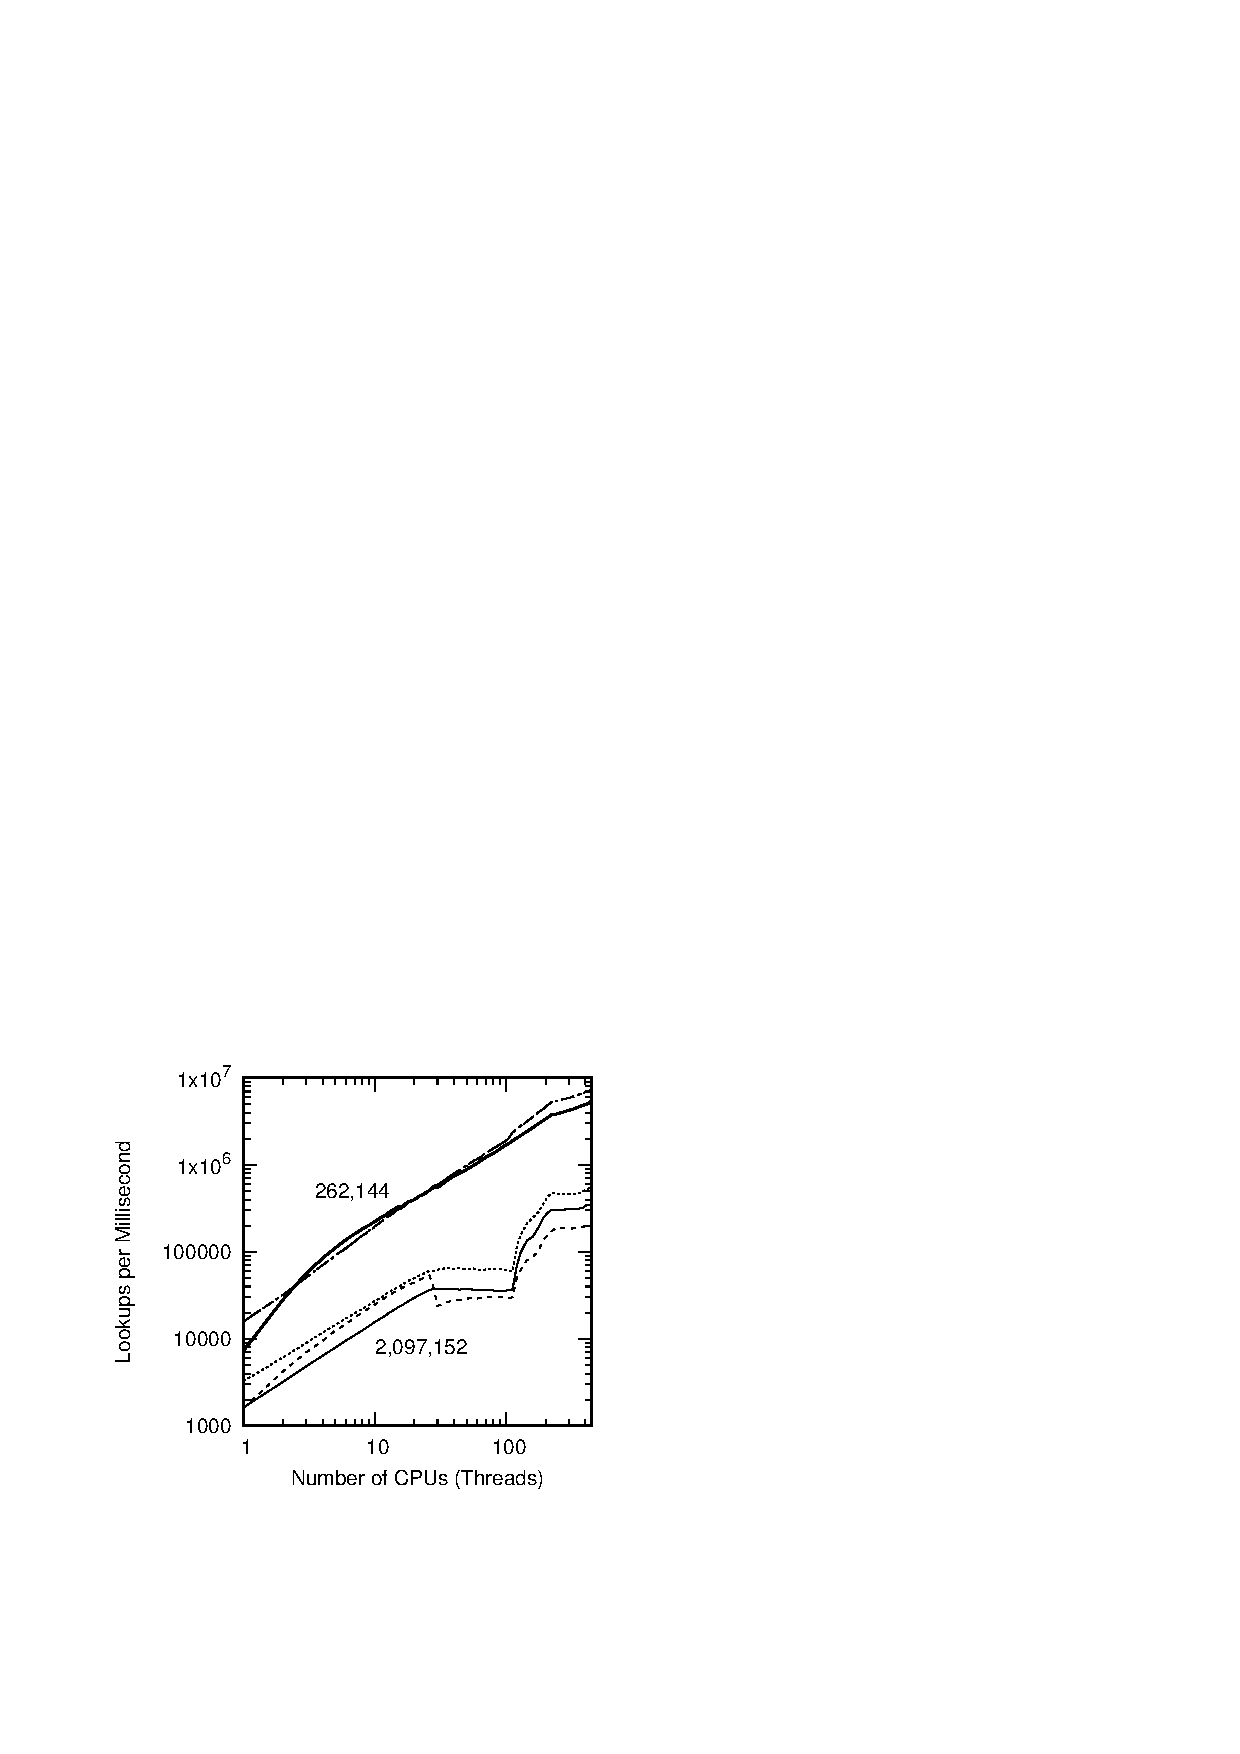
\includegraphics{datastruct/perftestresize}}
\caption{Overhead of Resizing Hash Tables}
\label{fig:datastruct:Overhead of Resizing Hash Tables}
\end{figure}

Figure~\ref{fig:datastruct:Overhead of Resizing Hash Tables}
는 크기 재조정 해시 테이블을 고정 크기 버전과 2048, 16,384, 그리고 131,702 개
원소를 가졌을 때에 대해 비교해 본 결과입니다.
이 그림은 각 원소 수마다 세개씩의 선을 보여주는데, 하나는 고정크기 1024-bucket
해시 테이블의 것이고, 하나는 고정크기 2048-bucket 해시 테이블, 나머지 하나는
1024 개와 2048 개 bucket 사이를 오갈 수 있는 크기 재조정 가능한 해시테이블
버전으로, 각각의 크기 재조정 작업 사이에는 1 밀리세컨드를 멈춥니다.
\iffalse

Figure~\ref{fig:datastruct:Overhead of Resizing Hash Tables}
compares resizing hash tables to their fixed-sized counterparts
for 2048, 16,384, and 131,072 elements in the hash table.
The figure shows three traces for each element count, one
for a fixed-size 1024-bucket hash table, another for a
fixed-size 2048-bucket hash table, and a third for a resizable
hash table that shifts back and forth between 1024 and 2048
buckets, with a one-millisecond pause between each resize operation.
\fi

가장 위의 세개의 선들은 2048 개 원소의 해시테이블의 것입니다.
위쪽 선은 2048개 bucket 을 사용하는 고정 크기 해시테이블의 것이고, 중간의 것은
1024개 bucket 을 사용하는 고정크기 해시 테이블, 그리고 아래의 것은 크기 재조정
가능한 해시 테이블입니다.
이 경우, 짧은 해시 체인들이 평범한 탐색 오버헤드를 매우 낮게 만들어서 크기
재조정 오버헤드가 지배적이게 만들었습니다.
하지만, 더 큰 고정 크기 해시 테이블이 분명한 성능 이득을 가졌으므로, 크기
재조정 작업 사이에 충분한 시간이 주어진다면 크기 재조정이 상당한 이득을 보일
겁니다: 1 밀리세컨드는 분명 너무 짧은 시간입니다.
\iffalse

The uppermost three traces are for the 2048-element hash table.
The upper trace corresponds to the 2048-bucket fixed-size hash
table, the middle trace to the 1024-bucket fixed-size hash table,
and the lower trace to the resizable hash table.
In this case, the short hash chains cause normal lookup overhead
to be so low that the overhead of resizing dominates.
Nevertheless, the larger fixed-size hash table has a significant
performance advantage, so that resizing can be quite beneficial,
at least given sufficient time between resizing operations: One
millisecond is clearly too short a time.
\fi

중간의 세개 선들은 16,384 개 원소를 가진 해시 테이블의 결과입니다.
이번에도 위쪽의 선은 2048개 bucket 을 가진 고정 크기 해시 테이블을 위한
것입니다만, 중간의 선은 크기 재조정 해시 테이블의 것이고 아래의 것은 1024개
bucket 의 고정크기 해시 테이블입니다.
하지만, 크기 재조정 버전과 1024개 bucket 버전 해시 테이블 사이의 성능 차이는
상당히 적은 것을 볼 수 있습니다.
원소의 수를 (따라서 해시 체인의 길이도) 8배로 증가시켜본 실험의 결과 중 하나는,
끊임없는 크기 재조정은 이제 너무 작은 해시 테이블을 유지하는 것보다 더 나쁘지는
않다는 것입니다.
\iffalse

The middle three traces are for the 16,384-element hash table.
Again, the upper trace corresponds to the 2048-bucket fixed-size hash
table, but the middle trace now corresponds to the resizable hash
table and the lower trace to the 1024-bucket fixed-size hash table.
However, the performance difference between the resizable and the
1024-bucket hash table is quite small.
One consequence of the eight-fold increase in number of elements
(and thus also in hash-chain length) is that incessant resizing
is now no worse than maintaining a too-small hash table.
\fi

아래쪽의 세개 선은 131,072 원소를 갖는 해시 테이블입니다.
위쪽 선은 2048 개 bucket 의 고정크기 해시 테이블이고, 중간의 것은 크기 재조정
가능 해시 테이블, 그리고 아래의 것은 1024개 bucket 사용 해시 테이블입니다.
이 경우, 더 길어진 해시체인은 높은 탐색 오버헤드를 가져왔고, 따라서 이 탐색
오버헤드가 해시 테이블의 크기 재조정을 넘어섰습니다.
하지만, 세개 해시 테이블 모두 131,072 원소 성능 수준은 2048개 원소에서의
수준보다 10배 이상 나빠졌는데, 이는 해시 테이블 크기를 64배 늘리는 것이 최고의
방법일 것임을 의미합니다.
\iffalse

The lower three traces are for the 131,072-element hash table.
The upper trace corresponds to the 2048-bucket fixed-size hash table,
the middle trace to the resizable hash table, and the lower trace
to the 1024-bucket fixed-size hash table.
In this case, longer hash chains result in higher lookup overhead,
so that this lookup overhead dominates that of resizing the hash
table.
However, the performance of all three approaches at the 131,072-element
level is more than an order of magnitude worse than that at the
2048-element level, suggesting that the best strategy would be
a single 64-fold increase in hash-table size.
\fi

이 데이터의 핵심은 RCU 로 보호되는 크기 재조정 가능한 해시 테이블은 고정 크기
버전 만큼이나 성능을 보이고 확장될 수 있다는 겁니다.
실제 크기 재조정 작업동안의 성능은 물론 안좋은데, 각 원소의 포인터들에의
업데이트가 일으키는 캐시 미스 때문일 것이고 이 영향은 해시 테이블 bucket
리스트가 짧을 때 두드러질 것입니다.
이는 해시 테이블은 상당한 크기에서 크기 재조정 되어야 하고 너무 빈번한 크기
재조정 작업으로 인한 성능 저하를 막기 위해 기록에 따른 조정(hysteresis) 을
가져야 할겁니다.
메모리가 충분히 큰 환경이라면, 해시 테이블 크기는 줄어들기보다는 더 공격적으로
증가될 수 있을 겁니다.
\iffalse

The key point from this data is that the RCU-protected resizable hash
table performs and scales almost as well as does its fixed-size counterpart.
The performance during an actual resize operation of course suffers
somewhat due to the cache misses causes by the updates to each element's
pointers, and this effect is most pronounced when the hash-tables
bucket lists are short.
This indicates that hash tables should be resized by substantial amounts,
and that hysteresis should be applied to prevent performance degradation
due to too-frequent resize operations.
In memory-rich environments, hash-table sizes should furthermore
be increased much more aggressively than they are decreased.
\fi

또다른 중요한 점은 \co{hashtab} 구조체가 분할될 수는 없지만 이것도 읽기가
대부분이므로 RCU 를 사용해 볼만 합니다.
이 크기 재조정 가능한 해시 테이블의 성능과 확장성이 RCU 로 보호되는 고정크기
해시 테이블에 근접한다는 점을 놓고 보면, 이 방법이 상당히 성공적이라고 결론내릴
수 있을 겁니다.

마지막으로, 삽입, 삭제, 그리고 탐색은 크기 재조정 작업과 동시에 이뤄질 수
있다는 점이 중요합니다.
이 동시성은 커다란 해시 테이블을 크기 재조정할 때 매우 중요한데, 특히 상당한
응답시간 제약을 가진 어플리케이션에서 그러합니다.

물론, \co{ht_elem} 구조체의 포인터 집합 쌍은 약간의 메모리 오버헤드를
내포하는데, 이에 대해서는 다음 섹션에서 이야기 합니다.
\iffalse

Another key point is that although the \co{hashtab} structure is
non-partitionable, it is also read-mostly, which suggests the use
of RCU.
Given that the performance and scalability of this resizable hash table is
very nearly that of RCU-protected fixed-sized hash tables, we must
conclude that this approach was quite successful.

Finally, it is important to note that insertions, deletions, and
lookups can proceed concurrently with a resize operation.
This concurrency is
critically important when resizing large hash tables, especially
for applications that must meet severe response-time constraints.

Of course, the \co{ht_elem} structure's
pair of pointer sets does impose some memory overhead,
which is taken up in the next section.
\fi

\subsection{Other Resizable Hash Tables}
\label{sec:datastruct:Other Resizable Hash Tables}

이 섹션의 앞에서 이야기한 크기 재조정 가능한 해시 테이블의 한계 중 하나는
메모리 사용량입니다.
각각의 데이터 원소는 한개가 아니라 두개의 링크드 리스트 포인터 쌍을 가지고
있습니다.
하나의 쌍만 가지고 일을 해낼 수 있으며 RCU 로 보호되는 크기 재조정 가능한 해시
테이블을 만들 수는 없는 걸까요?

그에 대한 답은 ``가능하다'' 로 드러났습니다.
Josh Triplett 등은 연관된 해시 체인을 점진적으로 쪼개고 조합해서 읽기
쓰레드들은 크기 재조정 작업 중간의 모든 순간에 올바른 해시 체인을 바라보게 되는
\emph{상대론적 해시 테이블}~\cite{Triplett:2011:RPHash} 을 만들었습니다.
이 점진적인 쪼개기와 조합하기는 읽기 쓰레드들이 다른 해시 체인에 있어야 하는
데이터 원소를 보게 되는 것은 문제가 되지 않는다는 사실에 기인합니다: 이런 일이
일어난다면, 읽기 쓰레드는 키가 맞지 않으므로 해당 데이터 원소를 무시해 버리게
됩니다.
\iffalse

One shortcoming of the resizable hash table described earlier in this
section is memory consumption.
Each data element has two pairs of linked-list pointers rather than just
one.
Is it possible to create an RCU-protected resizable hash table that
makes do with just one pair?

It turns out that the answer is ``yes''.
Josh Triplett et al.~\cite{Triplett:2011:RPHash}
produced a \emph{relativistic hash table} that incrementally
splits and combines corresponding hash chains so that readers always
see valid hash chains at all points during the resizing operation.
This incremental splitting and combining relies on the fact that it
is harmless for a reader to see a data element that should be in some
other hash chain: When this happens, the reader will simply ignore the
extraneous data element due to key mismatches.
\fi

\begin{figure}[tb]
\centering
\resizebox{3in}{!}{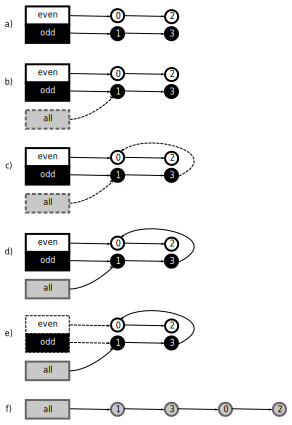
\includegraphics{datastruct/zipperhashshrink}}
\caption{Shrinking a Relativistic Hash Table}
\label{fig:datastruct:Shrinking a Relativistic Hash Table}
\end{figure}

상대론적 해시 테이블을 절반으로 축소시키는 과정이
Figure~\ref{fig:datastruct:Shrinking a Relativistic Hash Table} 에 그려져
있는데, 이 경우에는 두개의 bucket 을 가지고 있는 해시 테이블을 한개 bucket 의
해시 테이블, 달리 말해 하나의 선형 리스트로 축소시키고 있습니다.
이 과정은 기존의 커다란 해시 테이블의 한쌍의 bucket 들을 새로운 작은 해시
테이블의 하나의 bucket 으로 함치는 것으로 동작합니다.
이 프로세스가 잘 동작하려면, 두 테이블의 해시 함수에 대해 제약을 걸어야 하는
것이 분명합니다.
그런 제약 가운데 하나는 두 테이블 모두 같은 해시 함수를 사용해야 하지만, 큰
테이블에서 작은 테이블로 축소시킬 때에는 뒤쪽의 비트 하나는 버려야 한다는
것입니다.
예를 들어, 기존의 두개 bucket 을 사용하는 해시 테이블은 값의 두개의 꼭대기
비트를 사용하는 반면, 새로운 한개 bucket 의 해시 테이블은 그 값의 꼭대기 비트
하나를 사용할 겁니다.
이런 방식으로, 기존의 커다란 테이블의 인접한 짝수와 홀수 bucket 들은 새로운
작은 해시 테이블의 하나의 bucket 으로 합쳐질 수 있고, 그동안 하나의 해시 값이
이 하나의 bucket 의 원소들을 다룰 수 있습니다.
\iffalse

The process of shrinking a relativistic hash table by a factor of two
is shown in
Figure~\ref{fig:datastruct:Shrinking a Relativistic Hash Table},
in this case shrinking a two-bucket hash table into a one-bucket
hash table, otherwise known as a linear list.
This process works by coalescing pairs of buckets in the old larger hash
table into single buckets in the new smaller hash table.
For this process to work correctly, we clearly need to constrain the hash
functions for the two tables.
One such constraint is to use the same underlying hash function for
both tables, but to throw out the low-order bit when shrinking from
large to small.
For example, the old two-bucket hash table would
use the two top bits of the value, while the new one-bucket hash table
could use the top bit of the value.
In this way, a given pair of adjacent even and odd buckets in the old
large hash table can be coalesced into a single bucket in the new small
hash table, while still having a single hash value cover all of the
elements in that single bucket.
\fi

최초의 상태가 그림의 꼭대기에 보여져 있는데, 아래쪽으로 갈수록 시간이 흐르게
되고, 최초의 상황~(a) 에서 시작합니다.
축소 과정은 새로운, bucket 들의 더 작은 배열을 할당하는 것으로 시작하고, 이
새로운 작은 배열의 각각의 bucket 이 기존의 커다란 해시 테이블의 연관된 bucket
들 중 하나의 첫번째 원소를 레퍼런스 하도록 해서 상황~(b)가 되게 합니다.
\iffalse

The initial state is shown at the top of the figure, with time advancing
from top to bottom, starting with initial state~(a).
The shrinking process begins by allocating the new smaller array of
buckets, and having each bucket of this new smaller array reference
the first element of one of the buckets of the corresponding pair in
the old large hash table, resulting in state~(b).
\fi

이제 두개의 해시 체인들은 함께 연결되어서 상태~(c) 가 됩니다.
이 상태에서, 짝수로 해시값의 원소를 보는 읽기 쓰레드들은 아무 변화도 보지
못하게 되고, 원소~1 과~3 을 보는 읽기 쓰레드들은 역시 변화를 보지 못합니다.
하지만, 그와 다른 홀수 해시값의 원소를 찾는 읽기 쓰레드들은 원소~0 과~2 도
지나가게 될겁니다.
어떤 홀수 해시값도 이 두개의 원소들과 같지 않을 것이므로 이는 문제가 되지
않습니다.
이로 인한 약간의 성능 저하가 있지만, 반면에, 이는 새로운 작은 해시 테이블이
자리를 잡게 되면 겪게 될 성능 저하와 완전히 똑같은 정도입니다.
\iffalse

Then the two hash chains are linked together, resulting in state~(c).
In this state, readers looking up an even-numbered element see no change,
and readers looking up elements~1 and~3 likewise see no change.
However, readers looking up some other odd number will also traverse
elements~0 and~2.
This is harmless because any odd number will compare not-equal to these
two elements.
There is some performance loss, but on the other hand, this is exactly
the same performance loss that will be experienced once the new small
hash table is fully in place.
\fi

다음으로, 새로운 작은 해시 테이블은 읽기 쓰레드들에게 접근 가능하게 되어서
state~(d) 가 됩니다.
오래된 읽기 쓰레드들은 여전히 기존의 커다란 해시 테이블을 횡단하고 있을 수
있으므로, 이 상태는 두개의 해시 테이블을 모두 사용중인 것으로 합니다.
\iffalse

Next, the new small hash table is made accessible to readers, resulting
in state~(d).
Note that older readers might still be traversing the old large hash
table, so in this state both hash tables are in use.
\fi

다음 할 일은 모든 기존부터 존재한 읽기 쓰레드들이 완료되길 기다리는 것으로,
state~(e) 에 도달하게 됩니다.
이 상태에서, 모든 읽기 쓰레드들은 새로운 작은 해시 테이블을 사용하고 있으므로,
기존의 커다란 해시 테이블의 bucket 들은 해제될 수 있어서, 마지막 상태~(f)로
이르게 됩니다.
\iffalse

The next step is to wait for all pre-existing readers to complete,
resulting in state~(e).
In this state, all readers are using the new small hash table, so that
the old large hash table's buckets may be freed, resulting in the final
state~(f).
\fi

\begin{figure}[tb]
\centering
\resizebox{3in}{!}{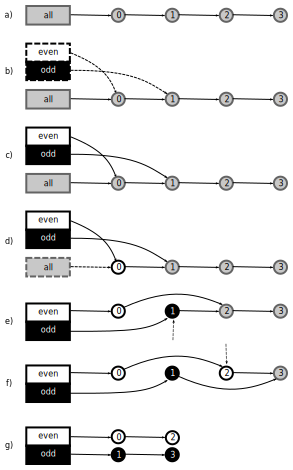
\includegraphics{datastruct/zipperhashgrow}}
\caption{Growing a Relativistic Hash Table}
\label{fig:datastruct:Growing a Relativistic Hash Table}
\end{figure}

상대론적 해시 테이블의 크기를 키우는 건 축소 프로세스의 거꾸로입니다만, 더 많은
grace-period 단계를 필요로 하게 되는데,
Figure~\ref{fig:datastruct:Growing a Relativistic Hash Table} 에 그려져
있습니다.
최소 상태~(a) 가 그림의 맨 꼭대기에 있고, 시간에 따라 아래 방향으로 진행됩니다.
\iffalse

Growing a relativistic hash table reverses the shrinking process,
but requires more grace-period steps, as shown in
Figure~\ref{fig:datastruct:Growing a Relativistic Hash Table}.
The initial state~(a) is at the top of this figure, with time advancing
from top to bottom.
\fi

새로운 커다란 두개의 bucket 을 사용하는 해시 테이블을 할당하는 것으로 시작해서,
state~(b)로 이르게 됩니다.
이 새로운 bucket들 각각은 그 bucket 을 향하게 될 첫번째 원소를 레퍼런스함을
알아두세요.
이 새로운 bucket 들은 읽기 쓰레드들에게 공개되고, 이로 인해 state~(c)로
이릅니다.
하나의 grace-period 가 지나고, 모든 읽기 쓰레드들은 새로운 커다란 해시 테이블을
사용하게 되어서 state~(d) 에 이릅니다.
이 상태에서, 짝수 해시값의 원소를 찾는 읽기 쓰레드들만이 하얀 색으로 칠해진
원소~0 을 경유하게 됩니다.
\iffalse

We start by allocating the new large two-bucket hash table, resulting
in state~(b).
Note that each of these new buckets references the first element destined
for that bucket.
These new buckets are published to readers, resulting in state~(c).
After a grace-period operation, all readers are using the new large
hash table, resulting in state~(d).
In this state, only those readers traversing the even-values hash bucket
traverse element~0, which is therefore now colored white.
\fi

이 시점에서, 기존의 작은 해시 bucket 들은 해제될 수 있지만, 많은 구현들은
아이템들의 리스트를 새로운 bucket 으로 ``풀어 놓는'' 작업의 진도 상황을 보기
위해 이 기존 bucket 들을 사용하고는 합니다.
그런 원소들의 첫번째 연속적 수행에서의 마지막 짝수 해시값 원소는 다음으로의
포인터가 다음의 짝수 해시값 원소를 가리키도록 업데이트 됩니다.
다음 grace priod 후에는, 상태~(e) 가 됩니다.
수직의 화살표는 다음으로 풀리게 될 원소를 가리키고, 원소~1 은 이제 홀수
해시값의 원소를 찾는 읽기 쓰레드들만이 다다르게 될 것을 가리키기 위해
검정색으로 칠해져 있습니다.
\iffalse

At this point, the old small hash buckets may be freed, although many
implementations use these old buckets to track progress ``unzipping''
the list of items into their respective new buckets.
The last even-numbered element in the first consecutive run of such
elements now has its pointer-to-next updated to reference the following
even-numbered element.
After a subsequent grace-period operation, the result is state~(e).
The vertical arrow indicates the next element to be unzipped, and
element~1 is now colored black to indicate that only those readers traversing
the odd-values hash bucket may reach it.
\fi

다음으로, 그런 원소들의 첫번째 연속적 수행에서의 마지막 홀수 해시값 원소가 다음
원소로의 포인터를 다음의 홀수 해시값 원소를 가리키도록 업데이트 합니다.
다음의 grace period 가 지난후, 상태~(f) 로 다다릅니다.
마지막 풀어놓기 오퍼레이션 (하나의 grace priod 를 포함해서) 은 마지막 상태~(g)
로 이르게 합니다.
\iffalse

Next, the last odd-numbered element in the first consecutive run of such
elements now has its pointer-to-next updated to reference the following
odd-numbered element.
After a subsequent grace-period operation, the result is state~(f).
A final unzipping operation (including a grace-period operation)
results in the final state~(g).
\fi

짧게 말해서, 상대론적 해시 테이블은 원소별 리스트 포인터의 수를 크기 재조정
동안 일어나는 추가적인 grace period 의 비용으로 대신합니다.
삽입, 삭제, 그리고 탐색은 크기 재조정 작업과 동시에 이루어질 수 있으므로, 이런
추가적인 grace period 들은 일반적으로 문제가 되지 않습니다.
\iffalse

In short, the relativistic hash table reduces the number of per-element
list pointers at the expense of additional grace periods incurred during
resizing.
These additional grace periods are usually not a problem because
insertions, deletions, and lookups may proceed concurrently with
a resize operation.
\fi

원소별 메모리 오버헤드가 한쌍의 포인터에서 하나의 포인터로 줄어들 수 있으면서도
여전히 $O(1)$ 삭제를 유지할 수 있음이 드러났습니다.
이는 split-order 리스트~\cite{OriShalev2006SplitOrderListHash} 를 RCU 보호로
증강시킴으로써
가능합니다~\cite{MathieuDesnoyers2009URCU,PaulMcKenney2013LWNURCUhash}.
이런 해시 테이블 안의 데이터 원소는 하나의 정렬된 링크드 리스트로 정렬되고,
각각의 해시 bucket 은 그 bucket 내의 첫번째 원소를 레퍼런스 하게 됩니다.
원소들은 다음 원소로의 포인터 필드의 아래쪽 비트를 설정하는 것으로 지워지고, 이
원소들은 그것들을 마주하게 되는 나중의 횟단에 의해 리스트에서 제거됩니다.
\iffalse

It turns out that it is possible to reduce the per-element memory overhead
from a pair of pointers to a single pointer, while still retaining
$\O{1}$ deletions.
This is accomplished by augmenting split-order
list~\cite{OriShalev2006SplitOrderListHash}
with RCU
protection~\cite{MathieuDesnoyers2009URCU,PaulMcKenney2013LWNURCUhash}.
The data elements in the hash table are arranged into a single
sorted linked list, with each hash bucket referencing the first element
in that bucket.
Elements are deleted by setting low-order bits in their pointer-to-next
fields, and these elements are removed from the list by later traversals
that encounter them.
\fi

RCU 로 보호되는 이 split-order 리스트는 복잡하지만, lock-free 진행 보장을 모든
삽입, 삭제, 그리고 탐색 작업에 제공합니다.
그런 보장사항은 리얼타임 어플리케이션들에서는 중요할 수 있습니다.
최신 버전의 userspace RCU 라이브러리~\cite{MathieuDesnoyers2009URCU} 에서 이
구현을 사용할 수 있습니다.
\iffalse

This RCU-protected split-order list is complex, but offers lock-free
progress guarantees for all insertion, deletion, and lookup operations.
Such guarantees can be important in real-time applications.
An implementation is available from recent versions of the userspace RCU
library~\cite{MathieuDesnoyers2009URCU}.
\fi

\section{Other Data Structures}
\label{sec:datastruct:Other Data Structures}

앞의 섹션들은 파티셔닝 가능성
(Section~\ref{sec:datastruct:Partitionable Data Structures}),
읽기가 대부분인 액세스 패턴의 효과적인 처리
(Section~\ref{sec:datastruct:Read-Mostly Data Structures}),
또는 읽기가 대부분인 상황에서의 테크닉을 파티셔닝이 불가능함을 해결하기 위해
적용하기
(Section~\ref{sec:datastruct:Non-Partitionable Data Structures})
로 동시성을 향상시킨 데이터 구조들에 대해 주목해 보았습니다.
이 섹션은 다른 데이터 구조들에 대해 간략한 리뷰를 합니다.
\iffalse

The preceding sections have focused on data structures that enhance
concurrency due to partitionability
(Section~\ref{sec:datastruct:Partitionable Data Structures}),
efficient handling of read-mostly access patterns
(Section~\ref{sec:datastruct:Read-Mostly Data Structures}),
or application of read-mostly techniques to avoid
non-partitionability
(Section~\ref{sec:datastruct:Non-Partitionable Data Structures}).
This section gives a brief review of other data structures.
\fi

해시 테이블의 병렬 사용에서의 가장 훌륭한 이점은 완전히 파티셔닝 가능하다는
점인데, 적어도 크기 재조정이 되지 않는 동안은 그렇습니다.
파티셔닝 가능성과 크기 독립성을 둘 다 보호하기 위한 한가지 방법은 trie 라고도
불리는 래딕스 트리(radix tree) 의 사용입니다.
Trie 들은 탐색 키를 분할하는데, 각각의 다음 키 부분을 다음 레벨의 trie 를
탐색하도록 사용하는 식입니다.
그렇게 되면, 하나의 trie 는 중첩된 해시 테이블들의 한 집합으로 생각될 수
있으므로, 필요한 파티셔닝 가능성을 제공합니다.
Trie 들의 한가지 단점은 드문드문한 키 스페이스는 메모리의 비효율적인 사용을
초래할 수 있다는 점입니다.
이런 단점을 보완할 수 있는 몇가지 압축 기법들이 존재하는데, 탐색 전에 키 값을
더 작은 키 스페이스로 해싱을 하는 방법~\cite{RobertOlsson2006a} 등이 있습니다.
래딕스 트리는 실제로 많이 사용되는데, 리눅스 커널도
포함됩니다~\cite{NickPiggin2006radixtree}.
\iffalse

One of the hash table's greatest advantages for parallel use is that it
is fully partitionable, at least while not being resized.
One way of preserving the partitionability and the size independence is
to use a radix tree, which is also called a trie.
Tries partition the search key, using each successive key partition
to traverse the next level of the trie.
As such, a trie can be thought of as a set of nested hash tables,
thus providing the required partitionability.
One disadvantage of tries is that a sparse key space can result in
inefficient use of memory.
There are a number of compression techniques that may be used to
work around this disadvantage, including hashing the key value to
a smaller keyspace before the
traversal~\cite{RobertOlsson2006a}.
Radix trees are heavily used in practice, including in the Linux
kernel~\cite{NickPiggin2006radixtree}.
\fi

해시 테이블과 trie 모두에서의 한가지 중요한 특수 케이스는 아마도 가장 오래된
데이터 구조체인 배열과 다차원 배열이라 할 수 있는, 행렬입니다.
완전히 파티셔닝 가능하다는 행렬의 본성은 동시적 수학 알고리즘에서 상당히 많이
활용되었습니다.
\iffalse

One important special case of both a hash table and a trie is what is
perhaps the oldest of data structures, the array and its multi-dimensional
counterpart, the matrix.
The fully partitionable nature of matrices is exploited heavily in
concurrent numerical algorithms.
\fi

스스로 밸런스를 잡는 트리는 순차적 코드에서 상당히 많이 사용되었는데, AVL
트리와 red-black 트리는 아마도 가장 널리 알려진 예일
겁니다~\cite{ThomasHCorman2001Algorithms}.
AVL 트리를 병렬화 하려 한 기존의 시도들은 복잡하고 그다지 효율적이지
못했습니다만~\cite{Ellis80}, 최근의 red-black 트리에서의 작업은 읽기 쓰레드에게
RCU 를 사용하고 읽기와 업데이트를 각각 보호하는데에 해시를 사용한 락들의
배열\footnote{
	개발자가 공유되지 않는 액세스를 직접 표시하는 소프트웨어 트랜잭셔널
	메모리의 하나의 변종인 swissTM~\cite{AleksandarDragovejic2011STMnotToy}
	으로 가장해서}
을 사용해서 더 나은 성능과 확장성을
제공합니다~\cite{PhilHoward2011RCUTMRBTree,PhilipWHoward2013RCUrbtree}.
Red-black 트리는 적극적으로 밸런스 재조정을 수행한다는 사실이 드러났는데, 이는
순차적 프로그램에서는 잘 동작하지만 병렬적 사용에서는 꼭 그렇지만은 않습니다.
그래서 최근의 연구는 RCU 로 보호되는 ``bonsai tree'' 를 만들어냈는데, 이 데이터
구조는 덜 적극적으로 밸런스 재조정을
해서~\cite{AustinClements2012RCULinux:mmapsem} 최적의 트리 깊이와 더 효과적인
동시의 업데이트 사이에서 트레이드 오프 합니다.
\iffalse

Self-balancing trees are heavily used in sequential code, with
AVL trees and red-black trees being perhaps the most well-known
examples~\cite{ThomasHCorman2001Algorithms}.
Early attempts to parallelize AVL trees were complex and not necessarily
all that efficient~\cite{Ellis80},
however, more recent work on red-black trees provides better
performance and scalability by using RCU for readers and hashed arrays
of locks\footnote{
	In the guise of swissTM~\cite{AleksandarDragovejic2011STMnotToy},
	which is a variant of software transactional memory in which
	the developer flags non-shared accesses.}
to protect reads and updates,
respectively~\cite{PhilHoward2011RCUTMRBTree,PhilipWHoward2013RCUrbtree}.
It turns out that red-black trees rebalance aggressively, which works
well for sequential programs, but not necessarily so well for parallel
use.
Recent work has therefore made use of RCU-protected ``bonsai trees''
that rebalance less aggressively~\cite{AustinClements2012RCULinux:mmapsem},
trading off optimal tree depth to gain more efficient concurrent updates.
\fi

동시의 스킵 리스트들 역시 RCU 읽기 쓰레드들에게 좋은데, 실제로 RCU 를 사용하는
테크닉의 사용을 초기의 학계에서 선보였습니다~\cite{Pugh90}.

동시적 double-ended 큐들은
Section~\ref{sec:SMPdesign:Double-Ended Queue} 에서 다루었고,
동시적 스택과 큐들은 긴 역사를 가지고 있습니다만~\cite{Treiber86},
일반적으로는 인상적인 성능과 확장성을 보이진 못했습니다.
하지만 이것들은 동시성 라이브러리들의 흔한 기능일
뿐입니다~\cite{PaulMcKenney2013LWNURCUqueuestack}.
연구자들은 최근에 스택과 큐의 순서 규칙을 완화시키는 것을
제안했는데~\cite{Shavit:2011:DSM:1897852.1897873}, 일부 작업은 완화된 순서
규칙의 큐가 실제로는 엄격한 FIFO 큐보다 더 나은 순서 특성을 실제로 가짐을
보이기도
했습니다~\cite{AndreasHaas2012FIFOisnt,ChristophMKirsch2012FIFOisntTR,AndreasHaas2013CFRelaxedQueues}.
\iffalse

Concurrent skip lists lend themselves well to RCU readers, and in fact
represents an early academic use of a technique resembling
RCU~\cite{Pugh90}.

Concurrent double-ended queues were discussed in
Section~\ref{sec:SMPdesign:Double-Ended Queue},
and concurrent stacks and queues have a long history~\cite{Treiber86},
though not normally the most impressive performance or scalability.
They are nevertheless a common feature of concurrent
libraries~\cite{PaulMcKenney2013LWNURCUqueuestack}.
Researchers have recently proposed relaxing the ordering constraints
of stacks and queues~\cite{Shavit:2011:DSM:1897852.1897873},
with some work indicating that relaxed-ordered queues actually have
better ordering properties than do strict FIFO
queues~\cite{AndreasHaas2012FIFOisnt,ChristophMKirsch2012FIFOisntTR,AndreasHaas2013CFRelaxedQueues}.
\fi

동시적 데이터 구조에 대한 지속적 작업은 놀라운 특성을 가진 기발한 알고리즘들을
만들어낼 것으로 보입니다.
\iffalse

It seems likely that continued work with concurrent data structures will
produce novel algorithms with surprising properties.
\fi

\section{Micro-Optimization}
\label{sec:datastruct:Micro-Optimization}

이 섹션에 보인 데이터 구조들은 간단히 코딩 되었고, 시스템 캐시 구조의 적용도
없었습니다.
또한, 구현들 중 다수가 키에서 해시로의 변환 등의 빈번한 작업들에 함수 포인터를
사용했습니다.
이런 방법은 간단하고 호환성을 높여주지만, 많은 경우에 어느정도 성능을 포기하게
합니다.

뒤의 섹션들에서는 특수화, 메모리 절약, 그리고 하드웨어 고려에 대해 다뤄봅니다.
이 짧은 섹션들이 분명한 이 주제에 대한 전문적 정리된 내용이라고 생각하는 실수를
하지 마세요.
이 내용들은 특정 CPU 에서의 최적화에 관해 쓰여진 것이므로 오늘날 흔히 사용되는
CPU 들과는 별개입니다.
\iffalse

The data structures shown in this section were coded straightforwardly,
with no adaptation to the underlying system's cache hierarchy.
In addition, many of the implementations used pointers to functions
for key-to-hash conversions and other frequent operations.
Although this approach provides simplicity and portability, in many
cases it does give up some performance.

The following sections touch on specialization, memory conservation,
and hardware considerations.
Please do not mistake these short sections for a definitive treatise
on this subject.
Whole books have been written on optimizing to a specific CPU, let
alone to the set of CPU families in common use today.
\fi

\subsection{Specialization}
\label{sec:datastruct:Specialization}

Section~\ref{sec:datastruct:Non-Partitionable Data Structures}
에 선보여진 크기 재조정 가능한 해시 테이블은 불확실한 타입의 키를 사용했습니다.
이는 높은 유연성을 가능하게 해서, 어떤 종류의 키도 사용될 수 있게 했습니다만,
또한 함수로의 포인터를 사용한 함수 호출로 인해 상당한 오버헤드를 이끌었습니다.
최신의 하드웨어는 이런 오버헤드를 최소화하기 위해 세련된 브랜치 예측 테크닉을
사용합니다만, 다른 한편으로 실제 세상의 소프트웨어는 오늘날의 커다란 하드웨어
브랜치 예측 테이블로도 수용할 수 없을만큼 큰 경우가 많습니다.
이는 특히 함수 포인터를 통한 호출의 경우에 그러한데, 이 경우에 브랜치 예측
하드웨어는 브랜치가 취해졌는지 안취해졌는지에 대한 정보에 더해서 포인터를
기록해야 하기 때문입니다.
\iffalse

The resizable hash table presented in
Section~\ref{sec:datastruct:Non-Partitionable Data Structures}
used an opaque type for the key.
This allows great flexibility, permitting any sort of key to be
used, but it also incurs significant overhead due to the calls via
of pointers to functions.
Now, modern hardware uses sophisticated branch-prediction techniques
to minimize this overhead, but on the other hand, real-world software
is often larger than can be accommodated even by today's large
hardware branch-prediction tables.
This is especially the case for calls via pointers, in which case
the branch prediction hardware must record a pointer in addition
to branch-taken/branch-not-taken information.
\fi

이 오버헤드는 해시 테이블 구현을 특정 키 타입과 해시 함수로 특수화 시킴으로써
제거될 수 있습니다.
그렇게 하는 것은
page~\pageref{lst:datastruct:Resizable Hash-Table Data Structures} 의
Listing~\ref{lst:datastruct:Resizable Hash-Table Data Structures} 에서 보인
\co{ht} 구조체에서 \co{->ht_cmp()}, \co{->ht_gethash()}, 그리고
\co{->ht_getkey()} 함수 포인터들을 제거합니다.
이는 또한 연관된 포인터들을 통한 함수 호출도 제거하는데, 이는 컴파일러가 이
고정된 함수들을 인라인 시킬 수 있게 해서 호출 명령의 오버헤드만이 아니라 인자
관리 오버헤드 역시 제거할 겁니다.
\iffalse

This overhead can be eliminated by specializing a hash-table implementation
to a given key type and hash function.
Doing so eliminates the \co{->ht_cmp()}, \co{->ht_gethash()}, and
\co{->ht_getkey()} function pointers in the \co{ht} structure shown in
Listing~\ref{lst:datastruct:Resizable Hash-Table Data Structures} on
page~\pageref{lst:datastruct:Resizable Hash-Table Data Structures}.
It also eliminates the corresponding calls through these pointers,
which could allow the compiler to inline the resulting fixed functions,
eliminating not only the overhead of the call instruction, but the
argument marshalling as well.
\fi

또한, 이 크기 재조정 가능한 해시 테이블은 동시성 제어로부터 bucket 선택을
분리하는 API 에 걸맞도록 설계되었습니다.
이는 하나의 테스트가 이 챕터의 모든 해시 테이블의 구현을 테스트할 수 있도록
해주지만, 또한 많은 연산작업들이 해시 값을 계산하고 만들어질 수 있는 크기
재조정 작업과 한번이 아니라 두번 상호작용해야 함을 의미합니다.
성능이 중요한 환경에서라면 \co{hashtab_lock_mod()} 함수 또한 선택된 bucket
으로의 레퍼런스를 리턴해서 이어지는 \co{ht_get_bucket()} 호출을 제거할
겁니다.
\iffalse

In addition, the resizable hash table is designed to fit an API
that segregates bucket selection from concurrency control.
Although this allows a single torture test to exercise all the hash-table
implementations in this chapter, it also means that many operations
must compute the hash and interact with possible resize operations twice
rather than just once.
In a performance-conscious environment, the \co{hashtab_lock_mod()}
function would also return a reference to the bucket selected, eliminating
the subsequent call to \co{ht_get_bucket()}.
\fi

\QuickQuiz{}
	\path{hashtorture.h} 의 코드는 \co{hashtab_lock_mode()} 가
	\co{ht_get_bucket()} 의 기능을 포섭하도록 수정될 수 없나요?
	\iffalse

	Couldn't the \path{hashtorture.h} code be modified to accommodate
	a version of \co{hashtab_lock_mod()} that subsumes the
	\co{ht_get_bucket()} functionality?
	\fi
\QuickQuizAnswer{
	그럴 수도 있을테고, 그렇게 하는게 이 챕터에 선보여진 bucket 별 락킹을
	사용하는 해시 테이블에 이득을 가져다 줄 수 있을 겁니다.
	이런 변경을 만드는 건 독자 여러분의 몫으로 두겠습니다.
	\iffalse

	It probably could, and doing so would benefit all of the
	per-bucket-locked hash tables presented in this chapter.
	Making this modification is left as an exercise for the
	reader.
	\fi
} \QuickQuizEnd

\QuickQuiz{}
	이런 특수화는 정말로 얼마나 성능을 구하나요?
	이게 정말 가치가 있나요?
	\iffalse

	How much do these specializations really save?
	Are they really worth it?
	\fi
\QuickQuizAnswer{
	첫번째 질문에 대한 답은 독자의 몫으로 남겨져 있습니다.
	크기 재조정 가능한 해시 테이블을 특수화 시켜보고 그 결과로 성능이
	얼마나 개선되는지 살펴보세요.
	두번째 질문은 일반적으로는 답변될 수가 없습니다만, 대신 특수한 사용
	예에 맞춰서 답변될 수 있을 겁니다.
	일부 사용 케이스는 성능과 확장성에 극단적으로 민감하고 다른 것들은
	그보다 덜할 수 있습니다.
	\iffalse

	The answer to the first question is left as an exercise to
	the reader.
	Try specializing the resizable hash table and see how much
	performance improvement results.
	The second question cannot be answered in general, but must
	instead be answered with respect to a specific use case.
	Some use cases are extremely sensitive to performance and
	scalability, while others are less so.
	\fi
} \QuickQuizEnd

그렇다고는 해도, 제가 처음 프로그램을 배우기 시작한 1970년대 초반에 사용할 수
있던 것들에 비해 최신 하드웨어의 커다란 장점중 하나는 그렇게까지나 특수화가
필요하지는 않다는 것입니다.
이는 4 킬로바이트 주소공간을 사용하던 시절에 그랬던 것에 비해 훨씬 큰 생산성을
가능하게 합니다.
\iffalse

All that aside, one of the great benefits of modern hardware compared
to that available when I first started learning to program back in
the early 1970s is that much less specialization is required.
This allows much greater productivity than was possible back in the
days of four-kilobyte address spaces.
\fi

\subsection{Bits and Bytes}
\label{sec:datastruct:Bits and Bytes}

이 챕터에서 논의한 해시 테이블들은 메모리 절약을 위한 시도는 거의 하지 않고
만들어졌습니다.
예를 들어,
page~\pageref{lst:datastruct:Resizable Hash-Table Data Structures} 의
Listing~\ref{lst:datastruct:Resizable Hash-Table Data Structures} 에 있는
\co{ht} 구조체의 \co{->ht_idx} 필드는 항상 0 또는 1 의 값을 갖는데도 32비트의
메모리를 모두 가집니다.
이건 예를 들어 \co{->ht_resize_key} 필드에서 비트 하나를 훔쳐다 사용하는 식으로
제거될 수 있을 겁니다.
이 방법은 \co{->ht_resize_key} 필드가 메모리의 모든 바이트를 가리킬 수 있을
만큼 커다랗고 \co{ht_bucket} 구조체는 1 바이트보다 크기 때문에
\co{->ht_resize_key} 필드는 몇 비트는 아낄 수 있을 것이기 때문에 동작
가능합니다.
\iffalse

The hash tables discussed in this chapter made almost no attempt to conserve
memory.
For example, the \co{->ht_idx} field in the \co{ht} structure in
Listing~\ref{lst:datastruct:Resizable Hash-Table Data Structures} on
page~\pageref{lst:datastruct:Resizable Hash-Table Data Structures}
always has a value of either zero or one, yet takes up a full 32 bits
of memory.
It could be eliminated, for example, by stealing a bit from the
\co{->ht_resize_key} field.
This works because the \co{->ht_resize_key} field is large enough to
address every byte of memory and the \co{ht_bucket} structure
is more than one byte long, so that
the \co{->ht_resize_key} field must have several bits to spare.
\fi

이런 부류의 bit-packing 트릭은 리눅스에서의 \co{page} 구조체와 같이 많이
복제되는 데이터 구조체들에서 빈번하게 사용됩니다.
하지만, 이 크기 재조정 가능 해시 테이블의 \co{ht} 구조체는 그렇게까지 많이
복제되지는 않습니다.
대신에 우리가 집중해야 할 것은 \co{ht_bucket} 구조체입니다.
\co{ht_bucket} 구조체의 크기를 줄일 수 있는 두개의 커다란 기회가 존재합니다:
(1)~\co{->htb_lock} 필드를 \co{->htb_head} 포인터들 중 하나의 아래쪽 비트에
위치시키는 것과 (2)~필요한 포인터들의 갯수를 줄이는 것입니다.
\iffalse

This sort of bit-packing trick is frequently used in data structures
that are highly replicated, as is the \co{page} structure in the Linux
kernel.
However, the resizable hash table's \co{ht} structure is not all that
highly replicated.
It is instead the \co{ht_bucket} structures we should focus on.
There are two major opportunities for shrinking the \co{ht_bucket} structure:
(1)~Placing the \co{->htb_lock} field in a low-order bit of one of the
\co{->htb_head} pointers and (2)~Reducing the number of pointers required.
\fi

첫번째 기회는 \path{include/linux/bit_spinlock.h} 로 제공되는 리눅스 커널의
비트 스핀락을 사용할 수도 있을겁니다.
이것들은 리눅스 커널의 공간 크기에 민감한 데이터 구조체들에 사용됩니다만 그
단점도 존재합니다:
\iffalse

The first opportunity might make use of bit-spinlocks in the Linux
kernel, which are provided by the \path{include/linux/bit_spinlock.h}
header file.
These are used in space-critical data structures in the Linux kernel,
but are not without their disadvantages:
\fi

\begin{enumerate}
\item	기존의 스핀락 기능들에 비해 상당히 느립니다.
\item	리눅스 커널의 데드락 파악 도구인
	lockdep~\cite{JonathanCorbet2006lockdep} 과 함께 사용될 수 없습니다.
\item	락 소유권을 기록하지 않아서 디버깅을 복잡하게 만듭니다.
\item	-rt 커널에서 우선권 상승 기능과 함께 동작하지 않는데, 이는 비트
	스핀락을 잡을 때에는 preemption 기능이 꺼져야 해서 리얼타임 대기시간을
	나쁘게 만들 수 있습니다.
\iffalse

\item	They are significantly slower than the traditional spinlock
	primitives.
\item	They cannot participate in the lockdep deadlock detection
	tooling in the Linux kernel~\cite{JonathanCorbet2006lockdep}.
\item	They do not record lock ownership, further complicating
	debugging.
\item	They do not participate in priority boosting in -rt kernels,
	which means that preemption must be disabled when holding
	bit spinlocks, which can degrade real-time latency.
\fi
\end{enumerate}

이런 단점들에도 불구하고, 비트 스핀락은 메모리가 가장 중요할 때에 상당히
유용합니다.
\iffalse

Despite these disadvantages, bit-spinlocks are extremely useful when
memory is at a premium.
\fi

두번째 기회에 대한 한가지 측면은
Section~\ref{sec:datastruct:Other Resizable Hash Tables} 에서 다루어졌는데,
Section~\ref{sec:datastruct:Non-Partitionable Data Structures} 에서 보여진 크기
재조정 가능 해시 테이블에서는 두개의 집합이 필요했던 자리에 한개의 bucket
리스트 포인터 집합만을 필요로 했습니다.
또다른 방법은 이 챕터에서 사용된 양방향 링크드 리스트 대신에 단방향으로 링크된
bucket 리스트를 사용하는 것이 되겠습니다.
이 방법의 한가지 단점은 삭제 작업이 추가적 오버헤드를 가져오게 될 것인데,
차후의 삭제를 위한 바깥으로 향하는 포인터를 마크하거나 삭제될 원소를 위해
bucket 리스트를 탐색하는 작업으로 인한 오버헤드가 될 것입니다.
\iffalse

One aspect of the second opportunity was covered in
Section~\ref{sec:datastruct:Other Resizable Hash Tables},
which presented resizable hash tables that require only one
set of bucket-list pointers in place of the pair of sets required
by the resizable hash table presented in
Section~\ref{sec:datastruct:Non-Partitionable Data Structures}.
Another approach would be to use singly linked bucket lists in
place of the doubly linked lists used in this chapter.
One downside of this approach is that deletion would then require
additional overhead, either by marking the outgoing pointer
for later removal
or by searching the bucket list for the element being deleted.
\fi

요약해서, 최소한의 메모리 오버헤드와 성능과 단순성 사이에는 트레이드오프가
존재합니다.
다행히도, 최신 시스템에서 사용 가능한 비교적 커다란 메모리들은 성능과 단순성을
메모리 오버헤드보다 우선시 할 수 있도록 해줍니다.
하지만, 오늘날의 커다란 메모리 시스템들에서도\footnote{
	수백 기가바이트 단위 메모리의 스마트폰, 있나요?}
가끔은 메모리 오버헤드를 줄이기 위한 극단적인 조사가 필요합니다.
\iffalse

In short, there is a tradeoff between minimal memory overhead on
the one hand, and performance and simplicity on the other.
Fortunately, the relatively large memories available on modern
systems have allowed us to prioritize performance and simplicity
over memory overhead.
However, even with today's large-memory systems\footnote{
	Smartphones with hundreds of gigabytes of memory, anyone?}
it is sometime necessary to take extreme measures to reduce
memory overhead.
\fi

\subsection{Hardware Considerations}
\label{sec:datastruct:Hardware Considerations}

최신 컴퓨터들은 일반적으로 CPU 와 메인 메모리 사이에서 데이터를 32바이트에서
256바이트 사이의 고정된 크기의 블록으로 옮깁니다.
이 블록은 \emph{캐시 라인} 이라 불리는데,
Section~\ref{sec:cpu:Overheads} 에서 논의된 것처럼, 높은 성능과 확장성에 있어
매우 중요합니다.
성능과 확장성을 모두 없애버리는 오래된 방법 중 하나는 호환불가한 변수들을 같은
캐시라인에 집어넣는 것입니다.
예를 들어, 크기 재조정 가능한 해시 테이블 데이터 원소가 \co{ht_elem} 구조체를
상당히 빠르게 증가되는 카운터와 같은 캐시라인에 위치시켰다고 생각해 보세요.
잦은 카운터 증가는 해당 캐시라인이 카운터 증가를 하는 CPU 에게만 보여질
것입니다.
만약 다른 CPU 가 해당 원소를 담고 있는 bucket 리스트를 횡단하려 하면, 이는
비용이 큰 캐시 미스를 일으켜서 성능과 확장성을 모두 떨어뜨릴 겁니다.
\iffalse

Modern computers typically move data between CPUs and main memory in
fixed-sized blocks that range in size from 32 bytes to 256 bytes.
These blocks are called \emph{cache lines}, and are extremely important
to high performance and scalability, as was discussed in
Section~\ref{sec:cpu:Overheads}.
One timeworn way to kill both performance and scalability is to
place incompatible variables into the same cacheline.
For example, suppose that a resizable hash table data element had
the \co{ht_elem} structure in the same cacheline as a counter that
was incremented quite frequently.
The frequent incrementing would cause the cacheline to be present at
the CPU doing the incrementing, but nowhere else.
If other CPUs attempted to traverse the hash bucket list containing
that element, they would incur expensive cache misses, degrading both
performance and scalability.
\fi

\begin{listing}[tb]
\begin{VerbatimL}
struct hash_elem {
	struct ht_elem e;
	long __attribute__ ((aligned(64))) counter;
};
\end{VerbatimL}
\caption{Alignment for 64-Byte Cache Lines}
\label{lst:datastruct:Alignment for 64-Byte Cache Lines}
\end{listing}

64-바이트 캐시 라인의 시스템에서 이 문제를 해결하는 방법 가운데 하나가
Listing~\ref{lst:datastruct:Alignment for 64-Byte Cache Lines} 에 보여져
있습니다.
여기서 \GCC 의 \co{aligned} 속성은 \co{->counter} 와 \co{->ht_elem} 구조체가
서로 다른 캐시 라인에 위치하게 합니다.
이 코드는 잦은 카운터 증가가 있더라도 CPU 들이 bucket 리스트를 빠른 속도로
횡단할 수 있게 해줍니다.
\iffalse

One way to solve this problem on systems with 64-byte cache line is shown in
Listing~\ref{lst:datastruct:Alignment for 64-Byte Cache Lines}.
Here \GCC's \co{aligned} attribute is used to force the \co{->counter}
and the \co{ht_elem} structure into separate cache lines.
This would allow CPUs to traverse the hash bucket list at full speed
despite the frequent incrementing.
\fi

물론, 이 코드는 ``캐시 라인의 크기가 64 바이트라는 걸 어떻게 알았을까?'' 라는
질문을 떠올리게 합니다.
리눅스 시스템에서, 이 정보는 \path{/sys/devices/system/cpu/cpu*/cache/}
디렉토리에서 얻을 수 있고, 설치 과정에서 해당 시스템의 하드웨어 구조에
적합하도록 어플리케이션을 다시 빌드하게 만들 수도 있습니다.
더 나아가서, 설령 프로그램을 리눅스에서만 돌릴 생각이라 해도, 그와 같이 스스로
수정을 하는 설치 과정은 검증을 거쳐야 합니다.
\iffalse

Of course, this raises the question ``How did we know that cache lines
are 64 bytes in size?''
On a Linux system, this information may be obtained from the
\path{/sys/devices/system/cpu/cpu*/cache/} directories, and it is even
possible to make the installation process rebuild the application to
accommodate the system's hardware structure.
However, this would be more difficult if you wanted your application to
also run on non-Linux systems.
Furthermore, even if you were content to run only on Linux, such a
self-modifying installation poses validation challenges.
\fi

다행히도, 1995년의 논문~\cite{BenjaminGamsa95a} 에는 합리적인 수준으로 잘
동작하는, 경험에 의거한 법칙들이 몇가지 있습니다.\footnote{
	이런 규칙들 여럿은 여기서는 Orran Krieger 의 허락 하에 의역되고
	확장되었습니다.}
규칙들의 첫번째 그룹은 구조체를 적합한 캐시의 기하학적 구조에 맞춰 재배치 하는
것에 관한 것입니다:
\iffalse

Fortunately, there are some rules of thumb that work reasonably well in
practice, which were gathered into a 1995
paper~\cite{BenjaminGamsa95a}.\footnote{
	A number of these rules are paraphrased and expanded on here
	with permission from Orran Krieger.}
The first group of rules involve rearranging structures to accommodate
cache geometry:
\fi

\begin{enumerate}
\item	읽기가 대부분인 데이터를 빈번하게 업데이트되는 데이터와 분리시키세요.
	예를 들어, 읽기가 대부분인 데이터를 구조체의 앞에 위치시키고 빈번하게
	업데이트되는 데이터는 끝에 위치시켜야 합니다.
	가능하다면, 가끔만 접근되는 데이터를 그 사이에 위치시키세요.
\item	만약 구조체가 여러 그룹의 필드를 가져서 각각의 그룹이 독립적인 코드
	수행 경로에서 업데이트 된다면, 각각의 그룹을 분리시키세요.
	여기서도 역시, 가끔만 접근되는 데이터를 그룹들 사이에 위치시키는 게
	효과를 발휘할 수 있습니다.
	일부 경우에 있어서는 각각의 그룹을 원본 구조체에서 레퍼런스될 수 있는
	별개의 구조체들에 위치시키는 것도 효과를 발휘할 수 있습니다.
\item	가능하다면, 업데이트가 대부분인 데이터를 CPU, 쓰레드, 또는 태스크와
	연관지으세요.
	Chapter~\ref{chp:Counting} 에서의 카운터 구현에서 이 경험적 규칙의
	효과적인 예를 본 바 있습니다.
\item	가능하다면 Chapter~\ref{chp:Data Ownership} 에서 논의된 것처럼 데이터를
	CPU 별로, 쓰레드별로, 또는 태스크별로 분리시켜야 합니다.
\iffalse

\item	Separate read-mostly data from data that is frequently updated.
	For example, place read-mostly data at the beginning of the
	structure and frequently updated data at the end.
	Where possible, place data that is rarely accessed in between.
\item	If the structure has groups of fields such that each group is
	updated by an independent code path, separate these groups
	from each other.
	Again, it can make sense to place data that is rarely accessed
	between the groups.
	In some cases, it might also make sense to place each such group
	into a separate structure referenced by the original structure.
\item	Where possible, associate update-mostly data with a CPU, thread,
	or task.
	We saw several very effective examples of this rule of thumb
	in the counter implementations in
	Chapter~\ref{chp:Counting}.
\item	In fact, where possible, you should partition your data on
	a per-CPU, per-thread, or per-task basis, as was discussed
	in Chapter~\ref{chp:Data Ownership}.
\fi
\end{enumerate}

최근에는 메모리 액세스 기록에 기반한 구조체 필드 재배열의 자동화를 위한
노력들이 있었습니다~\cite{Golovanevsky:2010:TDL:2174824.2174835}.
이는 멀티쓰레드 소프트웨어에서 훌륭한 성능과 확장성을 위해 필요시 되는 작업의
고통을 줄여줄 수 있을 겁니다.

락에 대한 추가적인 경험적 법칙들도 있습니다:
\iffalse

There has recently been some work towards automated trace-based
rearrangement of structure
fields~\cite{Golovanevsky:2010:TDL:2174824.2174835}.
This work might well ease one of the more painstaking tasks
required to get excellent performance and scalability from
multithreaded software.

An additional set of rules of thumb deal with locks:
\fi

\begin{enumerate}
\item	자주 수정되는 데이터를 보호하며 상당히 경쟁을 받게 되는 락은 다음의
	방법 중 하나를 따라야 합니다:
	\begin{enumerate}
	\item	락을 그것이 보호하는 데이터와 다른 캐시라인에 위치시키는 것.
	\item	높은 경쟁수위에 맞춰 만들어진, queued 락과 같은 락을 사용할 것.
	\item	락 경쟁 수위를 줄이기 위해 설계를 다시 할 것.
		(이 방법이 최고입니다만 상당한 작업을 필요로 합니다.)
	\end{enumerate}
\iffalse

\item	Given a heavily contended lock protecting data that is
	frequently modified, take one of the following approaches:
	\begin{enumerate}
	\item	Place the lock in a different cacheline than the data
		that it protects.
	\item	Use a lock that is adapted for high contention, such
		as a queued lock.
	\item	Redesign to reduce lock contention.
		(This approach is best, but can require quite a bit
		of work.)
	\end{enumerate}
\fi
\item	경쟁을 하지 않는 락들은 그것들이 보호하는 데이터와 같은 캐시 라인에
	위치시키세요.
	이 방법은 락을 현재 CPU 로 들고오는 캐시미스가 데이터도 함께 가져오도록
	함을 의미합니다.
\item	읽기가 대부분인 데이터를 RCU로 보호하고, 만약 RCU 가 사용될 수 없고
	크리티컬 섹션이 굉장히 길다면, reader-writer 락을 사용하세요.
\iffalse

\item	Place uncontended locks into the same cache line as the data
	that they protect.
	This approach means that the cache miss that brought the
	lock to the current CPU also brought its data.
\item	Protect read-mostly data with RCU, or, if RCU cannot be used and
	the critical sections are of very long duration, reader-writer locks.
\fi
\end{enumerate}

물론, 이것들은 절대적 규칙이 아니라 경험적 규칙입니다.
특정 상황에서 무엇이 가장 적합한 것인지를 알아내기 위해서는 일부 실험이
필요합니다.
\iffalse

Of course, these are rules of thumb rather than absolute rules.
Some experimentation is required to work out which are most applicable
to your particular situation.
\fi

\section{Summary}
\label{sec:datastruct:Summary}

이 챕터는 기본적으로 해시 테이블에 집중했고, 완전히 분할 가능하지는 않은 크기
재조정 가능한 해시 테이블에 대해서도 알아봤습니다.
Section~\ref{sec:datastruct:Other Data Structures} 에서는 일부 해시 테이블 외의
데이터 구조에 대해 빠르게 대략적으로 알아봤습니다.
하지만, 이 해시 테이블 소개는 고성능의 자료 액세스를 둘러싼 다음과 같은 많은
문제들에 대한 훌륭한 소개입니다:
\iffalse

This chapter has focused primarily on hash tables, including resizable
hash tables, which are not fully partitionable.
Section~\ref{sec:datastruct:Other Data Structures} gave a quick
overview of a few non-hash-table data structures.
Nevertheless, this exposition of hash tables is an excellent introduction
to the many issues surrounding high-performance scalable data access,
including:
\fi

\begin{enumerate}
\item	완전히 파티셔닝 가능한 데이터 구조는 예를 들어 하나의 socket 의
	시스템과 같은 작은 시스템에서 잘 동작합니다.
\item	더 큰 시스템은 완전한 파티셔닝 가능성은 물론이고 레퍼런스의
	지역성 (locality) 를 필요로 합니다.
\item	해저드 포인터와 RCU 같은, 읽기가 대부분인 상황을 위한 기법들은 읽기가
	대부분인 워크로드에서의 레퍼런스에 훌륭한 지역성을 제공하고, 따라서
	커다란 시스템에서도 훌륭한 성능과 확장성을 제공합니다.
\item	읽기가 대부분인 상황을 위한 기법들은 또한, 크기 재조정 가능한 해시
	테이블들과 같은, 일부의 파티셔닝이 불가능한 데이터 구조에서도 잘
	동작합니다.
\item	데이터 구조를 특정 워크로드에 특수화 시킴으로써 추가적인 성능과
	확장성을 얻을 수 있습니다.
	예를 들어, 일반적인 키를 32-bit 정수로 교체하는 방법으로요.
\item	이식성과 높은 성능은 일반적으로 서로 상충하지만, 이 두개의 요구사항
	사이에서 좋은 밸런스를 잡을 수 있는 일부 데이터 구조 레이아웃 기법이
	존재합니다.
\iffalse

\item	Fully partitioned data structures work well on small systems,
	for example, single-socket systems.
\item	Larger systems require locality of reference as well as
	full partitioning.
\item	Read-mostly techniques, such as hazard pointers and RCU,
	provide good locality of reference for read-mostly workloads,
	and thus provide excellent performance and scalability even
	on larger systems.
\item	Read-mostly techniques also work well on some types of
	non-partitionable data structures, such as resizable hash tables.
\item	Additional performance and scalability can be obtained by
	specializing the data structure to a specific workload,
	for example, by replacing a general key with a 32-bit integer.
\item	Although requirements for portability and for extreme performance
	often conflict, there are some data-structure-layout techniques
	that can strike a good balance between these two sets of
	requirements.
\fi
\end{enumerate}

그렇다고는 하나, 성능과 확장성은 안정성 없이는 사용되기 어려우므로, 다음
챕터에서 검증에 대해 다룹니다.
\iffalse

That said, performance and scalability is of little use without reliability,
so the next chapter covers validation.
\fi
